\documentclass[twoside]{book}

% Packages required by doxygen
\usepackage{calc}
\usepackage{doxygen}
\usepackage{graphicx}
\usepackage[utf8]{inputenc}
\usepackage{makeidx}
\usepackage{multicol}
\usepackage{multirow}
\usepackage{textcomp}
\usepackage[table]{xcolor}

% Font selection
\usepackage[T1]{fontenc}
\usepackage{mathptmx}
\usepackage[scaled=.90]{helvet}
\usepackage{courier}
\usepackage{amssymb}
\usepackage{sectsty}
\renewcommand{\familydefault}{\sfdefault}
\allsectionsfont{%
  \fontseries{bc}\selectfont%
  \color{darkgray}%
}
\renewcommand{\DoxyLabelFont}{%
  \fontseries{bc}\selectfont%
  \color{darkgray}%
}

% Page & text layout
\usepackage{geometry}
\geometry{%
  a4paper,%
  top=2.5cm,%
  bottom=2.5cm,%
  left=2.5cm,%
  right=2.5cm%
}
\tolerance=750
\hfuzz=15pt
\hbadness=750
\setlength{\emergencystretch}{15pt}
\setlength{\parindent}{0cm}
\setlength{\parskip}{0.2cm}
\makeatletter
\renewcommand{\paragraph}{%
  \@startsection{paragraph}{4}{0ex}{-1.0ex}{1.0ex}{%
    \normalfont\normalsize\bfseries\SS@parafont%
  }%
}
\renewcommand{\subparagraph}{%
  \@startsection{subparagraph}{5}{0ex}{-1.0ex}{1.0ex}{%
    \normalfont\normalsize\bfseries\SS@subparafont%
  }%
}
\makeatother

% Headers & footers
\usepackage{fancyhdr}
\pagestyle{fancyplain}
\fancyhead[LE]{\fancyplain{}{\bfseries\thepage}}
\fancyhead[CE]{\fancyplain{}{}}
\fancyhead[RE]{\fancyplain{}{\bfseries\leftmark}}
\fancyhead[LO]{\fancyplain{}{\bfseries\rightmark}}
\fancyhead[CO]{\fancyplain{}{}}
\fancyhead[RO]{\fancyplain{}{\bfseries\thepage}}
\fancyfoot[LE]{\fancyplain{}{}}
\fancyfoot[CE]{\fancyplain{}{}}
\fancyfoot[RE]{\fancyplain{}{\bfseries\scriptsize Generated on Mon May 26 2014 17\-:20\-:06 for G\-T\-D by Doxygen }}
\fancyfoot[LO]{\fancyplain{}{\bfseries\scriptsize Generated on Mon May 26 2014 17\-:20\-:06 for G\-T\-D by Doxygen }}
\fancyfoot[CO]{\fancyplain{}{}}
\fancyfoot[RO]{\fancyplain{}{}}
\renewcommand{\footrulewidth}{0.4pt}
\renewcommand{\chaptermark}[1]{%
  \markboth{#1}{}%
}
\renewcommand{\sectionmark}[1]{%
  \markright{\thesection\ #1}%
}

% Indices & bibliography
\usepackage{natbib}
\usepackage[titles]{tocloft}
\setcounter{tocdepth}{3}
\setcounter{secnumdepth}{5}
\makeindex

% Hyperlinks (required, but should be loaded last)
\usepackage{ifpdf}
\ifpdf
  \usepackage[pdftex,pagebackref=true]{hyperref}
\else
  \usepackage[ps2pdf,pagebackref=true]{hyperref}
\fi
\hypersetup{%
  colorlinks=true,%
  linkcolor=blue,%
  citecolor=blue,%
  unicode%
}

% Custom commands
\newcommand{\clearemptydoublepage}{%
  \newpage{\pagestyle{empty}\cleardoublepage}%
}


%===== C O N T E N T S =====

\begin{document}

% Titlepage & ToC
\hypersetup{pageanchor=false}
\pagenumbering{roman}
\begin{titlepage}
\vspace*{7cm}
\begin{center}%
{\Large G\-T\-D }\\
\vspace*{1cm}
{\large Generated by Doxygen 1.8.6}\\
\vspace*{0.5cm}
{\small Mon May 26 2014 17:20:06}\\
\end{center}
\end{titlepage}
\clearemptydoublepage
\tableofcontents
\clearemptydoublepage
\pagenumbering{arabic}
\hypersetup{pageanchor=true}

%--- Begin generated contents ---
\chapter{Namespace Index}
\section{Namespace List}
Here is a list of all documented namespaces with brief descriptions\-:\begin{DoxyCompactList}
\item\contentsline{section}{\hyperlink{namespacewfan}{wfan} }{\pageref{namespacewfan}}{}
\end{DoxyCompactList}

\chapter{Hierarchical Index}
\section{Class Hierarchy}
This inheritance list is sorted roughly, but not completely, alphabetically\-:\begin{DoxyCompactList}
\item \contentsline{section}{\-\_\-\-Decompose\-Info}{\pageref{struct__DecomposeInfo}}{}
\item \contentsline{section}{\-\_\-\-D\-Inst}{\pageref{struct__DInst}}{}
\item \contentsline{section}{\-\_\-\-Operand}{\pageref{struct__Operand}}{}
\item \contentsline{section}{\-\_\-\-Thumb\-Inst\-Info}{\pageref{struct__ThumbInstInfo}}{}
\item \contentsline{section}{\-\_\-\-T\-Inst}{\pageref{struct__TInst}}{}
\item \contentsline{section}{com.\-github.\-walterfan.\-gtd.\-game.\-Audio}{\pageref{classcom_1_1github_1_1walterfan_1_1gtd_1_1game_1_1Audio}}{}
\item \contentsline{section}{com.\-github.\-walterfan.\-gtd.\-game.\-File\-I\-O}{\pageref{interfacecom_1_1github_1_1walterfan_1_1gtd_1_1game_1_1FileIO}}{}
\item \contentsline{section}{com.\-github.\-walterfan.\-gtd.\-game.\-Game}{\pageref{interfacecom_1_1github_1_1walterfan_1_1gtd_1_1game_1_1Game}}{}
\item \contentsline{section}{com.\-github.\-walterfan.\-gtd.\-game.\-Graphics}{\pageref{interfacecom_1_1github_1_1walterfan_1_1gtd_1_1game_1_1Graphics}}{}
\item \contentsline{section}{com.\-github.\-walterfan.\-gtd.\-game.\-Input}{\pageref{interfacecom_1_1github_1_1walterfan_1_1gtd_1_1game_1_1Input}}{}
\item \contentsline{section}{wfan\-:\-:I\-Observer}{\pageref{classwfan_1_1IObserver}}{}
\item \contentsline{section}{wfan\-:\-:I\-Subject}{\pageref{classwfan_1_1ISubject}}{}
\begin{DoxyCompactList}
\item \contentsline{section}{wfan\-:\-:C\-Subject}{\pageref{classwfan_1_1CSubject}}{}
\end{DoxyCompactList}
\item \contentsline{section}{com.\-github.\-walterfan.\-gtd.\-util.\-Jni\-Utils}{\pageref{classcom_1_1github_1_1walterfan_1_1gtd_1_1util_1_1JniUtils}}{}
\item \contentsline{section}{com.\-github.\-walterfan.\-gtd.\-game.\-Music}{\pageref{interfacecom_1_1github_1_1walterfan_1_1gtd_1_1game_1_1Music}}{}
\item \contentsline{section}{com.\-github.\-walterfan.\-gtd.\-game.\-Pixmap}{\pageref{classcom_1_1github_1_1walterfan_1_1gtd_1_1game_1_1Pixmap}}{}
\item \contentsline{section}{com.\-github.\-walterfan.\-gtd.\-model.\-Task.\-Priority}{\pageref{enumcom_1_1github_1_1walterfan_1_1gtd_1_1model_1_1Task_1_1Priority}}{}
\item \contentsline{section}{com.\-github.\-walterfan.\-gtd.\-game.\-Screen}{\pageref{classcom_1_1github_1_1walterfan_1_1gtd_1_1game_1_1Screen}}{}
\item \contentsline{section}{com.\-github.\-walterfan.\-gtd.\-game.\-Sound}{\pageref{interfacecom_1_1github_1_1walterfan_1_1gtd_1_1game_1_1Sound}}{}
\item \contentsline{section}{com.\-github.\-walterfan.\-gtd.\-task.\-Task\-Timer}{\pageref{classcom_1_1github_1_1walterfan_1_1gtd_1_1task_1_1TaskTimer}}{}
\item \contentsline{section}{com.\-github.\-walterfan.\-gtd.\-task.\-Task\-View\-Manager}{\pageref{classcom_1_1github_1_1walterfan_1_1gtd_1_1task_1_1TaskViewManager}}{}
\item Activity\begin{DoxyCompactList}
\item \contentsline{section}{com.\-github.\-walterfan.\-gtd.\-Login\-Activity}{\pageref{classcom_1_1github_1_1walterfan_1_1gtd_1_1LoginActivity}}{}
\item \contentsline{section}{com.\-github.\-walterfan.\-gtd.\-Main\-Activity}{\pageref{classcom_1_1github_1_1walterfan_1_1gtd_1_1MainActivity}}{}
\item \contentsline{section}{com.\-github.\-walterfan.\-gtd.\-task.\-Task\-Broadcast\-Activity}{\pageref{classcom_1_1github_1_1walterfan_1_1gtd_1_1task_1_1TaskBroadcastActivity}}{}
\item \contentsline{section}{com.\-github.\-walterfan.\-gtd.\-test.\-Media\-Player\-Test}{\pageref{classcom_1_1github_1_1walterfan_1_1gtd_1_1test_1_1MediaPlayerTest}}{}
\item \contentsline{section}{com.\-github.\-walterfan.\-gtd.\-test.\-Sensor\-Test}{\pageref{classcom_1_1github_1_1walterfan_1_1gtd_1_1test_1_1SensorTest}}{}
\item \contentsline{section}{com.\-github.\-walterfan.\-gtd.\-test.\-Shape\-Test}{\pageref{classcom_1_1github_1_1walterfan_1_1gtd_1_1test_1_1ShapeTest}}{}
\item \contentsline{section}{com.\-github.\-walterfan.\-gtd.\-test.\-Sound\-Pool\-Test}{\pageref{classcom_1_1github_1_1walterfan_1_1gtd_1_1test_1_1SoundPoolTest}}{}
\item \contentsline{section}{com.\-github.\-walterfan.\-gtd.\-ui.\-Display\-Message\-Activity}{\pageref{classcom_1_1github_1_1walterfan_1_1gtd_1_1ui_1_1DisplayMessageActivity}}{}
\item \contentsline{section}{com.\-github.\-walterfan.\-gtd.\-ui.\-Tasks\-Activity}{\pageref{classcom_1_1github_1_1walterfan_1_1gtd_1_1ui_1_1TasksActivity}}{}
\end{DoxyCompactList}
\item Base\-Adapter\begin{DoxyCompactList}
\item \contentsline{section}{com.\-github.\-walterfan.\-gtd.\-ui.\-Task\-List\-View\-Adapter}{\pageref{classcom_1_1github_1_1walterfan_1_1gtd_1_1ui_1_1TaskListViewAdapter}}{}
\end{DoxyCompactList}
\item Binder\begin{DoxyCompactList}
\item \contentsline{section}{com.\-github.\-walterfan.\-gtd.\-service.\-Data\-Sync\-Service.\-Service\-Count\-Binder}{\pageref{classcom_1_1github_1_1walterfan_1_1gtd_1_1service_1_1DataSyncService_1_1ServiceCountBinder}}{}
\end{DoxyCompactList}
\item Broadcast\-Receiver\begin{DoxyCompactList}
\item \contentsline{section}{com.\-github.\-walterfan.\-gtd.\-task.\-Task\-Broadcast\-Receiver}{\pageref{classcom_1_1github_1_1walterfan_1_1gtd_1_1task_1_1TaskBroadcastReceiver}}{}
\end{DoxyCompactList}
\item Dialog\-Fragment\begin{DoxyCompactList}
\item \contentsline{section}{com.\-github.\-walterfan.\-gtd.\-ui.\-Confirm\-Dialog\-Fragment}{\pageref{classcom_1_1github_1_1walterfan_1_1gtd_1_1ui_1_1ConfirmDialogFragment}}{}
\end{DoxyCompactList}
\item Fragment\begin{DoxyCompactList}
\item \contentsline{section}{com.\-github.\-walterfan.\-gtd.\-ui.\-Task\-Fragment}{\pageref{classcom_1_1github_1_1walterfan_1_1gtd_1_1ui_1_1TaskFragment}}{}
\end{DoxyCompactList}
\item Fragment\-Activity\begin{DoxyCompactList}
\item \contentsline{section}{com.\-github.\-walterfan.\-gtd.\-test.\-Dialog\-Test}{\pageref{classcom_1_1github_1_1walterfan_1_1gtd_1_1test_1_1DialogTest}}{}
\end{DoxyCompactList}
\item List\-Activity\begin{DoxyCompactList}
\item \contentsline{section}{com.\-github.\-walterfan.\-gtd.\-test.\-Test\-Activity}{\pageref{classcom_1_1github_1_1walterfan_1_1gtd_1_1test_1_1TestActivity}}{}
\end{DoxyCompactList}
\item On\-Click\-Listener\begin{DoxyCompactList}
\item \contentsline{section}{com.\-github.\-walterfan.\-gtd.\-Main\-Activity}{\pageref{classcom_1_1github_1_1walterfan_1_1gtd_1_1MainActivity}}{}
\end{DoxyCompactList}
\item On\-Touch\-Listener\begin{DoxyCompactList}
\item \contentsline{section}{com.\-github.\-walterfan.\-gtd.\-test.\-Sound\-Pool\-Test}{\pageref{classcom_1_1github_1_1walterfan_1_1gtd_1_1test_1_1SoundPoolTest}}{}
\end{DoxyCompactList}
\item Parcelable\begin{DoxyCompactList}
\item \contentsline{section}{com.\-github.\-walterfan.\-gtd.\-parcel.\-User}{\pageref{classcom_1_1github_1_1walterfan_1_1gtd_1_1parcel_1_1User}}{}
\end{DoxyCompactList}
\item Serializable\begin{DoxyCompactList}
\item \contentsline{section}{com.\-github.\-walterfan.\-gtd.\-model.\-Base\-Object}{\pageref{classcom_1_1github_1_1walterfan_1_1gtd_1_1model_1_1BaseObject}}{}
\begin{DoxyCompactList}
\item \contentsline{section}{com.\-github.\-walterfan.\-gtd.\-model.\-Account}{\pageref{classcom_1_1github_1_1walterfan_1_1gtd_1_1model_1_1Account}}{}
\item \contentsline{section}{com.\-github.\-walterfan.\-gtd.\-model.\-Article}{\pageref{classcom_1_1github_1_1walterfan_1_1gtd_1_1model_1_1Article}}{}
\item \contentsline{section}{com.\-github.\-walterfan.\-gtd.\-model.\-Book}{\pageref{classcom_1_1github_1_1walterfan_1_1gtd_1_1model_1_1Book}}{}
\item \contentsline{section}{com.\-github.\-walterfan.\-gtd.\-model.\-Category}{\pageref{classcom_1_1github_1_1walterfan_1_1gtd_1_1model_1_1Category}}{}
\item \contentsline{section}{com.\-github.\-walterfan.\-gtd.\-model.\-Task}{\pageref{classcom_1_1github_1_1walterfan_1_1gtd_1_1model_1_1Task}}{}
\end{DoxyCompactList}
\end{DoxyCompactList}
\item Service\begin{DoxyCompactList}
\item \contentsline{section}{com.\-github.\-walterfan.\-gtd.\-service.\-Data\-Sync\-Service}{\pageref{classcom_1_1github_1_1walterfan_1_1gtd_1_1service_1_1DataSyncService}}{}
\item \contentsline{section}{com.\-github.\-walterfan.\-gtd.\-service.\-User\-Service}{\pageref{classcom_1_1github_1_1walterfan_1_1gtd_1_1service_1_1UserService}}{}
\end{DoxyCompactList}
\item S\-Q\-Lite\-Open\-Helper\begin{DoxyCompactList}
\item \contentsline{section}{com.\-github.\-walterfan.\-gtd.\-util.\-Gtd\-Database}{\pageref{classcom_1_1github_1_1walterfan_1_1gtd_1_1util_1_1GtdDatabase}}{}
\end{DoxyCompactList}
\end{DoxyCompactList}

\chapter{Class Index}
\section{Class List}
Here are the classes, structs, unions and interfaces with brief descriptions\-:\begin{DoxyCompactList}
\item\contentsline{section}{\hyperlink{struct__DecomposeInfo}{\-\_\-\-Decompose\-Info} }{\pageref{struct__DecomposeInfo}}{}
\item\contentsline{section}{\hyperlink{struct__DInst}{\-\_\-\-D\-Inst} }{\pageref{struct__DInst}}{}
\item\contentsline{section}{\hyperlink{struct__Operand}{\-\_\-\-Operand} }{\pageref{struct__Operand}}{}
\item\contentsline{section}{\hyperlink{struct__ThumbInstInfo}{\-\_\-\-Thumb\-Inst\-Info} }{\pageref{struct__ThumbInstInfo}}{}
\item\contentsline{section}{\hyperlink{struct__TInst}{\-\_\-\-T\-Inst} }{\pageref{struct__TInst}}{}
\item\contentsline{section}{\hyperlink{classcom_1_1github_1_1walterfan_1_1gtd_1_1model_1_1Account}{com.\-github.\-walterfan.\-gtd.\-model.\-Account} }{\pageref{classcom_1_1github_1_1walterfan_1_1gtd_1_1model_1_1Account}}{}
\item\contentsline{section}{\hyperlink{classcom_1_1github_1_1walterfan_1_1gtd_1_1model_1_1Article}{com.\-github.\-walterfan.\-gtd.\-model.\-Article} }{\pageref{classcom_1_1github_1_1walterfan_1_1gtd_1_1model_1_1Article}}{}
\item\contentsline{section}{\hyperlink{classcom_1_1github_1_1walterfan_1_1gtd_1_1game_1_1Audio}{com.\-github.\-walterfan.\-gtd.\-game.\-Audio} }{\pageref{classcom_1_1github_1_1walterfan_1_1gtd_1_1game_1_1Audio}}{}
\item\contentsline{section}{\hyperlink{classcom_1_1github_1_1walterfan_1_1gtd_1_1model_1_1BaseObject}{com.\-github.\-walterfan.\-gtd.\-model.\-Base\-Object} }{\pageref{classcom_1_1github_1_1walterfan_1_1gtd_1_1model_1_1BaseObject}}{}
\item\contentsline{section}{\hyperlink{classcom_1_1github_1_1walterfan_1_1gtd_1_1model_1_1Book}{com.\-github.\-walterfan.\-gtd.\-model.\-Book} }{\pageref{classcom_1_1github_1_1walterfan_1_1gtd_1_1model_1_1Book}}{}
\item\contentsline{section}{\hyperlink{classcom_1_1github_1_1walterfan_1_1gtd_1_1model_1_1Category}{com.\-github.\-walterfan.\-gtd.\-model.\-Category} }{\pageref{classcom_1_1github_1_1walterfan_1_1gtd_1_1model_1_1Category}}{}
\item\contentsline{section}{\hyperlink{classcom_1_1github_1_1walterfan_1_1gtd_1_1ui_1_1ConfirmDialogFragment}{com.\-github.\-walterfan.\-gtd.\-ui.\-Confirm\-Dialog\-Fragment} }{\pageref{classcom_1_1github_1_1walterfan_1_1gtd_1_1ui_1_1ConfirmDialogFragment}}{}
\item\contentsline{section}{\hyperlink{classwfan_1_1CSubject}{wfan\-::\-C\-Subject} }{\pageref{classwfan_1_1CSubject}}{}
\item\contentsline{section}{\hyperlink{classcom_1_1github_1_1walterfan_1_1gtd_1_1service_1_1DataSyncService}{com.\-github.\-walterfan.\-gtd.\-service.\-Data\-Sync\-Service} }{\pageref{classcom_1_1github_1_1walterfan_1_1gtd_1_1service_1_1DataSyncService}}{}
\item\contentsline{section}{\hyperlink{classcom_1_1github_1_1walterfan_1_1gtd_1_1test_1_1DialogTest}{com.\-github.\-walterfan.\-gtd.\-test.\-Dialog\-Test} }{\pageref{classcom_1_1github_1_1walterfan_1_1gtd_1_1test_1_1DialogTest}}{}
\item\contentsline{section}{\hyperlink{classcom_1_1github_1_1walterfan_1_1gtd_1_1ui_1_1DisplayMessageActivity}{com.\-github.\-walterfan.\-gtd.\-ui.\-Display\-Message\-Activity} }{\pageref{classcom_1_1github_1_1walterfan_1_1gtd_1_1ui_1_1DisplayMessageActivity}}{}
\item\contentsline{section}{\hyperlink{interfacecom_1_1github_1_1walterfan_1_1gtd_1_1game_1_1FileIO}{com.\-github.\-walterfan.\-gtd.\-game.\-File\-I\-O} }{\pageref{interfacecom_1_1github_1_1walterfan_1_1gtd_1_1game_1_1FileIO}}{}
\item\contentsline{section}{\hyperlink{interfacecom_1_1github_1_1walterfan_1_1gtd_1_1game_1_1Game}{com.\-github.\-walterfan.\-gtd.\-game.\-Game} }{\pageref{interfacecom_1_1github_1_1walterfan_1_1gtd_1_1game_1_1Game}}{}
\item\contentsline{section}{\hyperlink{interfacecom_1_1github_1_1walterfan_1_1gtd_1_1game_1_1Graphics}{com.\-github.\-walterfan.\-gtd.\-game.\-Graphics} }{\pageref{interfacecom_1_1github_1_1walterfan_1_1gtd_1_1game_1_1Graphics}}{}
\item\contentsline{section}{\hyperlink{classcom_1_1github_1_1walterfan_1_1gtd_1_1util_1_1GtdDatabase}{com.\-github.\-walterfan.\-gtd.\-util.\-Gtd\-Database} }{\pageref{classcom_1_1github_1_1walterfan_1_1gtd_1_1util_1_1GtdDatabase}}{}
\item\contentsline{section}{\hyperlink{interfacecom_1_1github_1_1walterfan_1_1gtd_1_1game_1_1Input}{com.\-github.\-walterfan.\-gtd.\-game.\-Input} }{\pageref{interfacecom_1_1github_1_1walterfan_1_1gtd_1_1game_1_1Input}}{}
\item\contentsline{section}{\hyperlink{classwfan_1_1IObserver}{wfan\-::\-I\-Observer} }{\pageref{classwfan_1_1IObserver}}{}
\item\contentsline{section}{\hyperlink{classwfan_1_1ISubject}{wfan\-::\-I\-Subject} }{\pageref{classwfan_1_1ISubject}}{}
\item\contentsline{section}{\hyperlink{classcom_1_1github_1_1walterfan_1_1gtd_1_1util_1_1JniUtils}{com.\-github.\-walterfan.\-gtd.\-util.\-Jni\-Utils} }{\pageref{classcom_1_1github_1_1walterfan_1_1gtd_1_1util_1_1JniUtils}}{}
\item\contentsline{section}{\hyperlink{classcom_1_1github_1_1walterfan_1_1gtd_1_1LoginActivity}{com.\-github.\-walterfan.\-gtd.\-Login\-Activity} }{\pageref{classcom_1_1github_1_1walterfan_1_1gtd_1_1LoginActivity}}{}
\item\contentsline{section}{\hyperlink{classcom_1_1github_1_1walterfan_1_1gtd_1_1MainActivity}{com.\-github.\-walterfan.\-gtd.\-Main\-Activity} }{\pageref{classcom_1_1github_1_1walterfan_1_1gtd_1_1MainActivity}}{}
\item\contentsline{section}{\hyperlink{classcom_1_1github_1_1walterfan_1_1gtd_1_1test_1_1MediaPlayerTest}{com.\-github.\-walterfan.\-gtd.\-test.\-Media\-Player\-Test} }{\pageref{classcom_1_1github_1_1walterfan_1_1gtd_1_1test_1_1MediaPlayerTest}}{}
\item\contentsline{section}{\hyperlink{interfacecom_1_1github_1_1walterfan_1_1gtd_1_1game_1_1Music}{com.\-github.\-walterfan.\-gtd.\-game.\-Music} }{\pageref{interfacecom_1_1github_1_1walterfan_1_1gtd_1_1game_1_1Music}}{}
\item\contentsline{section}{\hyperlink{classcom_1_1github_1_1walterfan_1_1gtd_1_1game_1_1Pixmap}{com.\-github.\-walterfan.\-gtd.\-game.\-Pixmap} }{\pageref{classcom_1_1github_1_1walterfan_1_1gtd_1_1game_1_1Pixmap}}{}
\item\contentsline{section}{\hyperlink{enumcom_1_1github_1_1walterfan_1_1gtd_1_1model_1_1Task_1_1Priority}{com.\-github.\-walterfan.\-gtd.\-model.\-Task.\-Priority} }{\pageref{enumcom_1_1github_1_1walterfan_1_1gtd_1_1model_1_1Task_1_1Priority}}{}
\item\contentsline{section}{\hyperlink{classcom_1_1github_1_1walterfan_1_1gtd_1_1game_1_1Screen}{com.\-github.\-walterfan.\-gtd.\-game.\-Screen} }{\pageref{classcom_1_1github_1_1walterfan_1_1gtd_1_1game_1_1Screen}}{}
\item\contentsline{section}{\hyperlink{classcom_1_1github_1_1walterfan_1_1gtd_1_1test_1_1SensorTest}{com.\-github.\-walterfan.\-gtd.\-test.\-Sensor\-Test} }{\pageref{classcom_1_1github_1_1walterfan_1_1gtd_1_1test_1_1SensorTest}}{}
\item\contentsline{section}{\hyperlink{classcom_1_1github_1_1walterfan_1_1gtd_1_1service_1_1DataSyncService_1_1ServiceCountBinder}{com.\-github.\-walterfan.\-gtd.\-service.\-Data\-Sync\-Service.\-Service\-Count\-Binder} }{\pageref{classcom_1_1github_1_1walterfan_1_1gtd_1_1service_1_1DataSyncService_1_1ServiceCountBinder}}{}
\item\contentsline{section}{\hyperlink{classcom_1_1github_1_1walterfan_1_1gtd_1_1test_1_1ShapeTest}{com.\-github.\-walterfan.\-gtd.\-test.\-Shape\-Test} }{\pageref{classcom_1_1github_1_1walterfan_1_1gtd_1_1test_1_1ShapeTest}}{}
\item\contentsline{section}{\hyperlink{interfacecom_1_1github_1_1walterfan_1_1gtd_1_1game_1_1Sound}{com.\-github.\-walterfan.\-gtd.\-game.\-Sound} }{\pageref{interfacecom_1_1github_1_1walterfan_1_1gtd_1_1game_1_1Sound}}{}
\item\contentsline{section}{\hyperlink{classcom_1_1github_1_1walterfan_1_1gtd_1_1test_1_1SoundPoolTest}{com.\-github.\-walterfan.\-gtd.\-test.\-Sound\-Pool\-Test} }{\pageref{classcom_1_1github_1_1walterfan_1_1gtd_1_1test_1_1SoundPoolTest}}{}
\item\contentsline{section}{\hyperlink{classcom_1_1github_1_1walterfan_1_1gtd_1_1model_1_1Task}{com.\-github.\-walterfan.\-gtd.\-model.\-Task} }{\pageref{classcom_1_1github_1_1walterfan_1_1gtd_1_1model_1_1Task}}{}
\item\contentsline{section}{\hyperlink{classcom_1_1github_1_1walterfan_1_1gtd_1_1task_1_1TaskBroadcastActivity}{com.\-github.\-walterfan.\-gtd.\-task.\-Task\-Broadcast\-Activity} }{\pageref{classcom_1_1github_1_1walterfan_1_1gtd_1_1task_1_1TaskBroadcastActivity}}{}
\item\contentsline{section}{\hyperlink{classcom_1_1github_1_1walterfan_1_1gtd_1_1task_1_1TaskBroadcastReceiver}{com.\-github.\-walterfan.\-gtd.\-task.\-Task\-Broadcast\-Receiver} }{\pageref{classcom_1_1github_1_1walterfan_1_1gtd_1_1task_1_1TaskBroadcastReceiver}}{}
\item\contentsline{section}{\hyperlink{classcom_1_1github_1_1walterfan_1_1gtd_1_1ui_1_1TaskFragment}{com.\-github.\-walterfan.\-gtd.\-ui.\-Task\-Fragment} }{\pageref{classcom_1_1github_1_1walterfan_1_1gtd_1_1ui_1_1TaskFragment}}{}
\item\contentsline{section}{\hyperlink{classcom_1_1github_1_1walterfan_1_1gtd_1_1ui_1_1TaskListViewAdapter}{com.\-github.\-walterfan.\-gtd.\-ui.\-Task\-List\-View\-Adapter} }{\pageref{classcom_1_1github_1_1walterfan_1_1gtd_1_1ui_1_1TaskListViewAdapter}}{}
\item\contentsline{section}{\hyperlink{classcom_1_1github_1_1walterfan_1_1gtd_1_1ui_1_1TasksActivity}{com.\-github.\-walterfan.\-gtd.\-ui.\-Tasks\-Activity} }{\pageref{classcom_1_1github_1_1walterfan_1_1gtd_1_1ui_1_1TasksActivity}}{}
\item\contentsline{section}{\hyperlink{classcom_1_1github_1_1walterfan_1_1gtd_1_1task_1_1TaskTimer}{com.\-github.\-walterfan.\-gtd.\-task.\-Task\-Timer} }{\pageref{classcom_1_1github_1_1walterfan_1_1gtd_1_1task_1_1TaskTimer}}{}
\item\contentsline{section}{\hyperlink{classcom_1_1github_1_1walterfan_1_1gtd_1_1task_1_1TaskViewManager}{com.\-github.\-walterfan.\-gtd.\-task.\-Task\-View\-Manager} }{\pageref{classcom_1_1github_1_1walterfan_1_1gtd_1_1task_1_1TaskViewManager}}{}
\item\contentsline{section}{\hyperlink{classcom_1_1github_1_1walterfan_1_1gtd_1_1test_1_1TestActivity}{com.\-github.\-walterfan.\-gtd.\-test.\-Test\-Activity} }{\pageref{classcom_1_1github_1_1walterfan_1_1gtd_1_1test_1_1TestActivity}}{}
\item\contentsline{section}{\hyperlink{classcom_1_1github_1_1walterfan_1_1gtd_1_1parcel_1_1User}{com.\-github.\-walterfan.\-gtd.\-parcel.\-User} }{\pageref{classcom_1_1github_1_1walterfan_1_1gtd_1_1parcel_1_1User}}{}
\item\contentsline{section}{\hyperlink{classcom_1_1github_1_1walterfan_1_1gtd_1_1service_1_1UserService}{com.\-github.\-walterfan.\-gtd.\-service.\-User\-Service} }{\pageref{classcom_1_1github_1_1walterfan_1_1gtd_1_1service_1_1UserService}}{}
\end{DoxyCompactList}

\chapter{Namespace Documentation}
\hypertarget{namespacewfan}{\section{wfan Namespace Reference}
\label{namespacewfan}\index{wfan@{wfan}}
}
\subsection*{Classes}
\begin{DoxyCompactItemize}
\item 
class \hyperlink{classwfan_1_1IObserver}{I\-Observer}
\item 
class \hyperlink{classwfan_1_1ISubject}{I\-Subject}
\item 
class \hyperlink{classwfan_1_1CSubject}{C\-Subject}
\end{DoxyCompactItemize}
\subsection*{Functions}
\begin{DoxyCompactItemize}
\item 
\hypertarget{namespacewfan_ae6664e61135125fdfc6f79768c0a7af6}{int {\bfseries file2msg} (const char $\ast$filename, string \&msg)}\label{namespacewfan_ae6664e61135125fdfc6f79768c0a7af6}

\item 
\hypertarget{namespacewfan_ac5f3979860360695a796287e1fd6f6ea}{int {\bfseries file2msg} (const char $\ast$filename, char $\ast$msg)}\label{namespacewfan_ac5f3979860360695a796287e1fd6f6ea}

\item 
\hypertarget{namespacewfan_aec25391f9b16818822fdbd0986f99505}{int {\bfseries Retrieve\-Files} (const char $\ast$sz\-Folder, vector$<$ string $>$ \&files)}\label{namespacewfan_aec25391f9b16818822fdbd0986f99505}

\item 
\hypertarget{namespacewfan_aa295aeeec5236e89d37c5f1ad2ccb617}{string {\bfseries Upper\-Case} (const string \&p\-\_\-string)}\label{namespacewfan_aa295aeeec5236e89d37c5f1ad2ccb617}

\item 
\hypertarget{namespacewfan_a2fbe984287c500c66c1b2cc54b6352e1}{string {\bfseries Lower\-Case} (const string \&p\-\_\-string)}\label{namespacewfan_a2fbe984287c500c66c1b2cc54b6352e1}

\end{DoxyCompactItemize}


\subsection{Detailed Description}
\hyperlink{Observer_8h_source}{Observer.\-h}

Created on\-: 2013-\/9-\/3 Author\-: walter\-\_\-2 
\chapter{Class Documentation}
\hypertarget{struct__DecomposeInfo}{\section{\-\_\-\-Decompose\-Info Struct Reference}
\label{struct__DecomposeInfo}\index{\-\_\-\-Decompose\-Info@{\-\_\-\-Decompose\-Info}}
}
\subsection*{Public Attributes}
\begin{DoxyCompactItemize}
\item 
\hypertarget{struct__DecomposeInfo_ab9b6fca90d249d9c9cb4032082c62a50}{\-\_\-\-Address\-Type {\bfseries address}}\label{struct__DecomposeInfo_ab9b6fca90d249d9c9cb4032082c62a50}

\item 
\hypertarget{struct__DecomposeInfo_a46be9802a15d4c17c248ec8801830290}{const unsigned char $\ast$ {\bfseries code}}\label{struct__DecomposeInfo_a46be9802a15d4c17c248ec8801830290}

\item 
\hypertarget{struct__DecomposeInfo_a3c63f1d6b0b43702df3a5bae0ba77757}{unsigned int {\bfseries code\-Length}}\label{struct__DecomposeInfo_a3c63f1d6b0b43702df3a5bae0ba77757}

\item 
\hypertarget{struct__DecomposeInfo_a356cb30421a8c0944410c5bebdc01c80}{\-\_\-\-Endianity\-Type {\bfseries endianity}}\label{struct__DecomposeInfo_a356cb30421a8c0944410c5bebdc01c80}

\item 
\hypertarget{struct__DecomposeInfo_a8cada49b116281f01de0ff386d40b4a8}{unsigned int {\bfseries max\-Instructions}}\label{struct__DecomposeInfo_a8cada49b116281f01de0ff386d40b4a8}

\item 
\hypertarget{struct__DecomposeInfo_af1288440e70228123c0c522e5dc08e49}{\hyperlink{struct__DInst}{\-\_\-\-D\-Inst} $\ast$ {\bfseries instructions}}\label{struct__DecomposeInfo_af1288440e70228123c0c522e5dc08e49}

\item 
\hypertarget{struct__DecomposeInfo_ae17a17fa87dbe5b4afa957a990f11ee7}{unsigned int {\bfseries decoded\-Instructions\-Count}}\label{struct__DecomposeInfo_ae17a17fa87dbe5b4afa957a990f11ee7}

\end{DoxyCompactItemize}


\subsection{Detailed Description}


Definition at line 89 of file armstorm.\-h.



The documentation for this struct was generated from the following file\-:\begin{DoxyCompactItemize}
\item 
/cygdrive/d/workspace/java/\-G\-T\-D/jni/armstorm/armstorm.\-h\end{DoxyCompactItemize}

\hypertarget{struct__DInst}{\section{\-\_\-\-D\-Inst Struct Reference}
\label{struct__DInst}\index{\-\_\-\-D\-Inst@{\-\_\-\-D\-Inst}}
}
\subsection*{Public Attributes}
\begin{DoxyCompactItemize}
\item 
\hypertarget{struct__DInst_a89f4a30039aa3a611262180a28762454}{\-\_\-\-Address\-Type {\bfseries address}}\label{struct__DInst_a89f4a30039aa3a611262180a28762454}

\item 
\hypertarget{struct__DInst_a0dbdebdf13114d9f51bc7654fcec6de9}{\-\_\-\-Address\-Type {\bfseries target}}\label{struct__DInst_a0dbdebdf13114d9f51bc7654fcec6de9}

\item 
\hypertarget{struct__DInst_af21d9781d22dc937884c2f8f718e975e}{unsigned short {\bfseries opcode}}\label{struct__DInst_af21d9781d22dc937884c2f8f718e975e}

\item 
\hypertarget{struct__DInst_a90ddc87bf666f71480bd5f436744c82e}{\-\_\-iflags {\bfseries flags}}\label{struct__DInst_a90ddc87bf666f71480bd5f436744c82e}

\item 
\hypertarget{struct__DInst_a510b480946210daab40a67cd23835339}{\hyperlink{struct__Operand}{\-\_\-\-Operand} {\bfseries operands} \mbox{[}3\mbox{]}}\label{struct__DInst_a510b480946210daab40a67cd23835339}

\end{DoxyCompactItemize}


\subsection{Detailed Description}


Definition at line 81 of file armstorm.\-h.



The documentation for this struct was generated from the following file\-:\begin{DoxyCompactItemize}
\item 
/cygdrive/d/workspace/java/\-G\-T\-D/jni/armstorm/armstorm.\-h\end{DoxyCompactItemize}

\hypertarget{struct__Operand}{\section{\-\_\-\-Operand Struct Reference}
\label{struct__Operand}\index{\-\_\-\-Operand@{\-\_\-\-Operand}}
}
\subsection*{Public Attributes}
\begin{DoxyCompactItemize}
\item 
\hypertarget{struct__Operand_a7688d2d73dd1688d6bab0346687c83f2}{unsigned char {\bfseries type}}\label{struct__Operand_a7688d2d73dd1688d6bab0346687c83f2}

\item 
\hypertarget{struct__Operand_aeb1a79f0a6be79b0c78b870bbb9f180a}{short {\bfseries value}}\label{struct__Operand_aeb1a79f0a6be79b0c78b870bbb9f180a}

\end{DoxyCompactItemize}


\subsection{Detailed Description}


Definition at line 64 of file armstorm.\-h.



The documentation for this struct was generated from the following file\-:\begin{DoxyCompactItemize}
\item 
/cygdrive/d/workspace/java/\-G\-T\-D/jni/armstorm/armstorm.\-h\end{DoxyCompactItemize}

\hypertarget{struct__ThumbInstInfo}{\section{\-\_\-\-Thumb\-Inst\-Info Struct Reference}
\label{struct__ThumbInstInfo}\index{\-\_\-\-Thumb\-Inst\-Info@{\-\_\-\-Thumb\-Inst\-Info}}
}
\subsection*{Public Attributes}
\begin{DoxyCompactItemize}
\item 
\hypertarget{struct__ThumbInstInfo_a29bcf90f01278432a76576ac0a977479}{unsigned short {\bfseries mnemonic\-Id}}\label{struct__ThumbInstInfo_a29bcf90f01278432a76576ac0a977479}

\item 
\hypertarget{struct__ThumbInstInfo_a749b286b99305a2b39db13cf1478fc44}{unsigned char {\bfseries flags}}\label{struct__ThumbInstInfo_a749b286b99305a2b39db13cf1478fc44}

\item 
\hypertarget{struct__ThumbInstInfo_a56911778768a5cf6c125bff17e768a96}{unsigned char {\bfseries op1}}\label{struct__ThumbInstInfo_a56911778768a5cf6c125bff17e768a96}

\item 
\hypertarget{struct__ThumbInstInfo_a6cb4b102f19d4820e7b043c0765a3860}{unsigned char {\bfseries op2}}\label{struct__ThumbInstInfo_a6cb4b102f19d4820e7b043c0765a3860}

\item 
\hypertarget{struct__ThumbInstInfo_acfd31f4e3620bde158d3f51a484a0841}{unsigned char {\bfseries op3}}\label{struct__ThumbInstInfo_acfd31f4e3620bde158d3f51a484a0841}

\end{DoxyCompactItemize}


\subsection{Detailed Description}


Definition at line 25 of file thumb\-\_\-db.\-h.



The documentation for this struct was generated from the following file\-:\begin{DoxyCompactItemize}
\item 
/cygdrive/d/workspace/java/\-G\-T\-D/jni/armstorm/thumb\-\_\-db.\-h\end{DoxyCompactItemize}

\hypertarget{struct__TInst}{\section{\-\_\-\-T\-Inst Struct Reference}
\label{struct__TInst}\index{\-\_\-\-T\-Inst@{\-\_\-\-T\-Inst}}
}
\subsection*{Public Attributes}
\begin{DoxyCompactItemize}
\item 
\hypertarget{struct__TInst_ae0caa942e157e8f58209d019db23ed57}{\-\_\-\-Address\-Type {\bfseries address}}\label{struct__TInst_ae0caa942e157e8f58209d019db23ed57}

\item 
\hypertarget{struct__TInst_a394f14ef83291884973cc44a6a4e7866}{unsigned char {\bfseries size}}\label{struct__TInst_a394f14ef83291884973cc44a6a4e7866}

\item 
\hypertarget{struct__TInst_a2fdb0d1a81a093c3ef3e5601fe9d3162}{char {\bfseries hex} \mbox{[}11\mbox{]}}\label{struct__TInst_a2fdb0d1a81a093c3ef3e5601fe9d3162}

\item 
\hypertarget{struct__TInst_ad6a6760ed22234f9fe358150e3b6cfb3}{char {\bfseries instruction} \mbox{[}40\mbox{]}}\label{struct__TInst_ad6a6760ed22234f9fe358150e3b6cfb3}

\end{DoxyCompactItemize}


\subsection{Detailed Description}


Definition at line 108 of file armstorm.\-h.



The documentation for this struct was generated from the following file\-:\begin{DoxyCompactItemize}
\item 
/cygdrive/d/workspace/java/\-G\-T\-D/jni/armstorm/armstorm.\-h\end{DoxyCompactItemize}

\hypertarget{classcom_1_1github_1_1walterfan_1_1gtd_1_1model_1_1Account}{\section{com.\-github.\-walterfan.\-gtd.\-model.\-Account Class Reference}
\label{classcom_1_1github_1_1walterfan_1_1gtd_1_1model_1_1Account}\index{com.\-github.\-walterfan.\-gtd.\-model.\-Account@{com.\-github.\-walterfan.\-gtd.\-model.\-Account}}
}
Inheritance diagram for com.\-github.\-walterfan.\-gtd.\-model.\-Account\-:\begin{figure}[H]
\begin{center}
\leavevmode
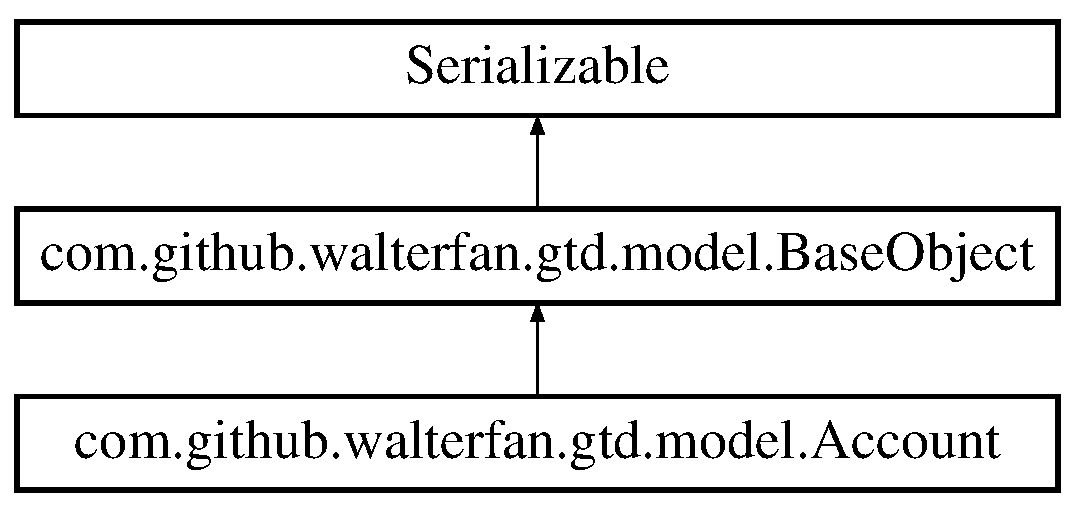
\includegraphics[height=3.000000cm]{classcom_1_1github_1_1walterfan_1_1gtd_1_1model_1_1Account}
\end{center}
\end{figure}
\subsection*{Public Member Functions}
\begin{DoxyCompactItemize}
\item 
String \hyperlink{classcom_1_1github_1_1walterfan_1_1gtd_1_1model_1_1Account_acebe7fcd66c00569d05b522aff45df1d}{get\-User\-Name} ()
\item 
void \hyperlink{classcom_1_1github_1_1walterfan_1_1gtd_1_1model_1_1Account_a439d336f89b4fa9d300f839c0c84cd4b}{set\-User\-Name} (String user\-Name)
\item 
String \hyperlink{classcom_1_1github_1_1walterfan_1_1gtd_1_1model_1_1Account_a30b5e49f894fac9c2d8768e1d6af9754}{get\-Password} ()
\item 
void \hyperlink{classcom_1_1github_1_1walterfan_1_1gtd_1_1model_1_1Account_ac4f3dcd5830b8ea46d3baf850be762ab}{set\-Password} (String password)
\item 
String \hyperlink{classcom_1_1github_1_1walterfan_1_1gtd_1_1model_1_1Account_af4348da0ca9d60c7ac22c98909a48b6e}{get\-Email} ()
\item 
void \hyperlink{classcom_1_1github_1_1walterfan_1_1gtd_1_1model_1_1Account_ad8b537f30d7aef17335055d6fdb638b7}{set\-Email} (String email)
\item 
\hypertarget{classcom_1_1github_1_1walterfan_1_1gtd_1_1model_1_1Account_a924d8d80500d6a18c7bc3132ce65872b}{String {\bfseries to\-Xml} ()}\label{classcom_1_1github_1_1walterfan_1_1gtd_1_1model_1_1Account_a924d8d80500d6a18c7bc3132ce65872b}

\item 
\hypertarget{classcom_1_1github_1_1walterfan_1_1gtd_1_1model_1_1Account_a568a57aef35d6860c2a5066c4b7a8240}{String {\bfseries get\-Site\-Name} ()}\label{classcom_1_1github_1_1walterfan_1_1gtd_1_1model_1_1Account_a568a57aef35d6860c2a5066c4b7a8240}

\item 
\hypertarget{classcom_1_1github_1_1walterfan_1_1gtd_1_1model_1_1Account_ac414b3eaac18d17a03c8c421b4187fb8}{void {\bfseries set\-Site\-Name} (String site\-Name)}\label{classcom_1_1github_1_1walterfan_1_1gtd_1_1model_1_1Account_ac414b3eaac18d17a03c8c421b4187fb8}

\item 
\hypertarget{classcom_1_1github_1_1walterfan_1_1gtd_1_1model_1_1Account_a6628cc4464884740c70f0b9e1428d05e}{String {\bfseries get\-Site\-Url} ()}\label{classcom_1_1github_1_1walterfan_1_1gtd_1_1model_1_1Account_a6628cc4464884740c70f0b9e1428d05e}

\item 
\hypertarget{classcom_1_1github_1_1walterfan_1_1gtd_1_1model_1_1Account_a426e0c7236513ed7336b0e7113b75f25}{void {\bfseries set\-Site\-Url} (String site\-Url)}\label{classcom_1_1github_1_1walterfan_1_1gtd_1_1model_1_1Account_a426e0c7236513ed7336b0e7113b75f25}

\item 
int \hyperlink{classcom_1_1github_1_1walterfan_1_1gtd_1_1model_1_1Account_a56496c02e5d9de99edcee842ab9b1cde}{get\-User\-I\-D} ()
\item 
void \hyperlink{classcom_1_1github_1_1walterfan_1_1gtd_1_1model_1_1Account_a71f986061d9fdb6209e14c24492fd22a}{set\-User\-I\-D} (int user\-I\-D)
\item 
int \hyperlink{classcom_1_1github_1_1walterfan_1_1gtd_1_1model_1_1Account_ab52eebb5e3ec4be02a9f826c8b21267a}{get\-Account\-I\-D} ()
\item 
void \hyperlink{classcom_1_1github_1_1walterfan_1_1gtd_1_1model_1_1Account_a5b660abc2c5399dacf0d750e655676cb}{set\-Account\-I\-D} (int account\-I\-D)
\end{DoxyCompactItemize}
\subsection*{Additional Inherited Members}


\subsection{Detailed Description}


Definition at line 7 of file Account.\-java.



\subsection{Member Function Documentation}
\hypertarget{classcom_1_1github_1_1walterfan_1_1gtd_1_1model_1_1Account_ab52eebb5e3ec4be02a9f826c8b21267a}{\index{com\-::github\-::walterfan\-::gtd\-::model\-::\-Account@{com\-::github\-::walterfan\-::gtd\-::model\-::\-Account}!get\-Account\-I\-D@{get\-Account\-I\-D}}
\index{get\-Account\-I\-D@{get\-Account\-I\-D}!com::github::walterfan::gtd::model::Account@{com\-::github\-::walterfan\-::gtd\-::model\-::\-Account}}
\subsubsection[{get\-Account\-I\-D}]{\setlength{\rightskip}{0pt plus 5cm}int com.\-github.\-walterfan.\-gtd.\-model.\-Account.\-get\-Account\-I\-D (
\begin{DoxyParamCaption}
{}
\end{DoxyParamCaption}
)\hspace{0.3cm}{\ttfamily [inline]}}}\label{classcom_1_1github_1_1walterfan_1_1gtd_1_1model_1_1Account_ab52eebb5e3ec4be02a9f826c8b21267a}
\begin{DoxyReturn}{Returns}
the account\-I\-D 
\end{DoxyReturn}


Definition at line 114 of file Account.\-java.


\begin{DoxyCode}
114                               \{
115         \textcolor{keywordflow}{return} accountID;
116     \}
\end{DoxyCode}
\hypertarget{classcom_1_1github_1_1walterfan_1_1gtd_1_1model_1_1Account_af4348da0ca9d60c7ac22c98909a48b6e}{\index{com\-::github\-::walterfan\-::gtd\-::model\-::\-Account@{com\-::github\-::walterfan\-::gtd\-::model\-::\-Account}!get\-Email@{get\-Email}}
\index{get\-Email@{get\-Email}!com::github::walterfan::gtd::model::Account@{com\-::github\-::walterfan\-::gtd\-::model\-::\-Account}}
\subsubsection[{get\-Email}]{\setlength{\rightskip}{0pt plus 5cm}String com.\-github.\-walterfan.\-gtd.\-model.\-Account.\-get\-Email (
\begin{DoxyParamCaption}
{}
\end{DoxyParamCaption}
)\hspace{0.3cm}{\ttfamily [inline]}}}\label{classcom_1_1github_1_1walterfan_1_1gtd_1_1model_1_1Account_af4348da0ca9d60c7ac22c98909a48b6e}
\begin{DoxyReturn}{Returns}
the email 
\end{DoxyReturn}


Definition at line 52 of file Account.\-java.


\begin{DoxyCode}
52                              \{
53         \textcolor{keywordflow}{return} email;
54     \}
\end{DoxyCode}
\hypertarget{classcom_1_1github_1_1walterfan_1_1gtd_1_1model_1_1Account_a30b5e49f894fac9c2d8768e1d6af9754}{\index{com\-::github\-::walterfan\-::gtd\-::model\-::\-Account@{com\-::github\-::walterfan\-::gtd\-::model\-::\-Account}!get\-Password@{get\-Password}}
\index{get\-Password@{get\-Password}!com::github::walterfan::gtd::model::Account@{com\-::github\-::walterfan\-::gtd\-::model\-::\-Account}}
\subsubsection[{get\-Password}]{\setlength{\rightskip}{0pt plus 5cm}String com.\-github.\-walterfan.\-gtd.\-model.\-Account.\-get\-Password (
\begin{DoxyParamCaption}
{}
\end{DoxyParamCaption}
)\hspace{0.3cm}{\ttfamily [inline]}}}\label{classcom_1_1github_1_1walterfan_1_1gtd_1_1model_1_1Account_a30b5e49f894fac9c2d8768e1d6af9754}
\begin{DoxyReturn}{Returns}
the password 
\end{DoxyReturn}


Definition at line 36 of file Account.\-java.


\begin{DoxyCode}
36                                 \{
37         \textcolor{keywordflow}{return} password;
38     \}
\end{DoxyCode}
\hypertarget{classcom_1_1github_1_1walterfan_1_1gtd_1_1model_1_1Account_a56496c02e5d9de99edcee842ab9b1cde}{\index{com\-::github\-::walterfan\-::gtd\-::model\-::\-Account@{com\-::github\-::walterfan\-::gtd\-::model\-::\-Account}!get\-User\-I\-D@{get\-User\-I\-D}}
\index{get\-User\-I\-D@{get\-User\-I\-D}!com::github::walterfan::gtd::model::Account@{com\-::github\-::walterfan\-::gtd\-::model\-::\-Account}}
\subsubsection[{get\-User\-I\-D}]{\setlength{\rightskip}{0pt plus 5cm}int com.\-github.\-walterfan.\-gtd.\-model.\-Account.\-get\-User\-I\-D (
\begin{DoxyParamCaption}
{}
\end{DoxyParamCaption}
)\hspace{0.3cm}{\ttfamily [inline]}}}\label{classcom_1_1github_1_1walterfan_1_1gtd_1_1model_1_1Account_a56496c02e5d9de99edcee842ab9b1cde}
\begin{DoxyReturn}{Returns}
the user\-I\-D 
\end{DoxyReturn}


Definition at line 98 of file Account.\-java.


\begin{DoxyCode}
98                            \{
99         \textcolor{keywordflow}{return} userID;
100     \}
\end{DoxyCode}
\hypertarget{classcom_1_1github_1_1walterfan_1_1gtd_1_1model_1_1Account_acebe7fcd66c00569d05b522aff45df1d}{\index{com\-::github\-::walterfan\-::gtd\-::model\-::\-Account@{com\-::github\-::walterfan\-::gtd\-::model\-::\-Account}!get\-User\-Name@{get\-User\-Name}}
\index{get\-User\-Name@{get\-User\-Name}!com::github::walterfan::gtd::model::Account@{com\-::github\-::walterfan\-::gtd\-::model\-::\-Account}}
\subsubsection[{get\-User\-Name}]{\setlength{\rightskip}{0pt plus 5cm}String com.\-github.\-walterfan.\-gtd.\-model.\-Account.\-get\-User\-Name (
\begin{DoxyParamCaption}
{}
\end{DoxyParamCaption}
)\hspace{0.3cm}{\ttfamily [inline]}}}\label{classcom_1_1github_1_1walterfan_1_1gtd_1_1model_1_1Account_acebe7fcd66c00569d05b522aff45df1d}
\begin{DoxyReturn}{Returns}
the user\-Name 
\end{DoxyReturn}


Definition at line 22 of file Account.\-java.


\begin{DoxyCode}
22                                 \{
23         \textcolor{keywordflow}{return} userName;
24     \}
\end{DoxyCode}
\hypertarget{classcom_1_1github_1_1walterfan_1_1gtd_1_1model_1_1Account_a5b660abc2c5399dacf0d750e655676cb}{\index{com\-::github\-::walterfan\-::gtd\-::model\-::\-Account@{com\-::github\-::walterfan\-::gtd\-::model\-::\-Account}!set\-Account\-I\-D@{set\-Account\-I\-D}}
\index{set\-Account\-I\-D@{set\-Account\-I\-D}!com::github::walterfan::gtd::model::Account@{com\-::github\-::walterfan\-::gtd\-::model\-::\-Account}}
\subsubsection[{set\-Account\-I\-D}]{\setlength{\rightskip}{0pt plus 5cm}void com.\-github.\-walterfan.\-gtd.\-model.\-Account.\-set\-Account\-I\-D (
\begin{DoxyParamCaption}
\item[{int}]{account\-I\-D}
\end{DoxyParamCaption}
)\hspace{0.3cm}{\ttfamily [inline]}}}\label{classcom_1_1github_1_1walterfan_1_1gtd_1_1model_1_1Account_a5b660abc2c5399dacf0d750e655676cb}

\begin{DoxyParams}{Parameters}
{\em account\-I\-D} & the account\-I\-D to set \\
\hline
\end{DoxyParams}


Definition at line 122 of file Account.\-java.


\begin{DoxyCode}
122                                             \{
123         this.accountID = accountID;
124     \}
\end{DoxyCode}
\hypertarget{classcom_1_1github_1_1walterfan_1_1gtd_1_1model_1_1Account_ad8b537f30d7aef17335055d6fdb638b7}{\index{com\-::github\-::walterfan\-::gtd\-::model\-::\-Account@{com\-::github\-::walterfan\-::gtd\-::model\-::\-Account}!set\-Email@{set\-Email}}
\index{set\-Email@{set\-Email}!com::github::walterfan::gtd::model::Account@{com\-::github\-::walterfan\-::gtd\-::model\-::\-Account}}
\subsubsection[{set\-Email}]{\setlength{\rightskip}{0pt plus 5cm}void com.\-github.\-walterfan.\-gtd.\-model.\-Account.\-set\-Email (
\begin{DoxyParamCaption}
\item[{String}]{email}
\end{DoxyParamCaption}
)\hspace{0.3cm}{\ttfamily [inline]}}}\label{classcom_1_1github_1_1walterfan_1_1gtd_1_1model_1_1Account_ad8b537f30d7aef17335055d6fdb638b7}

\begin{DoxyParams}{Parameters}
{\em email} & the email to set \\
\hline
\end{DoxyParams}


Definition at line 59 of file Account.\-java.


\begin{DoxyCode}
59                                        \{
60         this.email = email;
61     \}
\end{DoxyCode}
\hypertarget{classcom_1_1github_1_1walterfan_1_1gtd_1_1model_1_1Account_ac4f3dcd5830b8ea46d3baf850be762ab}{\index{com\-::github\-::walterfan\-::gtd\-::model\-::\-Account@{com\-::github\-::walterfan\-::gtd\-::model\-::\-Account}!set\-Password@{set\-Password}}
\index{set\-Password@{set\-Password}!com::github::walterfan::gtd::model::Account@{com\-::github\-::walterfan\-::gtd\-::model\-::\-Account}}
\subsubsection[{set\-Password}]{\setlength{\rightskip}{0pt plus 5cm}void com.\-github.\-walterfan.\-gtd.\-model.\-Account.\-set\-Password (
\begin{DoxyParamCaption}
\item[{String}]{password}
\end{DoxyParamCaption}
)\hspace{0.3cm}{\ttfamily [inline]}}}\label{classcom_1_1github_1_1walterfan_1_1gtd_1_1model_1_1Account_ac4f3dcd5830b8ea46d3baf850be762ab}

\begin{DoxyParams}{Parameters}
{\em password} & the password to set \\
\hline
\end{DoxyParams}


Definition at line 43 of file Account.\-java.


\begin{DoxyCode}
43                                              \{
44         this.password = password;
45     \}
\end{DoxyCode}
\hypertarget{classcom_1_1github_1_1walterfan_1_1gtd_1_1model_1_1Account_a71f986061d9fdb6209e14c24492fd22a}{\index{com\-::github\-::walterfan\-::gtd\-::model\-::\-Account@{com\-::github\-::walterfan\-::gtd\-::model\-::\-Account}!set\-User\-I\-D@{set\-User\-I\-D}}
\index{set\-User\-I\-D@{set\-User\-I\-D}!com::github::walterfan::gtd::model::Account@{com\-::github\-::walterfan\-::gtd\-::model\-::\-Account}}
\subsubsection[{set\-User\-I\-D}]{\setlength{\rightskip}{0pt plus 5cm}void com.\-github.\-walterfan.\-gtd.\-model.\-Account.\-set\-User\-I\-D (
\begin{DoxyParamCaption}
\item[{int}]{user\-I\-D}
\end{DoxyParamCaption}
)\hspace{0.3cm}{\ttfamily [inline]}}}\label{classcom_1_1github_1_1walterfan_1_1gtd_1_1model_1_1Account_a71f986061d9fdb6209e14c24492fd22a}

\begin{DoxyParams}{Parameters}
{\em user\-I\-D} & the user\-I\-D to set \\
\hline
\end{DoxyParams}


Definition at line 106 of file Account.\-java.


\begin{DoxyCode}
106                                       \{
107         this.userID = userID;
108     \}
\end{DoxyCode}
\hypertarget{classcom_1_1github_1_1walterfan_1_1gtd_1_1model_1_1Account_a439d336f89b4fa9d300f839c0c84cd4b}{\index{com\-::github\-::walterfan\-::gtd\-::model\-::\-Account@{com\-::github\-::walterfan\-::gtd\-::model\-::\-Account}!set\-User\-Name@{set\-User\-Name}}
\index{set\-User\-Name@{set\-User\-Name}!com::github::walterfan::gtd::model::Account@{com\-::github\-::walterfan\-::gtd\-::model\-::\-Account}}
\subsubsection[{set\-User\-Name}]{\setlength{\rightskip}{0pt plus 5cm}void com.\-github.\-walterfan.\-gtd.\-model.\-Account.\-set\-User\-Name (
\begin{DoxyParamCaption}
\item[{String}]{user\-Name}
\end{DoxyParamCaption}
)\hspace{0.3cm}{\ttfamily [inline]}}}\label{classcom_1_1github_1_1walterfan_1_1gtd_1_1model_1_1Account_a439d336f89b4fa9d300f839c0c84cd4b}

\begin{DoxyParams}{Parameters}
{\em user\-Name} & the user\-Name to set \\
\hline
\end{DoxyParams}


Definition at line 29 of file Account.\-java.


\begin{DoxyCode}
29                                              \{
30         this.userName = userName;
31     \}
\end{DoxyCode}


The documentation for this class was generated from the following file\-:\begin{DoxyCompactItemize}
\item 
/cygdrive/d/workspace/java/\-G\-T\-D/src/com/github/walterfan/gtd/model/Account.\-java\end{DoxyCompactItemize}

\hypertarget{classcom_1_1github_1_1walterfan_1_1gtd_1_1model_1_1Article}{\section{com.\-github.\-walterfan.\-gtd.\-model.\-Article Class Reference}
\label{classcom_1_1github_1_1walterfan_1_1gtd_1_1model_1_1Article}\index{com.\-github.\-walterfan.\-gtd.\-model.\-Article@{com.\-github.\-walterfan.\-gtd.\-model.\-Article}}
}
Inheritance diagram for com.\-github.\-walterfan.\-gtd.\-model.\-Article\-:\begin{figure}[H]
\begin{center}
\leavevmode
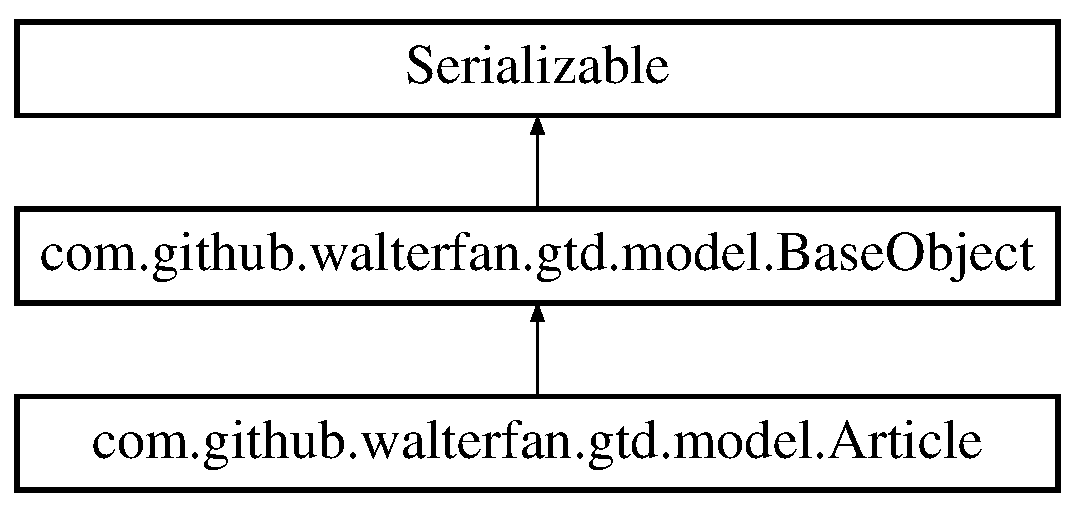
\includegraphics[height=3.000000cm]{classcom_1_1github_1_1walterfan_1_1gtd_1_1model_1_1Article}
\end{center}
\end{figure}
\subsection*{Public Member Functions}
\begin{DoxyCompactItemize}
\item 
String \hyperlink{classcom_1_1github_1_1walterfan_1_1gtd_1_1model_1_1Article_a4650ebf856f53b5197324a67e1684b41}{get\-Keywords} ()
\item 
void \hyperlink{classcom_1_1github_1_1walterfan_1_1gtd_1_1model_1_1Article_a37a35e568e1211352ab4aee01efc2850}{set\-Keywords} (String keywords)
\item 
String \hyperlink{classcom_1_1github_1_1walterfan_1_1gtd_1_1model_1_1Article_a3a75e72a454b1027a456f7d09adf7841}{get\-Topic} ()
\item 
void \hyperlink{classcom_1_1github_1_1walterfan_1_1gtd_1_1model_1_1Article_af54797f3f70167cf81199d6ddb3abd6d}{set\-Topic} (String topic)
\item 
String \hyperlink{classcom_1_1github_1_1walterfan_1_1gtd_1_1model_1_1Article_a817c646f979cf5e6459f24bbdc815569}{get\-Content} ()
\item 
void \hyperlink{classcom_1_1github_1_1walterfan_1_1gtd_1_1model_1_1Article_a2dc8128e159ea5202a9a6cfa7c92ac9c}{set\-Content} (String content)
\item 
int \hyperlink{classcom_1_1github_1_1walterfan_1_1gtd_1_1model_1_1Article_a72a6a6682a8a6c101b0d3ebc822a7c8d}{get\-User\-I\-D} ()
\item 
void \hyperlink{classcom_1_1github_1_1walterfan_1_1gtd_1_1model_1_1Article_a2258f8798d107e9fb7bb8eb20542c9af}{set\-User\-I\-D} (int user\-I\-D)
\item 
int \hyperlink{classcom_1_1github_1_1walterfan_1_1gtd_1_1model_1_1Article_ae2fdd0a0677ec8c432074a35dec2bae7}{get\-Category\-I\-D} ()
\item 
void \hyperlink{classcom_1_1github_1_1walterfan_1_1gtd_1_1model_1_1Article_ac3439300f13e7541de8ccc5a326ad6e0}{set\-Category\-I\-D} (int category\-I\-D)
\item 
int \hyperlink{classcom_1_1github_1_1walterfan_1_1gtd_1_1model_1_1Article_ab897bba6f41a799cae31f5208910c526}{get\-Article\-I\-D} ()
\item 
void \hyperlink{classcom_1_1github_1_1walterfan_1_1gtd_1_1model_1_1Article_a2b08cb4a33bf65e3751e1f20fc1816bf}{set\-Article\-I\-D} (int article\-I\-D)
\item 
Date \hyperlink{classcom_1_1github_1_1walterfan_1_1gtd_1_1model_1_1Article_a7dc311a5adcb38f8e1bfce3e8d012671}{get\-Create\-Time} ()
\item 
void \hyperlink{classcom_1_1github_1_1walterfan_1_1gtd_1_1model_1_1Article_aa27ee0b3fb32c1e00942b7c7da479b74}{set\-Create\-Time} (Date create\-Time)
\end{DoxyCompactItemize}
\subsection*{Additional Inherited Members}


\subsection{Detailed Description}


Definition at line 6 of file Article.\-java.



\subsection{Member Function Documentation}
\hypertarget{classcom_1_1github_1_1walterfan_1_1gtd_1_1model_1_1Article_ab897bba6f41a799cae31f5208910c526}{\index{com\-::github\-::walterfan\-::gtd\-::model\-::\-Article@{com\-::github\-::walterfan\-::gtd\-::model\-::\-Article}!get\-Article\-I\-D@{get\-Article\-I\-D}}
\index{get\-Article\-I\-D@{get\-Article\-I\-D}!com::github::walterfan::gtd::model::Article@{com\-::github\-::walterfan\-::gtd\-::model\-::\-Article}}
\subsubsection[{get\-Article\-I\-D}]{\setlength{\rightskip}{0pt plus 5cm}int com.\-github.\-walterfan.\-gtd.\-model.\-Article.\-get\-Article\-I\-D (
\begin{DoxyParamCaption}
{}
\end{DoxyParamCaption}
)\hspace{0.3cm}{\ttfamily [inline]}}}\label{classcom_1_1github_1_1walterfan_1_1gtd_1_1model_1_1Article_ab897bba6f41a799cae31f5208910c526}
\begin{DoxyReturn}{Returns}
the article\-I\-D 
\end{DoxyReturn}


Definition at line 98 of file Article.\-java.


\begin{DoxyCode}
98                               \{
99         \textcolor{keywordflow}{return} articleID;
100     \}
\end{DoxyCode}
\hypertarget{classcom_1_1github_1_1walterfan_1_1gtd_1_1model_1_1Article_ae2fdd0a0677ec8c432074a35dec2bae7}{\index{com\-::github\-::walterfan\-::gtd\-::model\-::\-Article@{com\-::github\-::walterfan\-::gtd\-::model\-::\-Article}!get\-Category\-I\-D@{get\-Category\-I\-D}}
\index{get\-Category\-I\-D@{get\-Category\-I\-D}!com::github::walterfan::gtd::model::Article@{com\-::github\-::walterfan\-::gtd\-::model\-::\-Article}}
\subsubsection[{get\-Category\-I\-D}]{\setlength{\rightskip}{0pt plus 5cm}int com.\-github.\-walterfan.\-gtd.\-model.\-Article.\-get\-Category\-I\-D (
\begin{DoxyParamCaption}
{}
\end{DoxyParamCaption}
)\hspace{0.3cm}{\ttfamily [inline]}}}\label{classcom_1_1github_1_1walterfan_1_1gtd_1_1model_1_1Article_ae2fdd0a0677ec8c432074a35dec2bae7}
\begin{DoxyReturn}{Returns}
the category\-I\-D 
\end{DoxyReturn}


Definition at line 82 of file Article.\-java.


\begin{DoxyCode}
82                                \{
83         \textcolor{keywordflow}{return} categoryID;
84     \}
\end{DoxyCode}
\hypertarget{classcom_1_1github_1_1walterfan_1_1gtd_1_1model_1_1Article_a817c646f979cf5e6459f24bbdc815569}{\index{com\-::github\-::walterfan\-::gtd\-::model\-::\-Article@{com\-::github\-::walterfan\-::gtd\-::model\-::\-Article}!get\-Content@{get\-Content}}
\index{get\-Content@{get\-Content}!com::github::walterfan::gtd::model::Article@{com\-::github\-::walterfan\-::gtd\-::model\-::\-Article}}
\subsubsection[{get\-Content}]{\setlength{\rightskip}{0pt plus 5cm}String com.\-github.\-walterfan.\-gtd.\-model.\-Article.\-get\-Content (
\begin{DoxyParamCaption}
{}
\end{DoxyParamCaption}
)\hspace{0.3cm}{\ttfamily [inline]}}}\label{classcom_1_1github_1_1walterfan_1_1gtd_1_1model_1_1Article_a817c646f979cf5e6459f24bbdc815569}
\begin{DoxyReturn}{Returns}
the content 
\end{DoxyReturn}


Definition at line 49 of file Article.\-java.


\begin{DoxyCode}
49                                \{
50         \textcolor{keywordflow}{return} content;
51     \}
\end{DoxyCode}
\hypertarget{classcom_1_1github_1_1walterfan_1_1gtd_1_1model_1_1Article_a7dc311a5adcb38f8e1bfce3e8d012671}{\index{com\-::github\-::walterfan\-::gtd\-::model\-::\-Article@{com\-::github\-::walterfan\-::gtd\-::model\-::\-Article}!get\-Create\-Time@{get\-Create\-Time}}
\index{get\-Create\-Time@{get\-Create\-Time}!com::github::walterfan::gtd::model::Article@{com\-::github\-::walterfan\-::gtd\-::model\-::\-Article}}
\subsubsection[{get\-Create\-Time}]{\setlength{\rightskip}{0pt plus 5cm}Date com.\-github.\-walterfan.\-gtd.\-model.\-Article.\-get\-Create\-Time (
\begin{DoxyParamCaption}
{}
\end{DoxyParamCaption}
)\hspace{0.3cm}{\ttfamily [inline]}}}\label{classcom_1_1github_1_1walterfan_1_1gtd_1_1model_1_1Article_a7dc311a5adcb38f8e1bfce3e8d012671}
\begin{DoxyReturn}{Returns}
the create\-Time 
\end{DoxyReturn}


Definition at line 114 of file Article.\-java.


\begin{DoxyCode}
114                                 \{
115         \textcolor{keywordflow}{return} createTime;
116     \}
\end{DoxyCode}
\hypertarget{classcom_1_1github_1_1walterfan_1_1gtd_1_1model_1_1Article_a4650ebf856f53b5197324a67e1684b41}{\index{com\-::github\-::walterfan\-::gtd\-::model\-::\-Article@{com\-::github\-::walterfan\-::gtd\-::model\-::\-Article}!get\-Keywords@{get\-Keywords}}
\index{get\-Keywords@{get\-Keywords}!com::github::walterfan::gtd::model::Article@{com\-::github\-::walterfan\-::gtd\-::model\-::\-Article}}
\subsubsection[{get\-Keywords}]{\setlength{\rightskip}{0pt plus 5cm}String com.\-github.\-walterfan.\-gtd.\-model.\-Article.\-get\-Keywords (
\begin{DoxyParamCaption}
{}
\end{DoxyParamCaption}
)\hspace{0.3cm}{\ttfamily [inline]}}}\label{classcom_1_1github_1_1walterfan_1_1gtd_1_1model_1_1Article_a4650ebf856f53b5197324a67e1684b41}
\begin{DoxyReturn}{Returns}
the keywords 
\end{DoxyReturn}


Definition at line 18 of file Article.\-java.


\begin{DoxyCode}
18                                 \{
19         \textcolor{keywordflow}{return} keywords;
20     \}
\end{DoxyCode}
\hypertarget{classcom_1_1github_1_1walterfan_1_1gtd_1_1model_1_1Article_a3a75e72a454b1027a456f7d09adf7841}{\index{com\-::github\-::walterfan\-::gtd\-::model\-::\-Article@{com\-::github\-::walterfan\-::gtd\-::model\-::\-Article}!get\-Topic@{get\-Topic}}
\index{get\-Topic@{get\-Topic}!com::github::walterfan::gtd::model::Article@{com\-::github\-::walterfan\-::gtd\-::model\-::\-Article}}
\subsubsection[{get\-Topic}]{\setlength{\rightskip}{0pt plus 5cm}String com.\-github.\-walterfan.\-gtd.\-model.\-Article.\-get\-Topic (
\begin{DoxyParamCaption}
{}
\end{DoxyParamCaption}
)\hspace{0.3cm}{\ttfamily [inline]}}}\label{classcom_1_1github_1_1walterfan_1_1gtd_1_1model_1_1Article_a3a75e72a454b1027a456f7d09adf7841}
\begin{DoxyReturn}{Returns}
the topic 
\end{DoxyReturn}


Definition at line 33 of file Article.\-java.


\begin{DoxyCode}
33                              \{
34         \textcolor{keywordflow}{return} topic;
35     \}
\end{DoxyCode}
\hypertarget{classcom_1_1github_1_1walterfan_1_1gtd_1_1model_1_1Article_a72a6a6682a8a6c101b0d3ebc822a7c8d}{\index{com\-::github\-::walterfan\-::gtd\-::model\-::\-Article@{com\-::github\-::walterfan\-::gtd\-::model\-::\-Article}!get\-User\-I\-D@{get\-User\-I\-D}}
\index{get\-User\-I\-D@{get\-User\-I\-D}!com::github::walterfan::gtd::model::Article@{com\-::github\-::walterfan\-::gtd\-::model\-::\-Article}}
\subsubsection[{get\-User\-I\-D}]{\setlength{\rightskip}{0pt plus 5cm}int com.\-github.\-walterfan.\-gtd.\-model.\-Article.\-get\-User\-I\-D (
\begin{DoxyParamCaption}
{}
\end{DoxyParamCaption}
)\hspace{0.3cm}{\ttfamily [inline]}}}\label{classcom_1_1github_1_1walterfan_1_1gtd_1_1model_1_1Article_a72a6a6682a8a6c101b0d3ebc822a7c8d}
\begin{DoxyReturn}{Returns}
the user\-I\-D 
\end{DoxyReturn}


Definition at line 66 of file Article.\-java.


\begin{DoxyCode}
66                            \{
67         \textcolor{keywordflow}{return} userID;
68     \}
\end{DoxyCode}
\hypertarget{classcom_1_1github_1_1walterfan_1_1gtd_1_1model_1_1Article_a2b08cb4a33bf65e3751e1f20fc1816bf}{\index{com\-::github\-::walterfan\-::gtd\-::model\-::\-Article@{com\-::github\-::walterfan\-::gtd\-::model\-::\-Article}!set\-Article\-I\-D@{set\-Article\-I\-D}}
\index{set\-Article\-I\-D@{set\-Article\-I\-D}!com::github::walterfan::gtd::model::Article@{com\-::github\-::walterfan\-::gtd\-::model\-::\-Article}}
\subsubsection[{set\-Article\-I\-D}]{\setlength{\rightskip}{0pt plus 5cm}void com.\-github.\-walterfan.\-gtd.\-model.\-Article.\-set\-Article\-I\-D (
\begin{DoxyParamCaption}
\item[{int}]{article\-I\-D}
\end{DoxyParamCaption}
)\hspace{0.3cm}{\ttfamily [inline]}}}\label{classcom_1_1github_1_1walterfan_1_1gtd_1_1model_1_1Article_a2b08cb4a33bf65e3751e1f20fc1816bf}

\begin{DoxyParams}{Parameters}
{\em article\-I\-D} & the article\-I\-D to set \\
\hline
\end{DoxyParams}


Definition at line 106 of file Article.\-java.


\begin{DoxyCode}
106                                             \{
107         this.articleID = articleID;
108     \}
\end{DoxyCode}
\hypertarget{classcom_1_1github_1_1walterfan_1_1gtd_1_1model_1_1Article_ac3439300f13e7541de8ccc5a326ad6e0}{\index{com\-::github\-::walterfan\-::gtd\-::model\-::\-Article@{com\-::github\-::walterfan\-::gtd\-::model\-::\-Article}!set\-Category\-I\-D@{set\-Category\-I\-D}}
\index{set\-Category\-I\-D@{set\-Category\-I\-D}!com::github::walterfan::gtd::model::Article@{com\-::github\-::walterfan\-::gtd\-::model\-::\-Article}}
\subsubsection[{set\-Category\-I\-D}]{\setlength{\rightskip}{0pt plus 5cm}void com.\-github.\-walterfan.\-gtd.\-model.\-Article.\-set\-Category\-I\-D (
\begin{DoxyParamCaption}
\item[{int}]{category\-I\-D}
\end{DoxyParamCaption}
)\hspace{0.3cm}{\ttfamily [inline]}}}\label{classcom_1_1github_1_1walterfan_1_1gtd_1_1model_1_1Article_ac3439300f13e7541de8ccc5a326ad6e0}

\begin{DoxyParams}{Parameters}
{\em category\-I\-D} & the category\-I\-D to set \\
\hline
\end{DoxyParams}


Definition at line 90 of file Article.\-java.


\begin{DoxyCode}
90                                               \{
91         this.categoryID = categoryID;
92     \}
\end{DoxyCode}
\hypertarget{classcom_1_1github_1_1walterfan_1_1gtd_1_1model_1_1Article_a2dc8128e159ea5202a9a6cfa7c92ac9c}{\index{com\-::github\-::walterfan\-::gtd\-::model\-::\-Article@{com\-::github\-::walterfan\-::gtd\-::model\-::\-Article}!set\-Content@{set\-Content}}
\index{set\-Content@{set\-Content}!com::github::walterfan::gtd::model::Article@{com\-::github\-::walterfan\-::gtd\-::model\-::\-Article}}
\subsubsection[{set\-Content}]{\setlength{\rightskip}{0pt plus 5cm}void com.\-github.\-walterfan.\-gtd.\-model.\-Article.\-set\-Content (
\begin{DoxyParamCaption}
\item[{String}]{content}
\end{DoxyParamCaption}
)\hspace{0.3cm}{\ttfamily [inline]}}}\label{classcom_1_1github_1_1walterfan_1_1gtd_1_1model_1_1Article_a2dc8128e159ea5202a9a6cfa7c92ac9c}

\begin{DoxyParams}{Parameters}
{\em content} & the content to set \\
\hline
\end{DoxyParams}


Definition at line 57 of file Article.\-java.


\begin{DoxyCode}
57                                            \{
58         this.content = content;
59     \}
\end{DoxyCode}
\hypertarget{classcom_1_1github_1_1walterfan_1_1gtd_1_1model_1_1Article_aa27ee0b3fb32c1e00942b7c7da479b74}{\index{com\-::github\-::walterfan\-::gtd\-::model\-::\-Article@{com\-::github\-::walterfan\-::gtd\-::model\-::\-Article}!set\-Create\-Time@{set\-Create\-Time}}
\index{set\-Create\-Time@{set\-Create\-Time}!com::github::walterfan::gtd::model::Article@{com\-::github\-::walterfan\-::gtd\-::model\-::\-Article}}
\subsubsection[{set\-Create\-Time}]{\setlength{\rightskip}{0pt plus 5cm}void com.\-github.\-walterfan.\-gtd.\-model.\-Article.\-set\-Create\-Time (
\begin{DoxyParamCaption}
\item[{Date}]{create\-Time}
\end{DoxyParamCaption}
)\hspace{0.3cm}{\ttfamily [inline]}}}\label{classcom_1_1github_1_1walterfan_1_1gtd_1_1model_1_1Article_aa27ee0b3fb32c1e00942b7c7da479b74}

\begin{DoxyParams}{Parameters}
{\em create\-Time} & the create\-Time to set \\
\hline
\end{DoxyParams}


Definition at line 122 of file Article.\-java.


\begin{DoxyCode}
122                                                \{
123         this.createTime = createTime;
124     \}
\end{DoxyCode}
\hypertarget{classcom_1_1github_1_1walterfan_1_1gtd_1_1model_1_1Article_a37a35e568e1211352ab4aee01efc2850}{\index{com\-::github\-::walterfan\-::gtd\-::model\-::\-Article@{com\-::github\-::walterfan\-::gtd\-::model\-::\-Article}!set\-Keywords@{set\-Keywords}}
\index{set\-Keywords@{set\-Keywords}!com::github::walterfan::gtd::model::Article@{com\-::github\-::walterfan\-::gtd\-::model\-::\-Article}}
\subsubsection[{set\-Keywords}]{\setlength{\rightskip}{0pt plus 5cm}void com.\-github.\-walterfan.\-gtd.\-model.\-Article.\-set\-Keywords (
\begin{DoxyParamCaption}
\item[{String}]{keywords}
\end{DoxyParamCaption}
)\hspace{0.3cm}{\ttfamily [inline]}}}\label{classcom_1_1github_1_1walterfan_1_1gtd_1_1model_1_1Article_a37a35e568e1211352ab4aee01efc2850}

\begin{DoxyParams}{Parameters}
{\em keywords} & the keywords to set \\
\hline
\end{DoxyParams}


Definition at line 25 of file Article.\-java.


\begin{DoxyCode}
25                                              \{
26         this.keywords = keywords;
27     \}
\end{DoxyCode}
\hypertarget{classcom_1_1github_1_1walterfan_1_1gtd_1_1model_1_1Article_af54797f3f70167cf81199d6ddb3abd6d}{\index{com\-::github\-::walterfan\-::gtd\-::model\-::\-Article@{com\-::github\-::walterfan\-::gtd\-::model\-::\-Article}!set\-Topic@{set\-Topic}}
\index{set\-Topic@{set\-Topic}!com::github::walterfan::gtd::model::Article@{com\-::github\-::walterfan\-::gtd\-::model\-::\-Article}}
\subsubsection[{set\-Topic}]{\setlength{\rightskip}{0pt plus 5cm}void com.\-github.\-walterfan.\-gtd.\-model.\-Article.\-set\-Topic (
\begin{DoxyParamCaption}
\item[{String}]{topic}
\end{DoxyParamCaption}
)\hspace{0.3cm}{\ttfamily [inline]}}}\label{classcom_1_1github_1_1walterfan_1_1gtd_1_1model_1_1Article_af54797f3f70167cf81199d6ddb3abd6d}

\begin{DoxyParams}{Parameters}
{\em topic} & the topic to set \\
\hline
\end{DoxyParams}


Definition at line 41 of file Article.\-java.


\begin{DoxyCode}
41                                        \{
42         this.topic = topic;
43     \}
\end{DoxyCode}
\hypertarget{classcom_1_1github_1_1walterfan_1_1gtd_1_1model_1_1Article_a2258f8798d107e9fb7bb8eb20542c9af}{\index{com\-::github\-::walterfan\-::gtd\-::model\-::\-Article@{com\-::github\-::walterfan\-::gtd\-::model\-::\-Article}!set\-User\-I\-D@{set\-User\-I\-D}}
\index{set\-User\-I\-D@{set\-User\-I\-D}!com::github::walterfan::gtd::model::Article@{com\-::github\-::walterfan\-::gtd\-::model\-::\-Article}}
\subsubsection[{set\-User\-I\-D}]{\setlength{\rightskip}{0pt plus 5cm}void com.\-github.\-walterfan.\-gtd.\-model.\-Article.\-set\-User\-I\-D (
\begin{DoxyParamCaption}
\item[{int}]{user\-I\-D}
\end{DoxyParamCaption}
)\hspace{0.3cm}{\ttfamily [inline]}}}\label{classcom_1_1github_1_1walterfan_1_1gtd_1_1model_1_1Article_a2258f8798d107e9fb7bb8eb20542c9af}

\begin{DoxyParams}{Parameters}
{\em user\-I\-D} & the user\-I\-D to set \\
\hline
\end{DoxyParams}


Definition at line 74 of file Article.\-java.


\begin{DoxyCode}
74                                       \{
75         this.userID = userID;
76     \}
\end{DoxyCode}


The documentation for this class was generated from the following file\-:\begin{DoxyCompactItemize}
\item 
/cygdrive/d/workspace/java/\-G\-T\-D/src/com/github/walterfan/gtd/model/Article.\-java\end{DoxyCompactItemize}

\hypertarget{classcom_1_1github_1_1walterfan_1_1gtd_1_1game_1_1Audio}{\section{com.\-github.\-walterfan.\-gtd.\-game.\-Audio Class Reference}
\label{classcom_1_1github_1_1walterfan_1_1gtd_1_1game_1_1Audio}\index{com.\-github.\-walterfan.\-gtd.\-game.\-Audio@{com.\-github.\-walterfan.\-gtd.\-game.\-Audio}}
}


\subsection{Detailed Description}


Definition at line 3 of file Audio.\-java.



The documentation for this class was generated from the following file\-:\begin{DoxyCompactItemize}
\item 
/cygdrive/d/workspace/java/\-G\-T\-D/src/com/github/walterfan/gtd/game/Audio.\-java\end{DoxyCompactItemize}

\hypertarget{classcom_1_1github_1_1walterfan_1_1gtd_1_1model_1_1BaseObject}{\section{com.\-github.\-walterfan.\-gtd.\-model.\-Base\-Object Class Reference}
\label{classcom_1_1github_1_1walterfan_1_1gtd_1_1model_1_1BaseObject}\index{com.\-github.\-walterfan.\-gtd.\-model.\-Base\-Object@{com.\-github.\-walterfan.\-gtd.\-model.\-Base\-Object}}
}
Inheritance diagram for com.\-github.\-walterfan.\-gtd.\-model.\-Base\-Object\-:\begin{figure}[H]
\begin{center}
\leavevmode
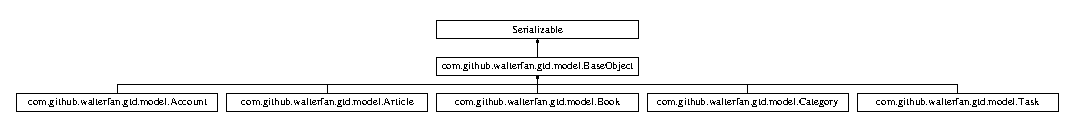
\includegraphics[height=1.272727cm]{classcom_1_1github_1_1walterfan_1_1gtd_1_1model_1_1BaseObject}
\end{center}
\end{figure}
\subsection*{Public Member Functions}
\begin{DoxyCompactItemize}
\item 
\hypertarget{classcom_1_1github_1_1walterfan_1_1gtd_1_1model_1_1BaseObject_af80a9f5d03ffbb1e2ad776b9d603401f}{boolean {\bfseries equals} (Object object)}\label{classcom_1_1github_1_1walterfan_1_1gtd_1_1model_1_1BaseObject_af80a9f5d03ffbb1e2ad776b9d603401f}

\item 
\hypertarget{classcom_1_1github_1_1walterfan_1_1gtd_1_1model_1_1BaseObject_a60edd102d3719adbe033d35402dc509c}{int {\bfseries hash\-Code} ()}\label{classcom_1_1github_1_1walterfan_1_1gtd_1_1model_1_1BaseObject_a60edd102d3719adbe033d35402dc509c}

\item 
\hypertarget{classcom_1_1github_1_1walterfan_1_1gtd_1_1model_1_1BaseObject_ab85b68e5efdce320dc5b1184d3d28d3c}{String {\bfseries to\-String} ()}\label{classcom_1_1github_1_1walterfan_1_1gtd_1_1model_1_1BaseObject_ab85b68e5efdce320dc5b1184d3d28d3c}

\item 
Object \hyperlink{classcom_1_1github_1_1walterfan_1_1gtd_1_1model_1_1BaseObject_aa9c242e5a1ff02058e26ddf277f56127}{get\-Field} (String str\-Field)  throws Illegal\-Access\-Exception,             Invocation\-Target\-Exception, No\-Such\-Method\-Exception 
\item 
Object \hyperlink{classcom_1_1github_1_1walterfan_1_1gtd_1_1model_1_1BaseObject_afa45970ded68ada4994d0a004c41275a}{invoke\-Method} (String str\-Method, Object...\-args)  throws Illegal\-Argument\-Exception, Illegal\-Access\-Exception,             Invocation\-Target\-Exception, Security\-Exception, No\-Such\-Method\-Exception 
\end{DoxyCompactItemize}
\subsection*{Protected Member Functions}
\begin{DoxyCompactItemize}
\item 
String \hyperlink{classcom_1_1github_1_1walterfan_1_1gtd_1_1model_1_1BaseObject_afbdf03e5477a44c75e95e6cc46a98d76}{read\-String} (Object\-Input in, int len)  throws I\-O\-Exception 
\item 
void \hyperlink{classcom_1_1github_1_1walterfan_1_1gtd_1_1model_1_1BaseObject_aa6dbf926bf2dea61bc4ae295c00c8998}{write\-String} (Object\-Output buf, String str)  throws I\-O\-Exception 
\end{DoxyCompactItemize}


\subsection{Detailed Description}
The Class \hyperlink{classcom_1_1github_1_1walterfan_1_1gtd_1_1model_1_1BaseObject}{Base\-Object}.

\begin{DoxyAuthor}{Author}
yafan 
\end{DoxyAuthor}


Definition at line 28 of file Base\-Object.\-java.



\subsection{Member Function Documentation}
\hypertarget{classcom_1_1github_1_1walterfan_1_1gtd_1_1model_1_1BaseObject_aa9c242e5a1ff02058e26ddf277f56127}{\index{com\-::github\-::walterfan\-::gtd\-::model\-::\-Base\-Object@{com\-::github\-::walterfan\-::gtd\-::model\-::\-Base\-Object}!get\-Field@{get\-Field}}
\index{get\-Field@{get\-Field}!com::github::walterfan::gtd::model::BaseObject@{com\-::github\-::walterfan\-::gtd\-::model\-::\-Base\-Object}}
\subsubsection[{get\-Field}]{\setlength{\rightskip}{0pt plus 5cm}Object com.\-github.\-walterfan.\-gtd.\-model.\-Base\-Object.\-get\-Field (
\begin{DoxyParamCaption}
\item[{String}]{str\-Field}
\end{DoxyParamCaption}
) throws Illegal\-Access\-Exception,             Invocation\-Target\-Exception, No\-Such\-Method\-Exception\hspace{0.3cm}{\ttfamily [inline]}}}\label{classcom_1_1github_1_1walterfan_1_1gtd_1_1model_1_1BaseObject_aa9c242e5a1ff02058e26ddf277f56127}
Gets the field.


\begin{DoxyParams}{Parameters}
{\em str\-Field} & the str field \\
\hline
\end{DoxyParams}
\begin{DoxyReturn}{Returns}
the field 
\end{DoxyReturn}

\begin{DoxyExceptions}{Exceptions}
{\em Illegal\-Access\-Exception} & the illegal access exception \\
\hline
{\em Invocation\-Target\-Exception} & the invocation target exception \\
\hline
{\em No\-Such\-Method\-Exception} & the no such method exception \\
\hline
\end{DoxyExceptions}


Definition at line 63 of file Base\-Object.\-java.


\begin{DoxyCode}
64                                                              \{
65         \textcolor{keywordflow}{return} PropertyUtils.getProperty(\textcolor{keyword}{this}, strField);
66     \}
\end{DoxyCode}
\hypertarget{classcom_1_1github_1_1walterfan_1_1gtd_1_1model_1_1BaseObject_afa45970ded68ada4994d0a004c41275a}{\index{com\-::github\-::walterfan\-::gtd\-::model\-::\-Base\-Object@{com\-::github\-::walterfan\-::gtd\-::model\-::\-Base\-Object}!invoke\-Method@{invoke\-Method}}
\index{invoke\-Method@{invoke\-Method}!com::github::walterfan::gtd::model::BaseObject@{com\-::github\-::walterfan\-::gtd\-::model\-::\-Base\-Object}}
\subsubsection[{invoke\-Method}]{\setlength{\rightskip}{0pt plus 5cm}Object com.\-github.\-walterfan.\-gtd.\-model.\-Base\-Object.\-invoke\-Method (
\begin{DoxyParamCaption}
\item[{String}]{str\-Method, }
\item[{Object...}]{args}
\end{DoxyParamCaption}
) throws Illegal\-Argument\-Exception, Illegal\-Access\-Exception,             Invocation\-Target\-Exception, Security\-Exception, No\-Such\-Method\-Exception\hspace{0.3cm}{\ttfamily [inline]}}}\label{classcom_1_1github_1_1walterfan_1_1gtd_1_1model_1_1BaseObject_afa45970ded68ada4994d0a004c41275a}
Invoke method.


\begin{DoxyParams}{Parameters}
{\em str\-Method} & the str method \\
\hline
{\em args} & the args \\
\hline
\end{DoxyParams}
\begin{DoxyReturn}{Returns}
the object 
\end{DoxyReturn}

\begin{DoxyExceptions}{Exceptions}
{\em Illegal\-Argument\-Exception} & the illegal argument exception \\
\hline
{\em Illegal\-Access\-Exception} & the illegal access exception \\
\hline
{\em Invocation\-Target\-Exception} & the invocation target exception \\
\hline
{\em Security\-Exception} & the security exception \\
\hline
{\em No\-Such\-Method\-Exception} & the no such method exception \\
\hline
\end{DoxyExceptions}


Definition at line 80 of file Base\-Object.\-java.


\begin{DoxyCode}
82                                                                                 \{
83         Method method = this.getClass().getMethod(strMethod, (Class<?>) null);
84         return method.invoke(this, args);
85     \}
\end{DoxyCode}
\hypertarget{classcom_1_1github_1_1walterfan_1_1gtd_1_1model_1_1BaseObject_afbdf03e5477a44c75e95e6cc46a98d76}{\index{com\-::github\-::walterfan\-::gtd\-::model\-::\-Base\-Object@{com\-::github\-::walterfan\-::gtd\-::model\-::\-Base\-Object}!read\-String@{read\-String}}
\index{read\-String@{read\-String}!com::github::walterfan::gtd::model::BaseObject@{com\-::github\-::walterfan\-::gtd\-::model\-::\-Base\-Object}}
\subsubsection[{read\-String}]{\setlength{\rightskip}{0pt plus 5cm}String com.\-github.\-walterfan.\-gtd.\-model.\-Base\-Object.\-read\-String (
\begin{DoxyParamCaption}
\item[{Object\-Input}]{in, }
\item[{int}]{len}
\end{DoxyParamCaption}
) throws I\-O\-Exception\hspace{0.3cm}{\ttfamily [inline]}, {\ttfamily [protected]}}}\label{classcom_1_1github_1_1walterfan_1_1gtd_1_1model_1_1BaseObject_afbdf03e5477a44c75e95e6cc46a98d76}
Read string.


\begin{DoxyParams}{Parameters}
{\em in} & the in \\
\hline
{\em len} & the len \\
\hline
\end{DoxyParams}
\begin{DoxyReturn}{Returns}
the string 
\end{DoxyReturn}

\begin{DoxyExceptions}{Exceptions}
{\em I\-O\-Exception} & Signals that an I/\-O exception has occurred. \\
\hline
\end{DoxyExceptions}


Definition at line 95 of file Base\-Object.\-java.


\begin{DoxyCode}
95                                                                             \{
96         \textcolor{keywordflow}{if} (len > 0) \{
97             byte[] bytes = \textcolor{keyword}{new} byte[len];
98             in.read(bytes, 0, len);
99             \textcolor{keywordflow}{return} \textcolor{keyword}{new} String(bytes);
100         \} \textcolor{keywordflow}{else} \{
101             \textcolor{keywordflow}{return} null;
102         \}
103     \}
\end{DoxyCode}
\hypertarget{classcom_1_1github_1_1walterfan_1_1gtd_1_1model_1_1BaseObject_aa6dbf926bf2dea61bc4ae295c00c8998}{\index{com\-::github\-::walterfan\-::gtd\-::model\-::\-Base\-Object@{com\-::github\-::walterfan\-::gtd\-::model\-::\-Base\-Object}!write\-String@{write\-String}}
\index{write\-String@{write\-String}!com::github::walterfan::gtd::model::BaseObject@{com\-::github\-::walterfan\-::gtd\-::model\-::\-Base\-Object}}
\subsubsection[{write\-String}]{\setlength{\rightskip}{0pt plus 5cm}void com.\-github.\-walterfan.\-gtd.\-model.\-Base\-Object.\-write\-String (
\begin{DoxyParamCaption}
\item[{Object\-Output}]{buf, }
\item[{String}]{str}
\end{DoxyParamCaption}
) throws I\-O\-Exception\hspace{0.3cm}{\ttfamily [inline]}, {\ttfamily [protected]}}}\label{classcom_1_1github_1_1walterfan_1_1gtd_1_1model_1_1BaseObject_aa6dbf926bf2dea61bc4ae295c00c8998}
Write string.


\begin{DoxyParams}{Parameters}
{\em buf} & the buf \\
\hline
{\em str} & the str \\
\hline
\end{DoxyParams}

\begin{DoxyExceptions}{Exceptions}
{\em I\-O\-Exception} & Signals that an I/\-O exception has occurred. \\
\hline
\end{DoxyExceptions}


Definition at line 112 of file Base\-Object.\-java.


\begin{DoxyCode}
112                                                                                 \{
113 
114         \textcolor{keywordflow}{if} (null == str) \{
115             buf.writeInt(0);
116         \} \textcolor{keywordflow}{else} \{
117             byte[] bytes = str.getBytes();
118             buf.writeInt(bytes.length);
119             buf.write(bytes);
120         \}
121     \}
\end{DoxyCode}


The documentation for this class was generated from the following file\-:\begin{DoxyCompactItemize}
\item 
/cygdrive/d/workspace/java/\-G\-T\-D/src/com/github/walterfan/gtd/model/Base\-Object.\-java\end{DoxyCompactItemize}

\hypertarget{classcom_1_1github_1_1walterfan_1_1gtd_1_1model_1_1Book}{\section{com.\-github.\-walterfan.\-gtd.\-model.\-Book Class Reference}
\label{classcom_1_1github_1_1walterfan_1_1gtd_1_1model_1_1Book}\index{com.\-github.\-walterfan.\-gtd.\-model.\-Book@{com.\-github.\-walterfan.\-gtd.\-model.\-Book}}
}
Inheritance diagram for com.\-github.\-walterfan.\-gtd.\-model.\-Book\-:\begin{figure}[H]
\begin{center}
\leavevmode
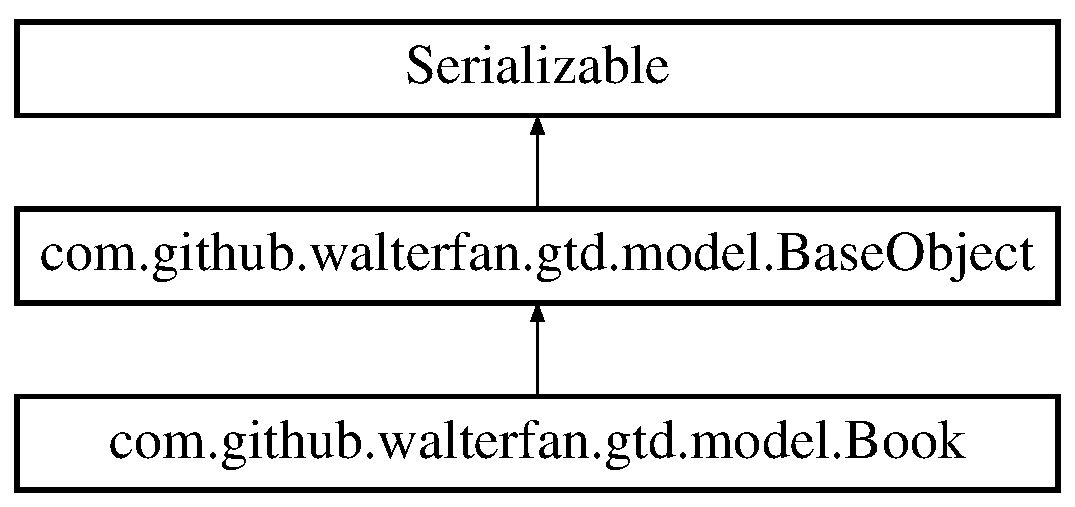
\includegraphics[height=3.000000cm]{classcom_1_1github_1_1walterfan_1_1gtd_1_1model_1_1Book}
\end{center}
\end{figure}
\subsection*{Public Member Functions}
\begin{DoxyCompactItemize}
\item 
\hypertarget{classcom_1_1github_1_1walterfan_1_1gtd_1_1model_1_1Book_aff2cefeba3872dbde6a8e141d0991207}{int {\bfseries get\-Book\-I\-D} ()}\label{classcom_1_1github_1_1walterfan_1_1gtd_1_1model_1_1Book_aff2cefeba3872dbde6a8e141d0991207}

\item 
\hypertarget{classcom_1_1github_1_1walterfan_1_1gtd_1_1model_1_1Book_a4199f5f14a3a839be5528880d0abf83e}{void {\bfseries set\-Book\-I\-D} (int book\-I\-D)}\label{classcom_1_1github_1_1walterfan_1_1gtd_1_1model_1_1Book_a4199f5f14a3a839be5528880d0abf83e}

\item 
\hypertarget{classcom_1_1github_1_1walterfan_1_1gtd_1_1model_1_1Book_ab267ae031a823c551732eada8f56b073}{String {\bfseries get\-Book\-S\-N} ()}\label{classcom_1_1github_1_1walterfan_1_1gtd_1_1model_1_1Book_ab267ae031a823c551732eada8f56b073}

\item 
\hypertarget{classcom_1_1github_1_1walterfan_1_1gtd_1_1model_1_1Book_a3d65e2c13fbede0a1a5b8c90d421e6a5}{void {\bfseries set\-Book\-S\-N} (String book\-S\-N)}\label{classcom_1_1github_1_1walterfan_1_1gtd_1_1model_1_1Book_a3d65e2c13fbede0a1a5b8c90d421e6a5}

\item 
\hypertarget{classcom_1_1github_1_1walterfan_1_1gtd_1_1model_1_1Book_aae7ee7e201af2f19cfb119d6de32428b}{String {\bfseries get\-Book\-Name} ()}\label{classcom_1_1github_1_1walterfan_1_1gtd_1_1model_1_1Book_aae7ee7e201af2f19cfb119d6de32428b}

\item 
\hypertarget{classcom_1_1github_1_1walterfan_1_1gtd_1_1model_1_1Book_a3c114cf174e1eb20de6f4a1ab005084a}{void {\bfseries set\-Book\-Name} (String book\-Name)}\label{classcom_1_1github_1_1walterfan_1_1gtd_1_1model_1_1Book_a3c114cf174e1eb20de6f4a1ab005084a}

\item 
\hypertarget{classcom_1_1github_1_1walterfan_1_1gtd_1_1model_1_1Book_a78519da0ed8470a18c71269994ea7c48}{int {\bfseries get\-Category\-I\-D} ()}\label{classcom_1_1github_1_1walterfan_1_1gtd_1_1model_1_1Book_a78519da0ed8470a18c71269994ea7c48}

\item 
\hypertarget{classcom_1_1github_1_1walterfan_1_1gtd_1_1model_1_1Book_a5917c9c56881d7cff1ee7279d68ef8e1}{void {\bfseries set\-Category\-I\-D} (int category\-I\-D)}\label{classcom_1_1github_1_1walterfan_1_1gtd_1_1model_1_1Book_a5917c9c56881d7cff1ee7279d68ef8e1}

\item 
\hypertarget{classcom_1_1github_1_1walterfan_1_1gtd_1_1model_1_1Book_ac04a62f9ed4c5a6f7af8bfd725716444}{Timestamp {\bfseries get\-Create\-Time} ()}\label{classcom_1_1github_1_1walterfan_1_1gtd_1_1model_1_1Book_ac04a62f9ed4c5a6f7af8bfd725716444}

\item 
\hypertarget{classcom_1_1github_1_1walterfan_1_1gtd_1_1model_1_1Book_a10a3dd297280764cf5c478fc3c279a80}{void {\bfseries set\-Create\-Time} (Timestamp create\-Time)}\label{classcom_1_1github_1_1walterfan_1_1gtd_1_1model_1_1Book_a10a3dd297280764cf5c478fc3c279a80}

\item 
\hypertarget{classcom_1_1github_1_1walterfan_1_1gtd_1_1model_1_1Book_a3e2ad7f1d3b7c4aa09f99f95b868c3e7}{String {\bfseries get\-Tags} ()}\label{classcom_1_1github_1_1walterfan_1_1gtd_1_1model_1_1Book_a3e2ad7f1d3b7c4aa09f99f95b868c3e7}

\item 
\hypertarget{classcom_1_1github_1_1walterfan_1_1gtd_1_1model_1_1Book_a9eeb2c631d09d9250cff4ec0b989ecb9}{void {\bfseries set\-Tags} (String tags)}\label{classcom_1_1github_1_1walterfan_1_1gtd_1_1model_1_1Book_a9eeb2c631d09d9250cff4ec0b989ecb9}

\item 
\hypertarget{classcom_1_1github_1_1walterfan_1_1gtd_1_1model_1_1Book_a6100304db75771c87a4b58b18b2b4ee4}{int {\bfseries get\-Borrow\-Log\-I\-D} ()}\label{classcom_1_1github_1_1walterfan_1_1gtd_1_1model_1_1Book_a6100304db75771c87a4b58b18b2b4ee4}

\item 
\hypertarget{classcom_1_1github_1_1walterfan_1_1gtd_1_1model_1_1Book_a2eaedd6b24e5b36590844c3b0676ad59}{void {\bfseries set\-Borrow\-Log\-I\-D} (int borrow\-Log\-I\-D)}\label{classcom_1_1github_1_1walterfan_1_1gtd_1_1model_1_1Book_a2eaedd6b24e5b36590844c3b0676ad59}

\end{DoxyCompactItemize}
\subsection*{Additional Inherited Members}


\subsection{Detailed Description}
\begin{DoxyAuthor}{Author}
walter 
\end{DoxyAuthor}


Definition at line 9 of file Book.\-java.



The documentation for this class was generated from the following file\-:\begin{DoxyCompactItemize}
\item 
/cygdrive/d/workspace/java/\-G\-T\-D/src/com/github/walterfan/gtd/model/Book.\-java\end{DoxyCompactItemize}

\hypertarget{classcom_1_1github_1_1walterfan_1_1gtd_1_1model_1_1Category}{\section{com.\-github.\-walterfan.\-gtd.\-model.\-Category Class Reference}
\label{classcom_1_1github_1_1walterfan_1_1gtd_1_1model_1_1Category}\index{com.\-github.\-walterfan.\-gtd.\-model.\-Category@{com.\-github.\-walterfan.\-gtd.\-model.\-Category}}
}
Inheritance diagram for com.\-github.\-walterfan.\-gtd.\-model.\-Category\-:\begin{figure}[H]
\begin{center}
\leavevmode
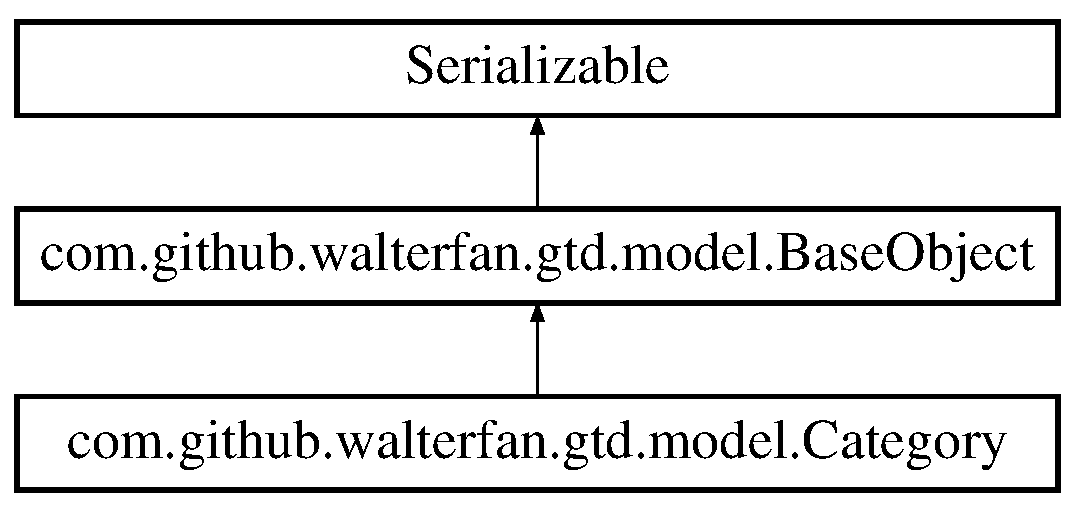
\includegraphics[height=3.000000cm]{classcom_1_1github_1_1walterfan_1_1gtd_1_1model_1_1Category}
\end{center}
\end{figure}
\subsection*{Public Member Functions}
\begin{DoxyCompactItemize}
\item 
\hypertarget{classcom_1_1github_1_1walterfan_1_1gtd_1_1model_1_1Category_a18942b853a1d8bf504946faf3ba08a5f}{{\bfseries Category} (String name)}\label{classcom_1_1github_1_1walterfan_1_1gtd_1_1model_1_1Category_a18942b853a1d8bf504946faf3ba08a5f}

\item 
\hypertarget{classcom_1_1github_1_1walterfan_1_1gtd_1_1model_1_1Category_a59722c593f0f672d68403d4807c73770}{Timestamp {\bfseries get\-Create\-Time} ()}\label{classcom_1_1github_1_1walterfan_1_1gtd_1_1model_1_1Category_a59722c593f0f672d68403d4807c73770}

\item 
\hypertarget{classcom_1_1github_1_1walterfan_1_1gtd_1_1model_1_1Category_a1cf4ad1a01734d72c48db8c19c9dbfa8}{void {\bfseries set\-Create\-Time} (Timestamp create\-Time)}\label{classcom_1_1github_1_1walterfan_1_1gtd_1_1model_1_1Category_a1cf4ad1a01734d72c48db8c19c9dbfa8}

\item 
int \hyperlink{classcom_1_1github_1_1walterfan_1_1gtd_1_1model_1_1Category_a8adbad441ee1eea37b2267c353a5dfee}{get\-Category\-I\-D} ()
\item 
void \hyperlink{classcom_1_1github_1_1walterfan_1_1gtd_1_1model_1_1Category_ae78e859ccb6928ac32efc3bd8e579a6c}{set\-Category\-I\-D} (int category\-I\-D)
\item 
String \hyperlink{classcom_1_1github_1_1walterfan_1_1gtd_1_1model_1_1Category_a015800eca4b86c7690ab1a49d31bc535}{get\-Category\-Name} ()
\item 
void \hyperlink{classcom_1_1github_1_1walterfan_1_1gtd_1_1model_1_1Category_a0b8da744bbf9242d26dec0de34aa0b51}{set\-Category\-Name} (String category\-Name)
\item 
String \hyperlink{classcom_1_1github_1_1walterfan_1_1gtd_1_1model_1_1Category_aa7fe1ebaf93a008f2631587b46271c80}{get\-Description} ()
\item 
void \hyperlink{classcom_1_1github_1_1walterfan_1_1gtd_1_1model_1_1Category_a022af1bf07d31d0234414456999cd7bf}{set\-Description} (String description)
\item 
int \hyperlink{classcom_1_1github_1_1walterfan_1_1gtd_1_1model_1_1Category_a286803b58064b17d53303362a15e6bc2}{get\-Category\-Type} ()
\item 
void \hyperlink{classcom_1_1github_1_1walterfan_1_1gtd_1_1model_1_1Category_a35cdbb1267d1703506754c47d60eb8a1}{set\-Category\-Type} (int category\-Type)
\end{DoxyCompactItemize}
\subsection*{Static Public Attributes}
\begin{DoxyCompactItemize}
\item 
\hypertarget{classcom_1_1github_1_1walterfan_1_1gtd_1_1model_1_1Category_ae30e233a23980f0299d7ffa8e562226b}{static final int {\bfseries C\-A\-T\-E\-G\-O\-R\-Y\-\_\-\-T\-Y\-P\-E\-\_\-\-T\-A\-S\-K} = 1}\label{classcom_1_1github_1_1walterfan_1_1gtd_1_1model_1_1Category_ae30e233a23980f0299d7ffa8e562226b}

\item 
\hypertarget{classcom_1_1github_1_1walterfan_1_1gtd_1_1model_1_1Category_a38a36ad79577bc1fd1d025fa09e5ff1c}{static final int {\bfseries C\-A\-T\-E\-G\-O\-R\-Y\-\_\-\-T\-Y\-P\-E\-\_\-\-L\-O\-R\-E} = 2}\label{classcom_1_1github_1_1walterfan_1_1gtd_1_1model_1_1Category_a38a36ad79577bc1fd1d025fa09e5ff1c}

\item 
\hypertarget{classcom_1_1github_1_1walterfan_1_1gtd_1_1model_1_1Category_a55c331913d0440d8b7c8fad74905b442}{static final int {\bfseries C\-A\-T\-E\-G\-O\-R\-Y\-\_\-\-T\-Y\-P\-E\-\_\-\-B\-O\-O\-K} = 3}\label{classcom_1_1github_1_1walterfan_1_1gtd_1_1model_1_1Category_a55c331913d0440d8b7c8fad74905b442}

\item 
\hypertarget{classcom_1_1github_1_1walterfan_1_1gtd_1_1model_1_1Category_aa766b7c2c2eed4870aa641a992b21afa}{static final int {\bfseries C\-A\-T\-E\-G\-O\-R\-Y\-\_\-\-T\-Y\-P\-E\-\_\-\-F\-R\-I\-E\-N\-D} = 4}\label{classcom_1_1github_1_1walterfan_1_1gtd_1_1model_1_1Category_aa766b7c2c2eed4870aa641a992b21afa}

\item 
\hypertarget{classcom_1_1github_1_1walterfan_1_1gtd_1_1model_1_1Category_abdd346424f44d02487dee9f7725b5da9}{static final int {\bfseries C\-A\-T\-E\-G\-O\-R\-Y\-\_\-\-T\-Y\-P\-E\-\_\-\-S\-I\-T\-E} = 5}\label{classcom_1_1github_1_1walterfan_1_1gtd_1_1model_1_1Category_abdd346424f44d02487dee9f7725b5da9}

\end{DoxyCompactItemize}
\subsection*{Additional Inherited Members}


\subsection{Detailed Description}
\begin{DoxyAuthor}{Author}
walter 
\end{DoxyAuthor}


Definition at line 9 of file Category.\-java.



\subsection{Member Function Documentation}
\hypertarget{classcom_1_1github_1_1walterfan_1_1gtd_1_1model_1_1Category_a8adbad441ee1eea37b2267c353a5dfee}{\index{com\-::github\-::walterfan\-::gtd\-::model\-::\-Category@{com\-::github\-::walterfan\-::gtd\-::model\-::\-Category}!get\-Category\-I\-D@{get\-Category\-I\-D}}
\index{get\-Category\-I\-D@{get\-Category\-I\-D}!com::github::walterfan::gtd::model::Category@{com\-::github\-::walterfan\-::gtd\-::model\-::\-Category}}
\subsubsection[{get\-Category\-I\-D}]{\setlength{\rightskip}{0pt plus 5cm}int com.\-github.\-walterfan.\-gtd.\-model.\-Category.\-get\-Category\-I\-D (
\begin{DoxyParamCaption}
{}
\end{DoxyParamCaption}
)\hspace{0.3cm}{\ttfamily [inline]}}}\label{classcom_1_1github_1_1walterfan_1_1gtd_1_1model_1_1Category_a8adbad441ee1eea37b2267c353a5dfee}
\begin{DoxyReturn}{Returns}
the category\-I\-D 
\end{DoxyReturn}


Definition at line 54 of file Category.\-java.


\begin{DoxyCode}
54                                \{
55         \textcolor{keywordflow}{return} categoryID;
56     \}
\end{DoxyCode}
\hypertarget{classcom_1_1github_1_1walterfan_1_1gtd_1_1model_1_1Category_a015800eca4b86c7690ab1a49d31bc535}{\index{com\-::github\-::walterfan\-::gtd\-::model\-::\-Category@{com\-::github\-::walterfan\-::gtd\-::model\-::\-Category}!get\-Category\-Name@{get\-Category\-Name}}
\index{get\-Category\-Name@{get\-Category\-Name}!com::github::walterfan::gtd::model::Category@{com\-::github\-::walterfan\-::gtd\-::model\-::\-Category}}
\subsubsection[{get\-Category\-Name}]{\setlength{\rightskip}{0pt plus 5cm}String com.\-github.\-walterfan.\-gtd.\-model.\-Category.\-get\-Category\-Name (
\begin{DoxyParamCaption}
{}
\end{DoxyParamCaption}
)\hspace{0.3cm}{\ttfamily [inline]}}}\label{classcom_1_1github_1_1walterfan_1_1gtd_1_1model_1_1Category_a015800eca4b86c7690ab1a49d31bc535}
\begin{DoxyReturn}{Returns}
the category\-Name 
\end{DoxyReturn}


Definition at line 69 of file Category.\-java.


\begin{DoxyCode}
69                                     \{
70         \textcolor{keywordflow}{return} categoryName;
71     \}
\end{DoxyCode}
\hypertarget{classcom_1_1github_1_1walterfan_1_1gtd_1_1model_1_1Category_a286803b58064b17d53303362a15e6bc2}{\index{com\-::github\-::walterfan\-::gtd\-::model\-::\-Category@{com\-::github\-::walterfan\-::gtd\-::model\-::\-Category}!get\-Category\-Type@{get\-Category\-Type}}
\index{get\-Category\-Type@{get\-Category\-Type}!com::github::walterfan::gtd::model::Category@{com\-::github\-::walterfan\-::gtd\-::model\-::\-Category}}
\subsubsection[{get\-Category\-Type}]{\setlength{\rightskip}{0pt plus 5cm}int com.\-github.\-walterfan.\-gtd.\-model.\-Category.\-get\-Category\-Type (
\begin{DoxyParamCaption}
{}
\end{DoxyParamCaption}
)\hspace{0.3cm}{\ttfamily [inline]}}}\label{classcom_1_1github_1_1walterfan_1_1gtd_1_1model_1_1Category_a286803b58064b17d53303362a15e6bc2}
\begin{DoxyReturn}{Returns}
the category\-Type 
\end{DoxyReturn}


Definition at line 99 of file Category.\-java.


\begin{DoxyCode}
99                                  \{
100         \textcolor{keywordflow}{return} categoryType;
101     \}
\end{DoxyCode}
\hypertarget{classcom_1_1github_1_1walterfan_1_1gtd_1_1model_1_1Category_aa7fe1ebaf93a008f2631587b46271c80}{\index{com\-::github\-::walterfan\-::gtd\-::model\-::\-Category@{com\-::github\-::walterfan\-::gtd\-::model\-::\-Category}!get\-Description@{get\-Description}}
\index{get\-Description@{get\-Description}!com::github::walterfan::gtd::model::Category@{com\-::github\-::walterfan\-::gtd\-::model\-::\-Category}}
\subsubsection[{get\-Description}]{\setlength{\rightskip}{0pt plus 5cm}String com.\-github.\-walterfan.\-gtd.\-model.\-Category.\-get\-Description (
\begin{DoxyParamCaption}
{}
\end{DoxyParamCaption}
)\hspace{0.3cm}{\ttfamily [inline]}}}\label{classcom_1_1github_1_1walterfan_1_1gtd_1_1model_1_1Category_aa7fe1ebaf93a008f2631587b46271c80}
\begin{DoxyReturn}{Returns}
the description 
\end{DoxyReturn}


Definition at line 84 of file Category.\-java.


\begin{DoxyCode}
84                                    \{
85         \textcolor{keywordflow}{return} description;
86     \}
\end{DoxyCode}
\hypertarget{classcom_1_1github_1_1walterfan_1_1gtd_1_1model_1_1Category_ae78e859ccb6928ac32efc3bd8e579a6c}{\index{com\-::github\-::walterfan\-::gtd\-::model\-::\-Category@{com\-::github\-::walterfan\-::gtd\-::model\-::\-Category}!set\-Category\-I\-D@{set\-Category\-I\-D}}
\index{set\-Category\-I\-D@{set\-Category\-I\-D}!com::github::walterfan::gtd::model::Category@{com\-::github\-::walterfan\-::gtd\-::model\-::\-Category}}
\subsubsection[{set\-Category\-I\-D}]{\setlength{\rightskip}{0pt plus 5cm}void com.\-github.\-walterfan.\-gtd.\-model.\-Category.\-set\-Category\-I\-D (
\begin{DoxyParamCaption}
\item[{int}]{category\-I\-D}
\end{DoxyParamCaption}
)\hspace{0.3cm}{\ttfamily [inline]}}}\label{classcom_1_1github_1_1walterfan_1_1gtd_1_1model_1_1Category_ae78e859ccb6928ac32efc3bd8e579a6c}

\begin{DoxyParams}{Parameters}
{\em category\-I\-D} & the category\-I\-D to set \\
\hline
\end{DoxyParams}


Definition at line 62 of file Category.\-java.


\begin{DoxyCode}
62                                               \{
63         this.categoryID = categoryID;
64     \}
\end{DoxyCode}
\hypertarget{classcom_1_1github_1_1walterfan_1_1gtd_1_1model_1_1Category_a0b8da744bbf9242d26dec0de34aa0b51}{\index{com\-::github\-::walterfan\-::gtd\-::model\-::\-Category@{com\-::github\-::walterfan\-::gtd\-::model\-::\-Category}!set\-Category\-Name@{set\-Category\-Name}}
\index{set\-Category\-Name@{set\-Category\-Name}!com::github::walterfan::gtd::model::Category@{com\-::github\-::walterfan\-::gtd\-::model\-::\-Category}}
\subsubsection[{set\-Category\-Name}]{\setlength{\rightskip}{0pt plus 5cm}void com.\-github.\-walterfan.\-gtd.\-model.\-Category.\-set\-Category\-Name (
\begin{DoxyParamCaption}
\item[{String}]{category\-Name}
\end{DoxyParamCaption}
)\hspace{0.3cm}{\ttfamily [inline]}}}\label{classcom_1_1github_1_1walterfan_1_1gtd_1_1model_1_1Category_a0b8da744bbf9242d26dec0de34aa0b51}

\begin{DoxyParams}{Parameters}
{\em category\-Name} & the category\-Name to set \\
\hline
\end{DoxyParams}


Definition at line 77 of file Category.\-java.


\begin{DoxyCode}
77                                                      \{
78         this.categoryName = categoryName;
79     \}
\end{DoxyCode}
\hypertarget{classcom_1_1github_1_1walterfan_1_1gtd_1_1model_1_1Category_a35cdbb1267d1703506754c47d60eb8a1}{\index{com\-::github\-::walterfan\-::gtd\-::model\-::\-Category@{com\-::github\-::walterfan\-::gtd\-::model\-::\-Category}!set\-Category\-Type@{set\-Category\-Type}}
\index{set\-Category\-Type@{set\-Category\-Type}!com::github::walterfan::gtd::model::Category@{com\-::github\-::walterfan\-::gtd\-::model\-::\-Category}}
\subsubsection[{set\-Category\-Type}]{\setlength{\rightskip}{0pt plus 5cm}void com.\-github.\-walterfan.\-gtd.\-model.\-Category.\-set\-Category\-Type (
\begin{DoxyParamCaption}
\item[{int}]{category\-Type}
\end{DoxyParamCaption}
)\hspace{0.3cm}{\ttfamily [inline]}}}\label{classcom_1_1github_1_1walterfan_1_1gtd_1_1model_1_1Category_a35cdbb1267d1703506754c47d60eb8a1}

\begin{DoxyParams}{Parameters}
{\em category\-Type} & the category\-Type to set \\
\hline
\end{DoxyParams}


Definition at line 107 of file Category.\-java.


\begin{DoxyCode}
107                                                   \{
108         this.categoryType = categoryType;
109     \}
\end{DoxyCode}
\hypertarget{classcom_1_1github_1_1walterfan_1_1gtd_1_1model_1_1Category_a022af1bf07d31d0234414456999cd7bf}{\index{com\-::github\-::walterfan\-::gtd\-::model\-::\-Category@{com\-::github\-::walterfan\-::gtd\-::model\-::\-Category}!set\-Description@{set\-Description}}
\index{set\-Description@{set\-Description}!com::github::walterfan::gtd::model::Category@{com\-::github\-::walterfan\-::gtd\-::model\-::\-Category}}
\subsubsection[{set\-Description}]{\setlength{\rightskip}{0pt plus 5cm}void com.\-github.\-walterfan.\-gtd.\-model.\-Category.\-set\-Description (
\begin{DoxyParamCaption}
\item[{String}]{description}
\end{DoxyParamCaption}
)\hspace{0.3cm}{\ttfamily [inline]}}}\label{classcom_1_1github_1_1walterfan_1_1gtd_1_1model_1_1Category_a022af1bf07d31d0234414456999cd7bf}

\begin{DoxyParams}{Parameters}
{\em description} & the description to set \\
\hline
\end{DoxyParams}


Definition at line 92 of file Category.\-java.


\begin{DoxyCode}
92                                                    \{
93         this.description = description;
94     \}
\end{DoxyCode}


The documentation for this class was generated from the following file\-:\begin{DoxyCompactItemize}
\item 
/cygdrive/d/workspace/java/\-G\-T\-D/src/com/github/walterfan/gtd/model/Category.\-java\end{DoxyCompactItemize}

\hypertarget{classcom_1_1github_1_1walterfan_1_1gtd_1_1ui_1_1ConfirmDialogFragment}{\section{com.\-github.\-walterfan.\-gtd.\-ui.\-Confirm\-Dialog\-Fragment Class Reference}
\label{classcom_1_1github_1_1walterfan_1_1gtd_1_1ui_1_1ConfirmDialogFragment}\index{com.\-github.\-walterfan.\-gtd.\-ui.\-Confirm\-Dialog\-Fragment@{com.\-github.\-walterfan.\-gtd.\-ui.\-Confirm\-Dialog\-Fragment}}
}
Inheritance diagram for com.\-github.\-walterfan.\-gtd.\-ui.\-Confirm\-Dialog\-Fragment\-:\begin{figure}[H]
\begin{center}
\leavevmode
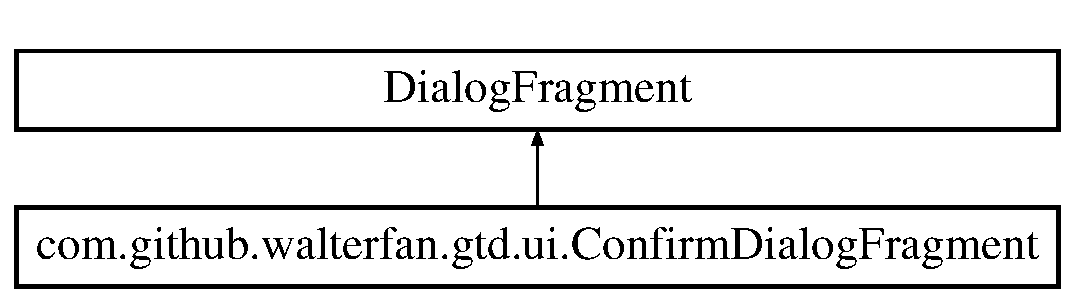
\includegraphics[height=2.000000cm]{classcom_1_1github_1_1walterfan_1_1gtd_1_1ui_1_1ConfirmDialogFragment}
\end{center}
\end{figure}
\subsection*{Public Member Functions}
\begin{DoxyCompactItemize}
\item 
\hypertarget{classcom_1_1github_1_1walterfan_1_1gtd_1_1ui_1_1ConfirmDialogFragment_a49ee392acba07a2ac605a60787aa5b89}{Dialog\-Interface.\-On\-Click\-Listener {\bfseries get\-Okay\-Listener} ()}\label{classcom_1_1github_1_1walterfan_1_1gtd_1_1ui_1_1ConfirmDialogFragment_a49ee392acba07a2ac605a60787aa5b89}

\item 
\hypertarget{classcom_1_1github_1_1walterfan_1_1gtd_1_1ui_1_1ConfirmDialogFragment_a41e71fc2203cc8ee0a2d1826f5e610d0}{void {\bfseries set\-Okay\-Listener} (Dialog\-Interface.\-On\-Click\-Listener okay\-Listener)}\label{classcom_1_1github_1_1walterfan_1_1gtd_1_1ui_1_1ConfirmDialogFragment_a41e71fc2203cc8ee0a2d1826f5e610d0}

\item 
\hypertarget{classcom_1_1github_1_1walterfan_1_1gtd_1_1ui_1_1ConfirmDialogFragment_ab74ad966b344b1f6dab9b77e6cbc807d}{Dialog\-Interface.\-On\-Click\-Listener {\bfseries get\-Cancel\-Listener} ()}\label{classcom_1_1github_1_1walterfan_1_1gtd_1_1ui_1_1ConfirmDialogFragment_ab74ad966b344b1f6dab9b77e6cbc807d}

\item 
\hypertarget{classcom_1_1github_1_1walterfan_1_1gtd_1_1ui_1_1ConfirmDialogFragment_a5607267202db07d68de5cc273ddcb9b8}{void {\bfseries set\-Cancel\-Listener} (Dialog\-Interface.\-On\-Click\-Listener cancel\-Listener)}\label{classcom_1_1github_1_1walterfan_1_1gtd_1_1ui_1_1ConfirmDialogFragment_a5607267202db07d68de5cc273ddcb9b8}

\item 
\hypertarget{classcom_1_1github_1_1walterfan_1_1gtd_1_1ui_1_1ConfirmDialogFragment_a3c0de676c53990e4e7f4a50ddbc4ffad}{Dialog {\bfseries on\-Create\-Dialog} (Bundle saved\-Instance\-State)}\label{classcom_1_1github_1_1walterfan_1_1gtd_1_1ui_1_1ConfirmDialogFragment_a3c0de676c53990e4e7f4a50ddbc4ffad}

\end{DoxyCompactItemize}


\subsection{Detailed Description}


Definition at line 12 of file Confirm\-Dialog\-Fragment.\-java.



The documentation for this class was generated from the following file\-:\begin{DoxyCompactItemize}
\item 
/cygdrive/d/workspace/java/\-G\-T\-D/src/com/github/walterfan/gtd/ui/Confirm\-Dialog\-Fragment.\-java\end{DoxyCompactItemize}

\hypertarget{classwfan_1_1CSubject}{\section{wfan\-:\-:C\-Subject Class Reference}
\label{classwfan_1_1CSubject}\index{wfan\-::\-C\-Subject@{wfan\-::\-C\-Subject}}
}
Inheritance diagram for wfan\-:\-:C\-Subject\-:\begin{figure}[H]
\begin{center}
\leavevmode
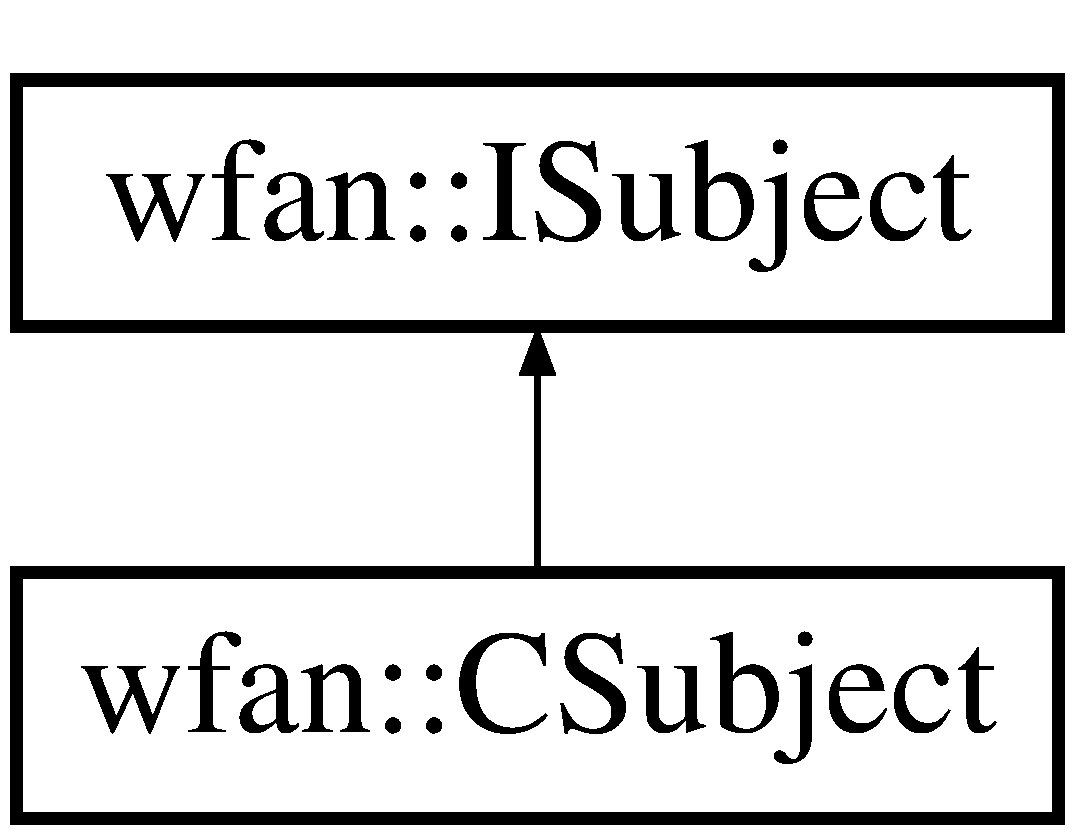
\includegraphics[height=2.000000cm]{classwfan_1_1CSubject}
\end{center}
\end{figure}
\subsection*{Public Member Functions}
\begin{DoxyCompactItemize}
\item 
\hypertarget{classwfan_1_1CSubject_add6003a736e35f618c8d8777cfdaab0b}{virtual void {\bfseries Attach} (\hyperlink{classwfan_1_1IObserver}{I\-Observer} $\ast$p\-Observer)}\label{classwfan_1_1CSubject_add6003a736e35f618c8d8777cfdaab0b}

\item 
\hypertarget{classwfan_1_1CSubject_a1f37b4c07b0321e4bf0272cea120ca6f}{virtual void {\bfseries Detach} (\hyperlink{classwfan_1_1IObserver}{I\-Observer} $\ast$p\-Observer)}\label{classwfan_1_1CSubject_a1f37b4c07b0321e4bf0272cea120ca6f}

\item 
\hypertarget{classwfan_1_1CSubject_a4bd9c19bf9af8d0f49b88f969b185ad5}{virtual void {\bfseries Notify} ()}\label{classwfan_1_1CSubject_a4bd9c19bf9af8d0f49b88f969b185ad5}

\end{DoxyCompactItemize}


\subsection{Detailed Description}


Definition at line 50 of file Observer.\-h.



The documentation for this class was generated from the following files\-:\begin{DoxyCompactItemize}
\item 
/cygdrive/d/workspace/java/\-G\-T\-D/jni/util/Observer.\-h\item 
/cygdrive/d/workspace/java/\-G\-T\-D/jni/util/Observer.\-cpp\end{DoxyCompactItemize}

\hypertarget{classcom_1_1github_1_1walterfan_1_1gtd_1_1service_1_1DataSyncService}{\section{com.\-github.\-walterfan.\-gtd.\-service.\-Data\-Sync\-Service Class Reference}
\label{classcom_1_1github_1_1walterfan_1_1gtd_1_1service_1_1DataSyncService}\index{com.\-github.\-walterfan.\-gtd.\-service.\-Data\-Sync\-Service@{com.\-github.\-walterfan.\-gtd.\-service.\-Data\-Sync\-Service}}
}
Inheritance diagram for com.\-github.\-walterfan.\-gtd.\-service.\-Data\-Sync\-Service\-:\begin{figure}[H]
\begin{center}
\leavevmode
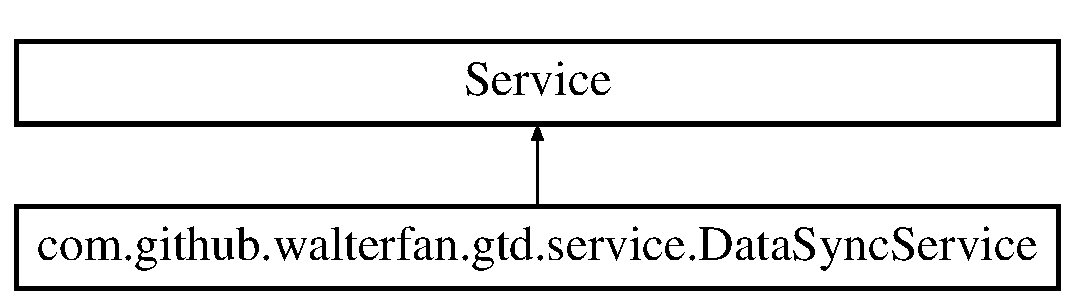
\includegraphics[height=2.000000cm]{classcom_1_1github_1_1walterfan_1_1gtd_1_1service_1_1DataSyncService}
\end{center}
\end{figure}
\subsection*{Classes}
\begin{DoxyCompactItemize}
\item 
class \hyperlink{classcom_1_1github_1_1walterfan_1_1gtd_1_1service_1_1DataSyncService_1_1ServiceCountBinder}{Service\-Count\-Binder}
\end{DoxyCompactItemize}
\subsection*{Public Member Functions}
\begin{DoxyCompactItemize}
\item 
\hypertarget{classcom_1_1github_1_1walterfan_1_1gtd_1_1service_1_1DataSyncService_a8a5f6bde4dde48a134c4999cc013c5bb}{I\-Binder {\bfseries on\-Bind} (Intent arg0)}\label{classcom_1_1github_1_1walterfan_1_1gtd_1_1service_1_1DataSyncService_a8a5f6bde4dde48a134c4999cc013c5bb}

\item 
\hypertarget{classcom_1_1github_1_1walterfan_1_1gtd_1_1service_1_1DataSyncService_a66f5926a213663cd6163e12bbab8d5ed}{boolean {\bfseries on\-Unbind} (Intent intent)}\label{classcom_1_1github_1_1walterfan_1_1gtd_1_1service_1_1DataSyncService_a66f5926a213663cd6163e12bbab8d5ed}

\item 
\hypertarget{classcom_1_1github_1_1walterfan_1_1gtd_1_1service_1_1DataSyncService_a897e80cde7e29e8aaf93a8da8322672e}{void {\bfseries on\-Create} ()}\label{classcom_1_1github_1_1walterfan_1_1gtd_1_1service_1_1DataSyncService_a897e80cde7e29e8aaf93a8da8322672e}

\item 
\hypertarget{classcom_1_1github_1_1walterfan_1_1gtd_1_1service_1_1DataSyncService_ac3af94077f6301e227828eaddabd7f80}{void {\bfseries on\-Start} (Intent intent, int start\-Id)}\label{classcom_1_1github_1_1walterfan_1_1gtd_1_1service_1_1DataSyncService_ac3af94077f6301e227828eaddabd7f80}

\item 
\hypertarget{classcom_1_1github_1_1walterfan_1_1gtd_1_1service_1_1DataSyncService_a6200c5384d706dc582e69547037b2b7c}{void {\bfseries on\-Destroy} ()}\label{classcom_1_1github_1_1walterfan_1_1gtd_1_1service_1_1DataSyncService_a6200c5384d706dc582e69547037b2b7c}

\end{DoxyCompactItemize}


\subsection{Detailed Description}


Definition at line 9 of file Data\-Sync\-Service.\-java.



The documentation for this class was generated from the following file\-:\begin{DoxyCompactItemize}
\item 
/cygdrive/d/workspace/java/\-G\-T\-D/src/com/github/walterfan/gtd/service/Data\-Sync\-Service.\-java\end{DoxyCompactItemize}

\hypertarget{classcom_1_1github_1_1walterfan_1_1gtd_1_1test_1_1DialogTest}{\section{com.\-github.\-walterfan.\-gtd.\-test.\-Dialog\-Test Class Reference}
\label{classcom_1_1github_1_1walterfan_1_1gtd_1_1test_1_1DialogTest}\index{com.\-github.\-walterfan.\-gtd.\-test.\-Dialog\-Test@{com.\-github.\-walterfan.\-gtd.\-test.\-Dialog\-Test}}
}
Inheritance diagram for com.\-github.\-walterfan.\-gtd.\-test.\-Dialog\-Test\-:\begin{figure}[H]
\begin{center}
\leavevmode
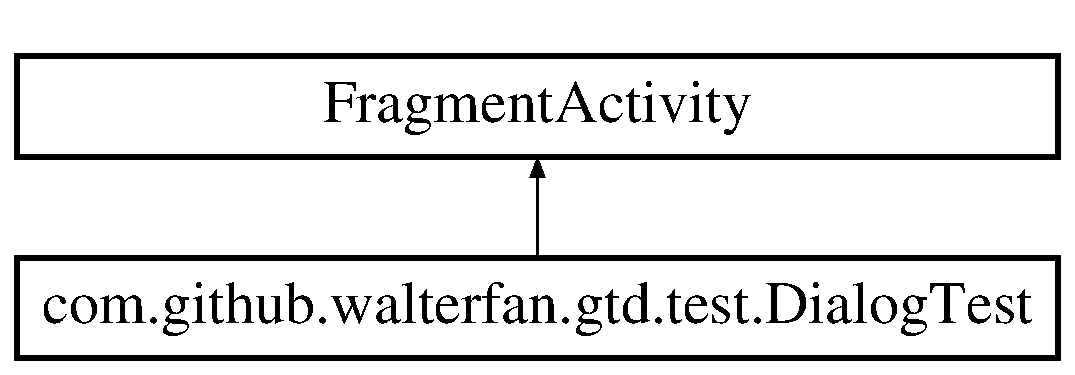
\includegraphics[height=2.000000cm]{classcom_1_1github_1_1walterfan_1_1gtd_1_1test_1_1DialogTest}
\end{center}
\end{figure}
\subsection*{Public Member Functions}
\begin{DoxyCompactItemize}
\item 
\hypertarget{classcom_1_1github_1_1walterfan_1_1gtd_1_1test_1_1DialogTest_ae3af60ec806b2496db140edd17b4d317}{void {\bfseries show\-Confirm\-Dialog} ()}\label{classcom_1_1github_1_1walterfan_1_1gtd_1_1test_1_1DialogTest_ae3af60ec806b2496db140edd17b4d317}

\end{DoxyCompactItemize}
\subsection*{Protected Member Functions}
\begin{DoxyCompactItemize}
\item 
\hypertarget{classcom_1_1github_1_1walterfan_1_1gtd_1_1test_1_1DialogTest_ae8c44d70382323681fc11fa5b65ad3c6}{void {\bfseries on\-Create} (Bundle saved\-Instance\-State)}\label{classcom_1_1github_1_1walterfan_1_1gtd_1_1test_1_1DialogTest_ae8c44d70382323681fc11fa5b65ad3c6}

\end{DoxyCompactItemize}


\subsection{Detailed Description}


Definition at line 14 of file Dialog\-Test.\-java.



The documentation for this class was generated from the following file\-:\begin{DoxyCompactItemize}
\item 
/cygdrive/d/workspace/java/\-G\-T\-D/src/com/github/walterfan/gtd/test/Dialog\-Test.\-java\end{DoxyCompactItemize}

\hypertarget{classcom_1_1github_1_1walterfan_1_1gtd_1_1ui_1_1DisplayMessageActivity}{\section{com.\-github.\-walterfan.\-gtd.\-ui.\-Display\-Message\-Activity Class Reference}
\label{classcom_1_1github_1_1walterfan_1_1gtd_1_1ui_1_1DisplayMessageActivity}\index{com.\-github.\-walterfan.\-gtd.\-ui.\-Display\-Message\-Activity@{com.\-github.\-walterfan.\-gtd.\-ui.\-Display\-Message\-Activity}}
}
Inheritance diagram for com.\-github.\-walterfan.\-gtd.\-ui.\-Display\-Message\-Activity\-:\begin{figure}[H]
\begin{center}
\leavevmode
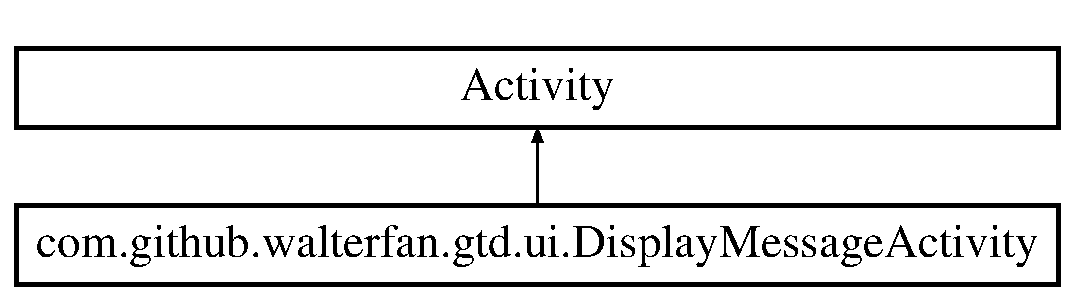
\includegraphics[height=2.000000cm]{classcom_1_1github_1_1walterfan_1_1gtd_1_1ui_1_1DisplayMessageActivity}
\end{center}
\end{figure}
\subsection*{Public Member Functions}
\begin{DoxyCompactItemize}
\item 
\hypertarget{classcom_1_1github_1_1walterfan_1_1gtd_1_1ui_1_1DisplayMessageActivity_a12f5742662e3bd6169473e735c47fd37}{void {\bfseries on\-Create} (Bundle saved\-Instance\-State)}\label{classcom_1_1github_1_1walterfan_1_1gtd_1_1ui_1_1DisplayMessageActivity_a12f5742662e3bd6169473e735c47fd37}

\item 
\hypertarget{classcom_1_1github_1_1walterfan_1_1gtd_1_1ui_1_1DisplayMessageActivity_a41ccaf42379e4210855749e6954dc5ed}{boolean {\bfseries on\-Options\-Item\-Selected} (Menu\-Item item)}\label{classcom_1_1github_1_1walterfan_1_1gtd_1_1ui_1_1DisplayMessageActivity_a41ccaf42379e4210855749e6954dc5ed}

\end{DoxyCompactItemize}


\subsection{Detailed Description}


Definition at line 12 of file Display\-Message\-Activity.\-java.



The documentation for this class was generated from the following file\-:\begin{DoxyCompactItemize}
\item 
/cygdrive/d/workspace/java/\-G\-T\-D/src/com/github/walterfan/gtd/ui/Display\-Message\-Activity.\-java\end{DoxyCompactItemize}

\hypertarget{interfacecom_1_1github_1_1walterfan_1_1gtd_1_1game_1_1FileIO}{\section{com.\-github.\-walterfan.\-gtd.\-game.\-File\-I\-O Interface Reference}
\label{interfacecom_1_1github_1_1walterfan_1_1gtd_1_1game_1_1FileIO}\index{com.\-github.\-walterfan.\-gtd.\-game.\-File\-I\-O@{com.\-github.\-walterfan.\-gtd.\-game.\-File\-I\-O}}
}
\subsection*{Public Member Functions}
\begin{DoxyCompactItemize}
\item 
\hypertarget{interfacecom_1_1github_1_1walterfan_1_1gtd_1_1game_1_1FileIO_a3eb8893b906361c330f344ee1c0eaba2}{Input\-Stream {\bfseries read\-Asset} (String filename)  throws I\-O\-Exception}\label{interfacecom_1_1github_1_1walterfan_1_1gtd_1_1game_1_1FileIO_a3eb8893b906361c330f344ee1c0eaba2}

\item 
\hypertarget{interfacecom_1_1github_1_1walterfan_1_1gtd_1_1game_1_1FileIO_ad449722240921b984c5c06eec3832dad}{Input\-Stream {\bfseries read\-File} (String filename)  throws I\-O\-Exception}\label{interfacecom_1_1github_1_1walterfan_1_1gtd_1_1game_1_1FileIO_ad449722240921b984c5c06eec3832dad}

\item 
\hypertarget{interfacecom_1_1github_1_1walterfan_1_1gtd_1_1game_1_1FileIO_a8ac6636889400e2f89fb70756bd32759}{Output\-Stream {\bfseries write\-File} (String filename)  throws I\-O\-Exception}\label{interfacecom_1_1github_1_1walterfan_1_1gtd_1_1game_1_1FileIO_a8ac6636889400e2f89fb70756bd32759}

\end{DoxyCompactItemize}


\subsection{Detailed Description}


Definition at line 7 of file File\-I\-O.\-java.



The documentation for this interface was generated from the following file\-:\begin{DoxyCompactItemize}
\item 
/cygdrive/d/workspace/java/\-G\-T\-D/src/com/github/walterfan/gtd/game/File\-I\-O.\-java\end{DoxyCompactItemize}

\hypertarget{interfacecom_1_1github_1_1walterfan_1_1gtd_1_1game_1_1Game}{\section{com.\-github.\-walterfan.\-gtd.\-game.\-Game Interface Reference}
\label{interfacecom_1_1github_1_1walterfan_1_1gtd_1_1game_1_1Game}\index{com.\-github.\-walterfan.\-gtd.\-game.\-Game@{com.\-github.\-walterfan.\-gtd.\-game.\-Game}}
}
\subsection*{Public Member Functions}
\begin{DoxyCompactItemize}
\item 
\hypertarget{interfacecom_1_1github_1_1walterfan_1_1gtd_1_1game_1_1Game_a8223a3d81fd2cea0ed4cee4a4df11513}{\hyperlink{interfacecom_1_1github_1_1walterfan_1_1gtd_1_1game_1_1Input}{Input} {\bfseries get\-Input} ()}\label{interfacecom_1_1github_1_1walterfan_1_1gtd_1_1game_1_1Game_a8223a3d81fd2cea0ed4cee4a4df11513}

\item 
\hypertarget{interfacecom_1_1github_1_1walterfan_1_1gtd_1_1game_1_1Game_ac99ccf06e5a691b3a9192039951815d3}{\hyperlink{interfacecom_1_1github_1_1walterfan_1_1gtd_1_1game_1_1FileIO}{File\-I\-O} {\bfseries get\-File\-I\-O} ()}\label{interfacecom_1_1github_1_1walterfan_1_1gtd_1_1game_1_1Game_ac99ccf06e5a691b3a9192039951815d3}

\item 
\hypertarget{interfacecom_1_1github_1_1walterfan_1_1gtd_1_1game_1_1Game_afe089a82f3bfa3e3ea96c21c34996e09}{\hyperlink{interfacecom_1_1github_1_1walterfan_1_1gtd_1_1game_1_1Graphics}{Graphics} {\bfseries get\-Graphics} ()}\label{interfacecom_1_1github_1_1walterfan_1_1gtd_1_1game_1_1Game_afe089a82f3bfa3e3ea96c21c34996e09}

\item 
\hypertarget{interfacecom_1_1github_1_1walterfan_1_1gtd_1_1game_1_1Game_ade4d723432221e8867fcb1dda1200f99}{\hyperlink{classcom_1_1github_1_1walterfan_1_1gtd_1_1game_1_1Audio}{Audio} {\bfseries get\-Audio} ()}\label{interfacecom_1_1github_1_1walterfan_1_1gtd_1_1game_1_1Game_ade4d723432221e8867fcb1dda1200f99}

\item 
\hypertarget{interfacecom_1_1github_1_1walterfan_1_1gtd_1_1game_1_1Game_adad8888340f01d72f3efdfc57debcf69}{void {\bfseries set\-Screen} (\hyperlink{classcom_1_1github_1_1walterfan_1_1gtd_1_1game_1_1Screen}{Screen} screen)}\label{interfacecom_1_1github_1_1walterfan_1_1gtd_1_1game_1_1Game_adad8888340f01d72f3efdfc57debcf69}

\item 
\hypertarget{interfacecom_1_1github_1_1walterfan_1_1gtd_1_1game_1_1Game_ae1fb8cc40d82033e2ac888ba86dff966}{\hyperlink{classcom_1_1github_1_1walterfan_1_1gtd_1_1game_1_1Screen}{Screen} {\bfseries get\-Current\-Screen} ()}\label{interfacecom_1_1github_1_1walterfan_1_1gtd_1_1game_1_1Game_ae1fb8cc40d82033e2ac888ba86dff966}

\item 
\hypertarget{interfacecom_1_1github_1_1walterfan_1_1gtd_1_1game_1_1Game_a0ef484d6ccd07086dbedb14e0d441116}{\hyperlink{classcom_1_1github_1_1walterfan_1_1gtd_1_1game_1_1Screen}{Screen} {\bfseries get\-Start\-Screen} ()}\label{interfacecom_1_1github_1_1walterfan_1_1gtd_1_1game_1_1Game_a0ef484d6ccd07086dbedb14e0d441116}

\end{DoxyCompactItemize}


\subsection{Detailed Description}


Definition at line 3 of file Game.\-java.



The documentation for this interface was generated from the following file\-:\begin{DoxyCompactItemize}
\item 
/cygdrive/d/workspace/java/\-G\-T\-D/src/com/github/walterfan/gtd/game/Game.\-java\end{DoxyCompactItemize}

\hypertarget{interfacecom_1_1github_1_1walterfan_1_1gtd_1_1game_1_1Graphics}{\section{com.\-github.\-walterfan.\-gtd.\-game.\-Graphics Interface Reference}
\label{interfacecom_1_1github_1_1walterfan_1_1gtd_1_1game_1_1Graphics}\index{com.\-github.\-walterfan.\-gtd.\-game.\-Graphics@{com.\-github.\-walterfan.\-gtd.\-game.\-Graphics}}
}
\subsection*{Classes}
\begin{DoxyCompactItemize}
\item 
enum {\bfseries Pixmap\-Format}
\end{DoxyCompactItemize}
\subsection*{Public Member Functions}
\begin{DoxyCompactItemize}
\item 
\hypertarget{interfacecom_1_1github_1_1walterfan_1_1gtd_1_1game_1_1Graphics_a5328d32702e71c7df9eccbfd566af568}{\hyperlink{classcom_1_1github_1_1walterfan_1_1gtd_1_1game_1_1Pixmap}{Pixmap} {\bfseries new\-Pixmap} (String file\-Name, Pixmap\-Format format)}\label{interfacecom_1_1github_1_1walterfan_1_1gtd_1_1game_1_1Graphics_a5328d32702e71c7df9eccbfd566af568}

\item 
\hypertarget{interfacecom_1_1github_1_1walterfan_1_1gtd_1_1game_1_1Graphics_aeda24d42918552fcf74a6be60e21a00b}{void {\bfseries clear} (int color)}\label{interfacecom_1_1github_1_1walterfan_1_1gtd_1_1game_1_1Graphics_aeda24d42918552fcf74a6be60e21a00b}

\item 
\hypertarget{interfacecom_1_1github_1_1walterfan_1_1gtd_1_1game_1_1Graphics_a51e0a788d789bf8875fbb3c382a67f25}{void {\bfseries draw\-Pixel} (int x, int y, int color)}\label{interfacecom_1_1github_1_1walterfan_1_1gtd_1_1game_1_1Graphics_a51e0a788d789bf8875fbb3c382a67f25}

\item 
\hypertarget{interfacecom_1_1github_1_1walterfan_1_1gtd_1_1game_1_1Graphics_ad3bc85395db83245035bb9da48d16b8d}{void {\bfseries draw\-Line} (int x, int y, int x2, int y2, int color)}\label{interfacecom_1_1github_1_1walterfan_1_1gtd_1_1game_1_1Graphics_ad3bc85395db83245035bb9da48d16b8d}

\item 
\hypertarget{interfacecom_1_1github_1_1walterfan_1_1gtd_1_1game_1_1Graphics_a8bd41dcc61d0d80cfca38f05cdf69b57}{void {\bfseries draw\-Pixmap} (\hyperlink{classcom_1_1github_1_1walterfan_1_1gtd_1_1game_1_1Pixmap}{Pixmap} pixmap, int x, int y, int src\-X, int src\-Y, int src\-Width, int src\-Height)}\label{interfacecom_1_1github_1_1walterfan_1_1gtd_1_1game_1_1Graphics_a8bd41dcc61d0d80cfca38f05cdf69b57}

\item 
\hypertarget{interfacecom_1_1github_1_1walterfan_1_1gtd_1_1game_1_1Graphics_aa1b1152158a4a3001417c7ec0bf298b3}{void {\bfseries draw\-Pixmap} (\hyperlink{classcom_1_1github_1_1walterfan_1_1gtd_1_1game_1_1Pixmap}{Pixmap} pixmap, int x, int y)}\label{interfacecom_1_1github_1_1walterfan_1_1gtd_1_1game_1_1Graphics_aa1b1152158a4a3001417c7ec0bf298b3}

\item 
\hypertarget{interfacecom_1_1github_1_1walterfan_1_1gtd_1_1game_1_1Graphics_a7b012a6820c5f51c99d1c88cf21ae6b5}{int {\bfseries get\-Width} ()}\label{interfacecom_1_1github_1_1walterfan_1_1gtd_1_1game_1_1Graphics_a7b012a6820c5f51c99d1c88cf21ae6b5}

\item 
\hypertarget{interfacecom_1_1github_1_1walterfan_1_1gtd_1_1game_1_1Graphics_acd5fbb76b734486c999bf0978623827b}{int {\bfseries get\-Height} ()}\label{interfacecom_1_1github_1_1walterfan_1_1gtd_1_1game_1_1Graphics_acd5fbb76b734486c999bf0978623827b}

\end{DoxyCompactItemize}


\subsection{Detailed Description}


Definition at line 3 of file Graphics.\-java.



The documentation for this interface was generated from the following file\-:\begin{DoxyCompactItemize}
\item 
/cygdrive/d/workspace/java/\-G\-T\-D/src/com/github/walterfan/gtd/game/Graphics.\-java\end{DoxyCompactItemize}

\hypertarget{classcom_1_1github_1_1walterfan_1_1gtd_1_1util_1_1GtdDatabase}{\section{com.\-github.\-walterfan.\-gtd.\-util.\-Gtd\-Database Class Reference}
\label{classcom_1_1github_1_1walterfan_1_1gtd_1_1util_1_1GtdDatabase}\index{com.\-github.\-walterfan.\-gtd.\-util.\-Gtd\-Database@{com.\-github.\-walterfan.\-gtd.\-util.\-Gtd\-Database}}
}
Inheritance diagram for com.\-github.\-walterfan.\-gtd.\-util.\-Gtd\-Database\-:\begin{figure}[H]
\begin{center}
\leavevmode
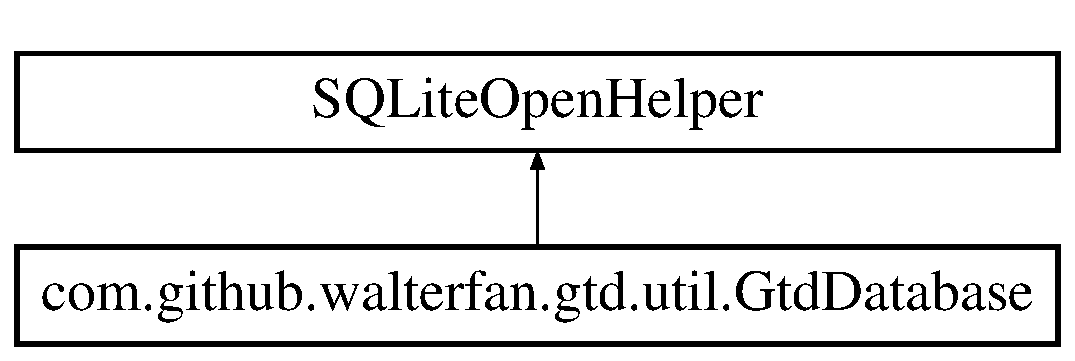
\includegraphics[height=2.000000cm]{classcom_1_1github_1_1walterfan_1_1gtd_1_1util_1_1GtdDatabase}
\end{center}
\end{figure}
\subsection*{Public Member Functions}
\begin{DoxyCompactItemize}
\item 
\hyperlink{classcom_1_1github_1_1walterfan_1_1gtd_1_1util_1_1GtdDatabase_a3e80ee44f75a3b005821f1d078fe605d}{Gtd\-Database} (Context context, String name, Cursor\-Factory factory, int version)
\item 
\hyperlink{classcom_1_1github_1_1walterfan_1_1gtd_1_1util_1_1GtdDatabase_ae7fee67455c42c67ad616ba7c730e241}{Gtd\-Database} (Context context, String name, Cursor\-Factory factory, int version, Database\-Error\-Handler error\-Handler)
\item 
\hypertarget{classcom_1_1github_1_1walterfan_1_1gtd_1_1util_1_1GtdDatabase_a8ab7859d689ca38989723e802667ec1f}{void {\bfseries on\-Create} (S\-Q\-Lite\-Database arg0)}\label{classcom_1_1github_1_1walterfan_1_1gtd_1_1util_1_1GtdDatabase_a8ab7859d689ca38989723e802667ec1f}

\item 
\hypertarget{classcom_1_1github_1_1walterfan_1_1gtd_1_1util_1_1GtdDatabase_a446d976704e723622be388de26f2314c}{void {\bfseries on\-Upgrade} (S\-Q\-Lite\-Database db, int old\-Version, int new\-Version)}\label{classcom_1_1github_1_1walterfan_1_1gtd_1_1util_1_1GtdDatabase_a446d976704e723622be388de26f2314c}

\end{DoxyCompactItemize}


\subsection{Detailed Description}
\begin{DoxyAuthor}{Author}
walter 
\end{DoxyAuthor}


Definition at line 16 of file Gtd\-Database.\-java.



\subsection{Constructor \& Destructor Documentation}
\hypertarget{classcom_1_1github_1_1walterfan_1_1gtd_1_1util_1_1GtdDatabase_a3e80ee44f75a3b005821f1d078fe605d}{\index{com\-::github\-::walterfan\-::gtd\-::util\-::\-Gtd\-Database@{com\-::github\-::walterfan\-::gtd\-::util\-::\-Gtd\-Database}!Gtd\-Database@{Gtd\-Database}}
\index{Gtd\-Database@{Gtd\-Database}!com::github::walterfan::gtd::util::GtdDatabase@{com\-::github\-::walterfan\-::gtd\-::util\-::\-Gtd\-Database}}
\subsubsection[{Gtd\-Database}]{\setlength{\rightskip}{0pt plus 5cm}com.\-github.\-walterfan.\-gtd.\-util.\-Gtd\-Database.\-Gtd\-Database (
\begin{DoxyParamCaption}
\item[{Context}]{context, }
\item[{String}]{name, }
\item[{Cursor\-Factory}]{factory, }
\item[{int}]{version}
\end{DoxyParamCaption}
)\hspace{0.3cm}{\ttfamily [inline]}}}\label{classcom_1_1github_1_1walterfan_1_1gtd_1_1util_1_1GtdDatabase_a3e80ee44f75a3b005821f1d078fe605d}

\begin{DoxyParams}{Parameters}
{\em context} & \\
\hline
{\em name} & \\
\hline
{\em factory} & \\
\hline
{\em version} & \\
\hline
\end{DoxyParams}


Definition at line 33 of file Gtd\-Database.\-java.


\begin{DoxyCode}
33                                                                                          \{
34         super(context, name, factory, version);
35         this.mContext = context;
36     \}
\end{DoxyCode}
\hypertarget{classcom_1_1github_1_1walterfan_1_1gtd_1_1util_1_1GtdDatabase_ae7fee67455c42c67ad616ba7c730e241}{\index{com\-::github\-::walterfan\-::gtd\-::util\-::\-Gtd\-Database@{com\-::github\-::walterfan\-::gtd\-::util\-::\-Gtd\-Database}!Gtd\-Database@{Gtd\-Database}}
\index{Gtd\-Database@{Gtd\-Database}!com::github::walterfan::gtd::util::GtdDatabase@{com\-::github\-::walterfan\-::gtd\-::util\-::\-Gtd\-Database}}
\subsubsection[{Gtd\-Database}]{\setlength{\rightskip}{0pt plus 5cm}com.\-github.\-walterfan.\-gtd.\-util.\-Gtd\-Database.\-Gtd\-Database (
\begin{DoxyParamCaption}
\item[{Context}]{context, }
\item[{String}]{name, }
\item[{Cursor\-Factory}]{factory, }
\item[{int}]{version, }
\item[{Database\-Error\-Handler}]{error\-Handler}
\end{DoxyParamCaption}
)\hspace{0.3cm}{\ttfamily [inline]}}}\label{classcom_1_1github_1_1walterfan_1_1gtd_1_1util_1_1GtdDatabase_ae7fee67455c42c67ad616ba7c730e241}

\begin{DoxyParams}{Parameters}
{\em context} & \\
\hline
{\em name} & \\
\hline
{\em factory} & \\
\hline
{\em version} & \\
\hline
{\em error\-Handler} & \\
\hline
\end{DoxyParams}


Definition at line 45 of file Gtd\-Database.\-java.


\begin{DoxyCode}
46                                                             \{
47         super(context, name, factory, version, errorHandler);
48         this.mContext = context;
49     \}
\end{DoxyCode}


The documentation for this class was generated from the following file\-:\begin{DoxyCompactItemize}
\item 
/cygdrive/d/workspace/java/\-G\-T\-D/src/com/github/walterfan/gtd/util/Gtd\-Database.\-java\end{DoxyCompactItemize}

\hypertarget{interfacecom_1_1github_1_1walterfan_1_1gtd_1_1game_1_1Input}{\section{com.\-github.\-walterfan.\-gtd.\-game.\-Input Interface Reference}
\label{interfacecom_1_1github_1_1walterfan_1_1gtd_1_1game_1_1Input}\index{com.\-github.\-walterfan.\-gtd.\-game.\-Input@{com.\-github.\-walterfan.\-gtd.\-game.\-Input}}
}
\subsection*{Classes}
\begin{DoxyCompactItemize}
\item 
class {\bfseries Key\-Event}
\item 
class {\bfseries Touch\-Event}
\end{DoxyCompactItemize}
\subsection*{Public Member Functions}
\begin{DoxyCompactItemize}
\item 
\hypertarget{interfacecom_1_1github_1_1walterfan_1_1gtd_1_1game_1_1Input_affcfd5492a7e2ec2675d5a75ebbe42bb}{boolean {\bfseries is\-Key\-Pressed} (int key\-Code)}\label{interfacecom_1_1github_1_1walterfan_1_1gtd_1_1game_1_1Input_affcfd5492a7e2ec2675d5a75ebbe42bb}

\item 
\hypertarget{interfacecom_1_1github_1_1walterfan_1_1gtd_1_1game_1_1Input_a48caa76d3b9ffe9658521c490fb0dfaa}{boolean {\bfseries istouch\-Down} (int pointer)}\label{interfacecom_1_1github_1_1walterfan_1_1gtd_1_1game_1_1Input_a48caa76d3b9ffe9658521c490fb0dfaa}

\item 
\hypertarget{interfacecom_1_1github_1_1walterfan_1_1gtd_1_1game_1_1Input_af72fd1fb2872b0337112ebc7b44513b7}{int {\bfseries get\-Touch\-X} (int pointer)}\label{interfacecom_1_1github_1_1walterfan_1_1gtd_1_1game_1_1Input_af72fd1fb2872b0337112ebc7b44513b7}

\item 
\hypertarget{interfacecom_1_1github_1_1walterfan_1_1gtd_1_1game_1_1Input_afc13a5900bdd0770911a28995e455f97}{int {\bfseries get\-Touch\-Y} (int pointer)}\label{interfacecom_1_1github_1_1walterfan_1_1gtd_1_1game_1_1Input_afc13a5900bdd0770911a28995e455f97}

\item 
\hypertarget{interfacecom_1_1github_1_1walterfan_1_1gtd_1_1game_1_1Input_a07e781bf15744e5fbed5440040f18d83}{float {\bfseries get\-Accel\-X} ()}\label{interfacecom_1_1github_1_1walterfan_1_1gtd_1_1game_1_1Input_a07e781bf15744e5fbed5440040f18d83}

\item 
\hypertarget{interfacecom_1_1github_1_1walterfan_1_1gtd_1_1game_1_1Input_a99b3eeefa36e9e8545c68ef52ebcba28}{float {\bfseries get\-Accel\-Y} ()}\label{interfacecom_1_1github_1_1walterfan_1_1gtd_1_1game_1_1Input_a99b3eeefa36e9e8545c68ef52ebcba28}

\item 
\hypertarget{interfacecom_1_1github_1_1walterfan_1_1gtd_1_1game_1_1Input_aff16be8e3467eb45db3869ff6277bd61}{float {\bfseries get\-Accel\-Z} ()}\label{interfacecom_1_1github_1_1walterfan_1_1gtd_1_1game_1_1Input_aff16be8e3467eb45db3869ff6277bd61}

\item 
\hypertarget{interfacecom_1_1github_1_1walterfan_1_1gtd_1_1game_1_1Input_ad9593e512b94ae9d6b109f8f06acaf94}{List$<$ Key\-Event $>$ {\bfseries get\-Key\-Events} ()}\label{interfacecom_1_1github_1_1walterfan_1_1gtd_1_1game_1_1Input_ad9593e512b94ae9d6b109f8f06acaf94}

\item 
\hypertarget{interfacecom_1_1github_1_1walterfan_1_1gtd_1_1game_1_1Input_a669f9b065e37388979ac637b6f1fa63a}{List$<$ Touch\-Event $>$ {\bfseries get\-Touch\-Events} ()}\label{interfacecom_1_1github_1_1walterfan_1_1gtd_1_1game_1_1Input_a669f9b065e37388979ac637b6f1fa63a}

\end{DoxyCompactItemize}


\subsection{Detailed Description}


Definition at line 5 of file Input.\-java.



The documentation for this interface was generated from the following file\-:\begin{DoxyCompactItemize}
\item 
/cygdrive/d/workspace/java/\-G\-T\-D/src/com/github/walterfan/gtd/game/Input.\-java\end{DoxyCompactItemize}

\hypertarget{classwfan_1_1IObserver}{\section{wfan\-:\-:I\-Observer Class Reference}
\label{classwfan_1_1IObserver}\index{wfan\-::\-I\-Observer@{wfan\-::\-I\-Observer}}
}


{\ttfamily \#include $<$Observer.\-h$>$}

\subsection*{Public Member Functions}
\begin{DoxyCompactItemize}
\item 
\hypertarget{classwfan_1_1IObserver_a9c85f7615eb11c5167084a5e8ac9af0b}{virtual void {\bfseries Update} (\hyperlink{classwfan_1_1ISubject}{I\-Subject} $\ast$the\-Changed\-Subject)=0}\label{classwfan_1_1IObserver_a9c85f7615eb11c5167084a5e8ac9af0b}

\end{DoxyCompactItemize}


\subsection{Detailed Description}
Interface \hyperlink{classwfan_1_1IObserver}{I\-Observer} 

Definition at line 23 of file Observer.\-h.



The documentation for this class was generated from the following file\-:\begin{DoxyCompactItemize}
\item 
/cygdrive/d/workspace/java/\-G\-T\-D/jni/util/Observer.\-h\end{DoxyCompactItemize}

\hypertarget{classwfan_1_1ISubject}{\section{wfan\-:\-:I\-Subject Class Reference}
\label{classwfan_1_1ISubject}\index{wfan\-::\-I\-Subject@{wfan\-::\-I\-Subject}}
}


{\ttfamily \#include $<$Observer.\-h$>$}

Inheritance diagram for wfan\-:\-:I\-Subject\-:\begin{figure}[H]
\begin{center}
\leavevmode
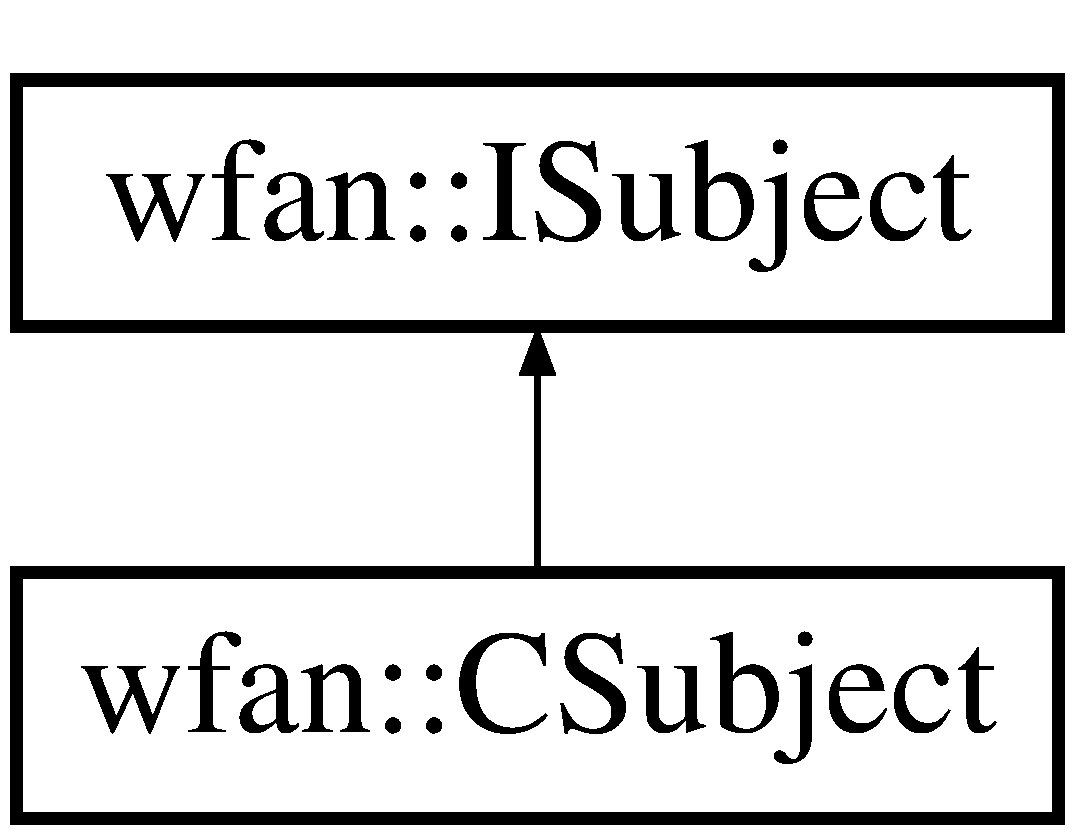
\includegraphics[height=2.000000cm]{classwfan_1_1ISubject}
\end{center}
\end{figure}
\subsection*{Public Member Functions}
\begin{DoxyCompactItemize}
\item 
\hypertarget{classwfan_1_1ISubject_a792e5eccd46e4f45adbb9d2c9b294f16}{virtual void {\bfseries Attach} (\hyperlink{classwfan_1_1IObserver}{I\-Observer} $\ast$p\-Observer)=0}\label{classwfan_1_1ISubject_a792e5eccd46e4f45adbb9d2c9b294f16}

\item 
\hypertarget{classwfan_1_1ISubject_ab7ee968f5fec5937d469c8c5e97ca99b}{virtual void {\bfseries Detach} (\hyperlink{classwfan_1_1IObserver}{I\-Observer} $\ast$p\-Observer)=0}\label{classwfan_1_1ISubject_ab7ee968f5fec5937d469c8c5e97ca99b}

\item 
\hypertarget{classwfan_1_1ISubject_a6e3e9ed80f6e6e838979f7460303c65e}{virtual void {\bfseries Notify} ()=0}\label{classwfan_1_1ISubject_a6e3e9ed80f6e6e838979f7460303c65e}

\end{DoxyCompactItemize}


\subsection{Detailed Description}
Interface \hyperlink{classwfan_1_1ISubject}{I\-Subject} 

Definition at line 36 of file Observer.\-h.



The documentation for this class was generated from the following file\-:\begin{DoxyCompactItemize}
\item 
/cygdrive/d/workspace/java/\-G\-T\-D/jni/util/Observer.\-h\end{DoxyCompactItemize}

\hypertarget{classcom_1_1github_1_1walterfan_1_1gtd_1_1util_1_1JniUtils}{\section{com.\-github.\-walterfan.\-gtd.\-util.\-Jni\-Utils Class Reference}
\label{classcom_1_1github_1_1walterfan_1_1gtd_1_1util_1_1JniUtils}\index{com.\-github.\-walterfan.\-gtd.\-util.\-Jni\-Utils@{com.\-github.\-walterfan.\-gtd.\-util.\-Jni\-Utils}}
}
\subsection*{Static Public Member Functions}
\begin{DoxyCompactItemize}
\item 
\hypertarget{classcom_1_1github_1_1walterfan_1_1gtd_1_1util_1_1JniUtils_a976b186dac97a5ee527dcda412bafa83}{static native void {\bfseries log} (String tag, String msg)}\label{classcom_1_1github_1_1walterfan_1_1gtd_1_1util_1_1JniUtils_a976b186dac97a5ee527dcda412bafa83}

\item 
\hypertarget{classcom_1_1github_1_1walterfan_1_1gtd_1_1util_1_1JniUtils_a92c913d69cdf19bded99261014bf234f}{static native void {\bfseries copy} (Byte\-Buffer dst, float\mbox{[}$\,$\mbox{]} src, int offset, int len)}\label{classcom_1_1github_1_1walterfan_1_1gtd_1_1util_1_1JniUtils_a92c913d69cdf19bded99261014bf234f}

\end{DoxyCompactItemize}


\subsection{Detailed Description}


Definition at line 5 of file Jni\-Utils.\-java.



The documentation for this class was generated from the following file\-:\begin{DoxyCompactItemize}
\item 
/cygdrive/d/workspace/java/\-G\-T\-D/src/com/github/walterfan/gtd/util/Jni\-Utils.\-java\end{DoxyCompactItemize}

\hypertarget{classcom_1_1github_1_1walterfan_1_1gtd_1_1LoginActivity}{\section{com.\-github.\-walterfan.\-gtd.\-Login\-Activity Class Reference}
\label{classcom_1_1github_1_1walterfan_1_1gtd_1_1LoginActivity}\index{com.\-github.\-walterfan.\-gtd.\-Login\-Activity@{com.\-github.\-walterfan.\-gtd.\-Login\-Activity}}
}
Inheritance diagram for com.\-github.\-walterfan.\-gtd.\-Login\-Activity\-:\begin{figure}[H]
\begin{center}
\leavevmode
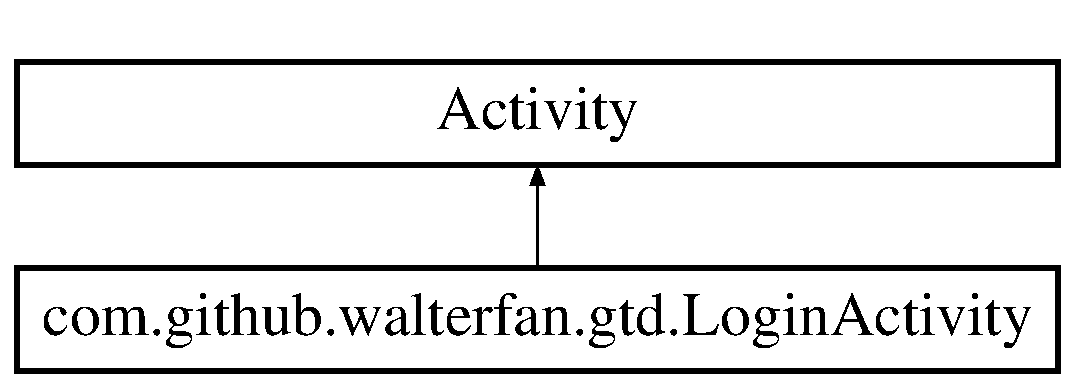
\includegraphics[height=2.000000cm]{classcom_1_1github_1_1walterfan_1_1gtd_1_1LoginActivity}
\end{center}
\end{figure}
\subsection*{Public Member Functions}
\begin{DoxyCompactItemize}
\item 
void \hyperlink{classcom_1_1github_1_1walterfan_1_1gtd_1_1LoginActivity_aa54e52f2826fb79e947a1c15439709ec}{on\-Create} (Bundle saved\-Instance\-State)
\end{DoxyCompactItemize}


\subsection{Detailed Description}


Definition at line 10 of file Login\-Activity.\-java.



\subsection{Member Function Documentation}
\hypertarget{classcom_1_1github_1_1walterfan_1_1gtd_1_1LoginActivity_aa54e52f2826fb79e947a1c15439709ec}{\index{com\-::github\-::walterfan\-::gtd\-::\-Login\-Activity@{com\-::github\-::walterfan\-::gtd\-::\-Login\-Activity}!on\-Create@{on\-Create}}
\index{on\-Create@{on\-Create}!com::github::walterfan::gtd::LoginActivity@{com\-::github\-::walterfan\-::gtd\-::\-Login\-Activity}}
\subsubsection[{on\-Create}]{\setlength{\rightskip}{0pt plus 5cm}void com.\-github.\-walterfan.\-gtd.\-Login\-Activity.\-on\-Create (
\begin{DoxyParamCaption}
\item[{Bundle}]{saved\-Instance\-State}
\end{DoxyParamCaption}
)\hspace{0.3cm}{\ttfamily [inline]}}}\label{classcom_1_1github_1_1walterfan_1_1gtd_1_1LoginActivity_aa54e52f2826fb79e947a1c15439709ec}
Called when the activity is first created. 

Definition at line 21 of file Login\-Activity.\-java.


\begin{DoxyCode}
21                                                     \{
22         super.onCreate(savedInstanceState);
23         
24 
25         setContentView(R.layout.activity\_login);
26         
27         userNameEditText = (EditText)this.findViewById(R.id.userNameEditText);
28         passwordEditText = (EditText)this.findViewById(R.id.passwordEditText);
29         
30         loginButton = (Button)this.findViewById(R.id.loginButton);
31         
32         loginButton.setOnClickListener(\textcolor{keyword}{new} View.OnClickListener() \{
33             
34             \textcolor{keyword}{public} \textcolor{keywordtype}{void} onClick(View v) \{
35                 String userName  = userNameEditText.getText().toString().trim();
36                 String password  = passwordEditText.getText().toString().trim();
37                 
38                 \textcolor{keywordflow}{if}(D) Log.d(TAG, \textcolor{stringliteral}{"Username��"}+userName);
39                 \textcolor{keywordflow}{if}(D) Log.d(TAG, \textcolor{stringliteral}{"Password��"}+password);
40                 
41                 
42                 \textcolor{keywordflow}{if}(\textcolor{stringliteral}{"walter"}.equals(userName) && \textcolor{stringliteral}{"pass"}.equals(password))\{
43                     
44                     Toast.makeText(LoginActivity.this, \textcolor{stringliteral}{"Login successfully!"}, Toast.LENGTH\_SHORT).show();
45                 \}\textcolor{keywordflow}{else}\{
46                     Toast.makeText(LoginActivity.this, \textcolor{stringliteral}{"username or password error!"}, Toast.LENGTH\_SHORT).
      show();
47                 \}
48             \}
49         \});
50         
51     \}
\end{DoxyCode}


The documentation for this class was generated from the following file\-:\begin{DoxyCompactItemize}
\item 
/cygdrive/d/workspace/java/\-G\-T\-D/src/com/github/walterfan/gtd/Login\-Activity.\-java\end{DoxyCompactItemize}

\hypertarget{classcom_1_1github_1_1walterfan_1_1gtd_1_1MainActivity}{\section{com.\-github.\-walterfan.\-gtd.\-Main\-Activity Class Reference}
\label{classcom_1_1github_1_1walterfan_1_1gtd_1_1MainActivity}\index{com.\-github.\-walterfan.\-gtd.\-Main\-Activity@{com.\-github.\-walterfan.\-gtd.\-Main\-Activity}}
}
Inheritance diagram for com.\-github.\-walterfan.\-gtd.\-Main\-Activity\-:\begin{figure}[H]
\begin{center}
\leavevmode
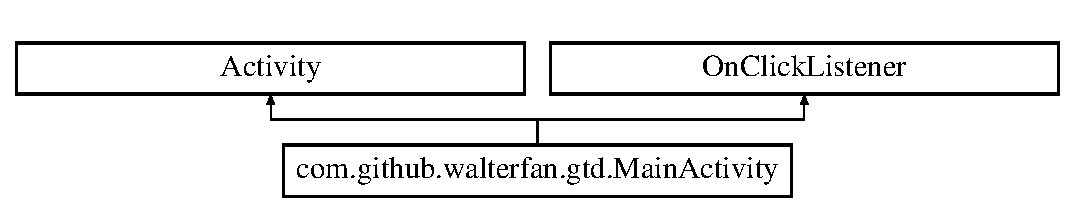
\includegraphics[height=2.000000cm]{classcom_1_1github_1_1walterfan_1_1gtd_1_1MainActivity}
\end{center}
\end{figure}
\subsection*{Public Member Functions}
\begin{DoxyCompactItemize}
\item 
\hypertarget{classcom_1_1github_1_1walterfan_1_1gtd_1_1MainActivity_a815fcc7cc35c40ab378c9619f85f2046}{void {\bfseries add\-Task} (View view)}\label{classcom_1_1github_1_1walterfan_1_1gtd_1_1MainActivity_a815fcc7cc35c40ab378c9619f85f2046}

\item 
\hypertarget{classcom_1_1github_1_1walterfan_1_1gtd_1_1MainActivity_a944bfa4f06700f8b2bad188a86ae0bd3}{boolean {\bfseries on\-Create\-Options\-Menu} (Menu menu)}\label{classcom_1_1github_1_1walterfan_1_1gtd_1_1MainActivity_a944bfa4f06700f8b2bad188a86ae0bd3}

\item 
\hypertarget{classcom_1_1github_1_1walterfan_1_1gtd_1_1MainActivity_aaed11889449cfc6c498e2c7f714bfd50}{boolean {\bfseries on\-Options\-Item\-Selected} (Menu\-Item item)}\label{classcom_1_1github_1_1walterfan_1_1gtd_1_1MainActivity_aaed11889449cfc6c498e2c7f714bfd50}

\item 
\hypertarget{classcom_1_1github_1_1walterfan_1_1gtd_1_1MainActivity_accdfaaa8c057e60730f4d977870c0dbe}{void {\bfseries on\-Click} (View view)}\label{classcom_1_1github_1_1walterfan_1_1gtd_1_1MainActivity_accdfaaa8c057e60730f4d977870c0dbe}

\end{DoxyCompactItemize}
\subsection*{Static Public Attributes}
\begin{DoxyCompactItemize}
\item 
\hypertarget{classcom_1_1github_1_1walterfan_1_1gtd_1_1MainActivity_a7ec58a90574e99cd1690234e4b3ed681}{static final String {\bfseries E\-X\-T\-R\-A\-\_\-\-M\-E\-S\-S\-A\-G\-E} = \char`\"{}com.\-github.\-walterfan.\-gtd.\-M\-E\-S\-S\-A\-G\-E\char`\"{}}\label{classcom_1_1github_1_1walterfan_1_1gtd_1_1MainActivity_a7ec58a90574e99cd1690234e4b3ed681}

\end{DoxyCompactItemize}
\subsection*{Protected Member Functions}
\begin{DoxyCompactItemize}
\item 
\hypertarget{classcom_1_1github_1_1walterfan_1_1gtd_1_1MainActivity_a53383ef32321c58d4489683e6d1bb1d7}{void {\bfseries on\-Create} (Bundle saved\-Instance\-State)}\label{classcom_1_1github_1_1walterfan_1_1gtd_1_1MainActivity_a53383ef32321c58d4489683e6d1bb1d7}

\item 
\hypertarget{classcom_1_1github_1_1walterfan_1_1gtd_1_1MainActivity_a1ded6042012880d7238d75e641341b9e}{void {\bfseries on\-Pause} ()}\label{classcom_1_1github_1_1walterfan_1_1gtd_1_1MainActivity_a1ded6042012880d7238d75e641341b9e}

\item 
\hypertarget{classcom_1_1github_1_1walterfan_1_1gtd_1_1MainActivity_afa16af2fabfbdd75853d550245d4a28d}{void {\bfseries on\-Resume} ()}\label{classcom_1_1github_1_1walterfan_1_1gtd_1_1MainActivity_afa16af2fabfbdd75853d550245d4a28d}

\end{DoxyCompactItemize}


\subsection{Detailed Description}


Definition at line 20 of file Main\-Activity.\-java.



The documentation for this class was generated from the following file\-:\begin{DoxyCompactItemize}
\item 
/cygdrive/d/workspace/java/\-G\-T\-D/src/com/github/walterfan/gtd/Main\-Activity.\-java\end{DoxyCompactItemize}

\hypertarget{classcom_1_1github_1_1walterfan_1_1gtd_1_1test_1_1MediaPlayerTest}{\section{com.\-github.\-walterfan.\-gtd.\-test.\-Media\-Player\-Test Class Reference}
\label{classcom_1_1github_1_1walterfan_1_1gtd_1_1test_1_1MediaPlayerTest}\index{com.\-github.\-walterfan.\-gtd.\-test.\-Media\-Player\-Test@{com.\-github.\-walterfan.\-gtd.\-test.\-Media\-Player\-Test}}
}
Inheritance diagram for com.\-github.\-walterfan.\-gtd.\-test.\-Media\-Player\-Test\-:\begin{figure}[H]
\begin{center}
\leavevmode
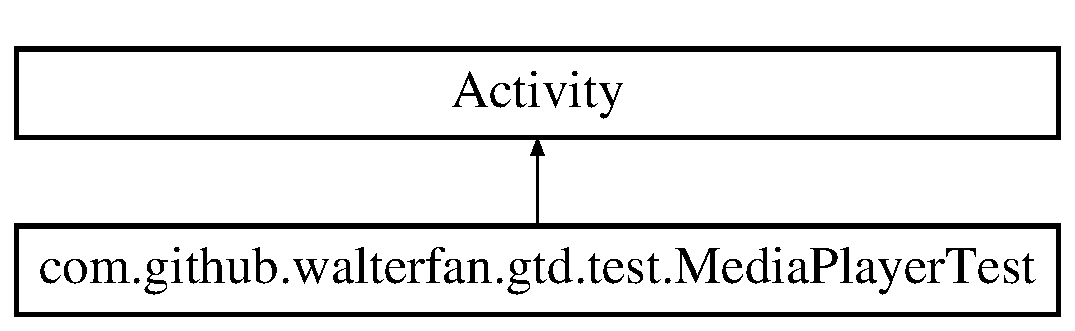
\includegraphics[height=2.000000cm]{classcom_1_1github_1_1walterfan_1_1gtd_1_1test_1_1MediaPlayerTest}
\end{center}
\end{figure}
\subsection*{Public Member Functions}
\begin{DoxyCompactItemize}
\item 
\hypertarget{classcom_1_1github_1_1walterfan_1_1gtd_1_1test_1_1MediaPlayerTest_ad389f3ded89f9ff8e75452b1d9b0bc69}{void {\bfseries on\-Create} (Bundle saved\-Instance\-State)}\label{classcom_1_1github_1_1walterfan_1_1gtd_1_1test_1_1MediaPlayerTest_ad389f3ded89f9ff8e75452b1d9b0bc69}

\end{DoxyCompactItemize}
\subsection*{Protected Member Functions}
\begin{DoxyCompactItemize}
\item 
\hypertarget{classcom_1_1github_1_1walterfan_1_1gtd_1_1test_1_1MediaPlayerTest_a44e33f6f5ff79882cc4f494d06466c0b}{void {\bfseries on\-Resume} ()}\label{classcom_1_1github_1_1walterfan_1_1gtd_1_1test_1_1MediaPlayerTest_a44e33f6f5ff79882cc4f494d06466c0b}

\item 
\hypertarget{classcom_1_1github_1_1walterfan_1_1gtd_1_1test_1_1MediaPlayerTest_a5b02349548c133a1a14b0955158680a9}{void {\bfseries on\-Pause} ()}\label{classcom_1_1github_1_1walterfan_1_1gtd_1_1test_1_1MediaPlayerTest_a5b02349548c133a1a14b0955158680a9}

\end{DoxyCompactItemize}


\subsection{Detailed Description}


Definition at line 14 of file Media\-Player\-Test.\-java.



The documentation for this class was generated from the following file\-:\begin{DoxyCompactItemize}
\item 
/cygdrive/d/workspace/java/\-G\-T\-D/src/com/github/walterfan/gtd/test/Media\-Player\-Test.\-java\end{DoxyCompactItemize}

\hypertarget{interfacecom_1_1github_1_1walterfan_1_1gtd_1_1game_1_1Music}{\section{com.\-github.\-walterfan.\-gtd.\-game.\-Music Interface Reference}
\label{interfacecom_1_1github_1_1walterfan_1_1gtd_1_1game_1_1Music}\index{com.\-github.\-walterfan.\-gtd.\-game.\-Music@{com.\-github.\-walterfan.\-gtd.\-game.\-Music}}
}
\subsection*{Public Member Functions}
\begin{DoxyCompactItemize}
\item 
\hypertarget{interfacecom_1_1github_1_1walterfan_1_1gtd_1_1game_1_1Music_a6332f5ac71cb2adf387bc25f4e480fdf}{void {\bfseries play} ()}\label{interfacecom_1_1github_1_1walterfan_1_1gtd_1_1game_1_1Music_a6332f5ac71cb2adf387bc25f4e480fdf}

\item 
\hypertarget{interfacecom_1_1github_1_1walterfan_1_1gtd_1_1game_1_1Music_aebce2670321a2b1a30df5a827c6a170a}{void {\bfseries stop} ()}\label{interfacecom_1_1github_1_1walterfan_1_1gtd_1_1game_1_1Music_aebce2670321a2b1a30df5a827c6a170a}

\item 
\hypertarget{interfacecom_1_1github_1_1walterfan_1_1gtd_1_1game_1_1Music_abb16e4cc97ecf12fea80869cbe3278f9}{void {\bfseries pause} ()}\label{interfacecom_1_1github_1_1walterfan_1_1gtd_1_1game_1_1Music_abb16e4cc97ecf12fea80869cbe3278f9}

\item 
\hypertarget{interfacecom_1_1github_1_1walterfan_1_1gtd_1_1game_1_1Music_a7963d3a9788212b382cc95f1612fc47d}{void {\bfseries set\-Looping} (boolean looping)}\label{interfacecom_1_1github_1_1walterfan_1_1gtd_1_1game_1_1Music_a7963d3a9788212b382cc95f1612fc47d}

\item 
\hypertarget{interfacecom_1_1github_1_1walterfan_1_1gtd_1_1game_1_1Music_a32f8107ca372cc9aa37245b44074a5d5}{void {\bfseries set\-Volume} (float volume)}\label{interfacecom_1_1github_1_1walterfan_1_1gtd_1_1game_1_1Music_a32f8107ca372cc9aa37245b44074a5d5}

\item 
\hypertarget{interfacecom_1_1github_1_1walterfan_1_1gtd_1_1game_1_1Music_a2927021aa715255e3d5c95042c87506e}{boolean {\bfseries is\-Playing} ()}\label{interfacecom_1_1github_1_1walterfan_1_1gtd_1_1game_1_1Music_a2927021aa715255e3d5c95042c87506e}

\item 
\hypertarget{interfacecom_1_1github_1_1walterfan_1_1gtd_1_1game_1_1Music_a0902b1c673ed8dd92a0bb33140846934}{boolean {\bfseries is\-Stopped} ()}\label{interfacecom_1_1github_1_1walterfan_1_1gtd_1_1game_1_1Music_a0902b1c673ed8dd92a0bb33140846934}

\item 
\hypertarget{interfacecom_1_1github_1_1walterfan_1_1gtd_1_1game_1_1Music_a6bc86c2baea1ec14e96c972983dcb87c}{boolean {\bfseries is\-Looping} ()}\label{interfacecom_1_1github_1_1walterfan_1_1gtd_1_1game_1_1Music_a6bc86c2baea1ec14e96c972983dcb87c}

\item 
\hypertarget{interfacecom_1_1github_1_1walterfan_1_1gtd_1_1game_1_1Music_a54fc265074514024a39823c3038dac87}{void {\bfseries dispose} ()}\label{interfacecom_1_1github_1_1walterfan_1_1gtd_1_1game_1_1Music_a54fc265074514024a39823c3038dac87}

\end{DoxyCompactItemize}


\subsection{Detailed Description}


Definition at line 3 of file Music.\-java.



The documentation for this interface was generated from the following file\-:\begin{DoxyCompactItemize}
\item 
/cygdrive/d/workspace/java/\-G\-T\-D/src/com/github/walterfan/gtd/game/Music.\-java\end{DoxyCompactItemize}

\hypertarget{classcom_1_1github_1_1walterfan_1_1gtd_1_1game_1_1Pixmap}{\section{com.\-github.\-walterfan.\-gtd.\-game.\-Pixmap Class Reference}
\label{classcom_1_1github_1_1walterfan_1_1gtd_1_1game_1_1Pixmap}\index{com.\-github.\-walterfan.\-gtd.\-game.\-Pixmap@{com.\-github.\-walterfan.\-gtd.\-game.\-Pixmap}}
}


\subsection{Detailed Description}


Definition at line 3 of file Pixmap.\-java.



The documentation for this class was generated from the following file\-:\begin{DoxyCompactItemize}
\item 
/cygdrive/d/workspace/java/\-G\-T\-D/src/com/github/walterfan/gtd/game/Pixmap.\-java\end{DoxyCompactItemize}

\hypertarget{enumcom_1_1github_1_1walterfan_1_1gtd_1_1model_1_1Task_1_1Priority}{\section{com.\-github.\-walterfan.\-gtd.\-model.\-Task.\-Priority Enum Reference}
\label{enumcom_1_1github_1_1walterfan_1_1gtd_1_1model_1_1Task_1_1Priority}\index{com.\-github.\-walterfan.\-gtd.\-model.\-Task.\-Priority@{com.\-github.\-walterfan.\-gtd.\-model.\-Task.\-Priority}}
}
\subsection*{Public Attributes}
\begin{DoxyCompactItemize}
\item 
\hypertarget{enumcom_1_1github_1_1walterfan_1_1gtd_1_1model_1_1Task_1_1Priority_a5bd4f3d1449dac07f6e7d84d6c67f291}{{\bfseries I\-M\-P\-O\-R\-T\-A\-N\-T\-\_\-\-U\-R\-G\-E\-N\-T}}\label{enumcom_1_1github_1_1walterfan_1_1gtd_1_1model_1_1Task_1_1Priority_a5bd4f3d1449dac07f6e7d84d6c67f291}

\item 
\hypertarget{enumcom_1_1github_1_1walterfan_1_1gtd_1_1model_1_1Task_1_1Priority_ad5cda79ea9d8aa8ef835107c90644626}{{\bfseries I\-M\-P\-O\-R\-T\-A\-N\-T\-\_\-\-N\-O\-T\-\_\-\-U\-R\-G\-E\-N\-T}}\label{enumcom_1_1github_1_1walterfan_1_1gtd_1_1model_1_1Task_1_1Priority_ad5cda79ea9d8aa8ef835107c90644626}

\item 
\hypertarget{enumcom_1_1github_1_1walterfan_1_1gtd_1_1model_1_1Task_1_1Priority_a010ca9f21f1c8e758252a5a149829077}{{\bfseries N\-O\-T\-\_\-\-I\-M\-P\-O\-R\-T\-A\-N\-T\-\_\-\-U\-R\-G\-E\-N\-T}}\label{enumcom_1_1github_1_1walterfan_1_1gtd_1_1model_1_1Task_1_1Priority_a010ca9f21f1c8e758252a5a149829077}

\item 
\hypertarget{enumcom_1_1github_1_1walterfan_1_1gtd_1_1model_1_1Task_1_1Priority_a0fa45bdfaf8042d4b17bb6e6abfee6ca}{{\bfseries N\-O\-T\-\_\-\-I\-M\-P\-O\-R\-T\-A\-N\-T\-\_\-\-N\-O\-T\-\_\-\-U\-R\-G\-E\-N\-T}}\label{enumcom_1_1github_1_1walterfan_1_1gtd_1_1model_1_1Task_1_1Priority_a0fa45bdfaf8042d4b17bb6e6abfee6ca}

\end{DoxyCompactItemize}


\subsection{Detailed Description}


Definition at line 18 of file Task.\-java.



The documentation for this enum was generated from the following file\-:\begin{DoxyCompactItemize}
\item 
/cygdrive/d/workspace/java/\-G\-T\-D/src/com/github/walterfan/gtd/model/Task.\-java\end{DoxyCompactItemize}

\hypertarget{classcom_1_1github_1_1walterfan_1_1gtd_1_1game_1_1Screen}{\section{com.\-github.\-walterfan.\-gtd.\-game.\-Screen Class Reference}
\label{classcom_1_1github_1_1walterfan_1_1gtd_1_1game_1_1Screen}\index{com.\-github.\-walterfan.\-gtd.\-game.\-Screen@{com.\-github.\-walterfan.\-gtd.\-game.\-Screen}}
}
\subsection*{Public Member Functions}
\begin{DoxyCompactItemize}
\item 
\hypertarget{classcom_1_1github_1_1walterfan_1_1gtd_1_1game_1_1Screen_a06ff9955ff08b7aacbe71bd79f40b52b}{{\bfseries Screen} (\hyperlink{interfacecom_1_1github_1_1walterfan_1_1gtd_1_1game_1_1Game}{Game} game)}\label{classcom_1_1github_1_1walterfan_1_1gtd_1_1game_1_1Screen_a06ff9955ff08b7aacbe71bd79f40b52b}

\item 
\hypertarget{classcom_1_1github_1_1walterfan_1_1gtd_1_1game_1_1Screen_a124881a27f3de26e5082c28e6dfa4a06}{abstract void {\bfseries update} (float delta\-Time)}\label{classcom_1_1github_1_1walterfan_1_1gtd_1_1game_1_1Screen_a124881a27f3de26e5082c28e6dfa4a06}

\item 
\hypertarget{classcom_1_1github_1_1walterfan_1_1gtd_1_1game_1_1Screen_a548c3b3a42d508ef1f6d1cb9d1aa9fbd}{abstract void {\bfseries present} (float delta\-Time)}\label{classcom_1_1github_1_1walterfan_1_1gtd_1_1game_1_1Screen_a548c3b3a42d508ef1f6d1cb9d1aa9fbd}

\item 
\hypertarget{classcom_1_1github_1_1walterfan_1_1gtd_1_1game_1_1Screen_aad708808269151efd008ea646b643ab2}{abstract void {\bfseries pause} ()}\label{classcom_1_1github_1_1walterfan_1_1gtd_1_1game_1_1Screen_aad708808269151efd008ea646b643ab2}

\item 
\hypertarget{classcom_1_1github_1_1walterfan_1_1gtd_1_1game_1_1Screen_ab15c90fb24b27419bf8fff912cf7229f}{abstract void {\bfseries resume} ()}\label{classcom_1_1github_1_1walterfan_1_1gtd_1_1game_1_1Screen_ab15c90fb24b27419bf8fff912cf7229f}

\item 
\hypertarget{classcom_1_1github_1_1walterfan_1_1gtd_1_1game_1_1Screen_aef8d56408a3f67455edd8beb13a60d8b}{abstract void {\bfseries dispose} ()}\label{classcom_1_1github_1_1walterfan_1_1gtd_1_1game_1_1Screen_aef8d56408a3f67455edd8beb13a60d8b}

\end{DoxyCompactItemize}
\subsection*{Protected Attributes}
\begin{DoxyCompactItemize}
\item 
\hypertarget{classcom_1_1github_1_1walterfan_1_1gtd_1_1game_1_1Screen_a46a52c28a126cef2f46cabcfca4ec1e1}{final \hyperlink{interfacecom_1_1github_1_1walterfan_1_1gtd_1_1game_1_1Game}{Game} {\bfseries game}}\label{classcom_1_1github_1_1walterfan_1_1gtd_1_1game_1_1Screen_a46a52c28a126cef2f46cabcfca4ec1e1}

\end{DoxyCompactItemize}


\subsection{Detailed Description}


Definition at line 3 of file Screen.\-java.



The documentation for this class was generated from the following file\-:\begin{DoxyCompactItemize}
\item 
/cygdrive/d/workspace/java/\-G\-T\-D/src/com/github/walterfan/gtd/game/Screen.\-java\end{DoxyCompactItemize}

\hypertarget{classcom_1_1github_1_1walterfan_1_1gtd_1_1test_1_1SensorTest}{\section{com.\-github.\-walterfan.\-gtd.\-test.\-Sensor\-Test Class Reference}
\label{classcom_1_1github_1_1walterfan_1_1gtd_1_1test_1_1SensorTest}\index{com.\-github.\-walterfan.\-gtd.\-test.\-Sensor\-Test@{com.\-github.\-walterfan.\-gtd.\-test.\-Sensor\-Test}}
}
Inheritance diagram for com.\-github.\-walterfan.\-gtd.\-test.\-Sensor\-Test\-:\begin{figure}[H]
\begin{center}
\leavevmode
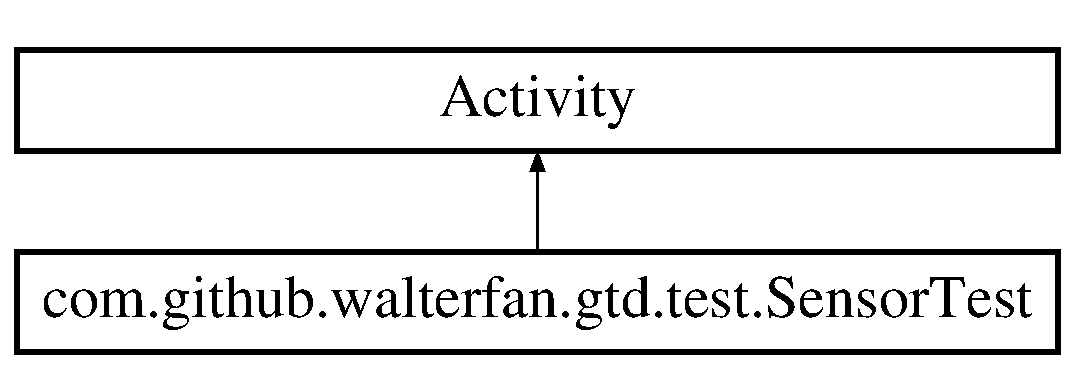
\includegraphics[height=2.000000cm]{classcom_1_1github_1_1walterfan_1_1gtd_1_1test_1_1SensorTest}
\end{center}
\end{figure}
\subsection*{Public Member Functions}
\begin{DoxyCompactItemize}
\item 
\hypertarget{classcom_1_1github_1_1walterfan_1_1gtd_1_1test_1_1SensorTest_a8aa4bd23ffaa67bd31aaae0698688ff4}{boolean {\bfseries on\-Touch\-Event} (Motion\-Event event)}\label{classcom_1_1github_1_1walterfan_1_1gtd_1_1test_1_1SensorTest_a8aa4bd23ffaa67bd31aaae0698688ff4}

\item 
\hypertarget{classcom_1_1github_1_1walterfan_1_1gtd_1_1test_1_1SensorTest_a61c54d54ce42621a35ff9af180e76dd1}{void {\bfseries on\-Resume} ()}\label{classcom_1_1github_1_1walterfan_1_1gtd_1_1test_1_1SensorTest_a61c54d54ce42621a35ff9af180e76dd1}

\item 
\hypertarget{classcom_1_1github_1_1walterfan_1_1gtd_1_1test_1_1SensorTest_aebfa1e75257eabaa49edcf3b19ff2f1c}{void {\bfseries on\-Pause} ()}\label{classcom_1_1github_1_1walterfan_1_1gtd_1_1test_1_1SensorTest_aebfa1e75257eabaa49edcf3b19ff2f1c}

\end{DoxyCompactItemize}
\subsection*{Protected Member Functions}
\begin{DoxyCompactItemize}
\item 
\hypertarget{classcom_1_1github_1_1walterfan_1_1gtd_1_1test_1_1SensorTest_a5accfa4db3a92b45c21abb0b03fdba9e}{void {\bfseries on\-Create} (Bundle saved\-Instance\-State)}\label{classcom_1_1github_1_1walterfan_1_1gtd_1_1test_1_1SensorTest_a5accfa4db3a92b45c21abb0b03fdba9e}

\end{DoxyCompactItemize}


\subsection{Detailed Description}


Definition at line 12 of file Sensor\-Test.\-java.



The documentation for this class was generated from the following file\-:\begin{DoxyCompactItemize}
\item 
/cygdrive/d/workspace/java/\-G\-T\-D/src/com/github/walterfan/gtd/test/Sensor\-Test.\-java\end{DoxyCompactItemize}

\hypertarget{classcom_1_1github_1_1walterfan_1_1gtd_1_1service_1_1DataSyncService_1_1ServiceCountBinder}{\section{com.\-github.\-walterfan.\-gtd.\-service.\-Data\-Sync\-Service.\-Service\-Count\-Binder Class Reference}
\label{classcom_1_1github_1_1walterfan_1_1gtd_1_1service_1_1DataSyncService_1_1ServiceCountBinder}\index{com.\-github.\-walterfan.\-gtd.\-service.\-Data\-Sync\-Service.\-Service\-Count\-Binder@{com.\-github.\-walterfan.\-gtd.\-service.\-Data\-Sync\-Service.\-Service\-Count\-Binder}}
}
Inheritance diagram for com.\-github.\-walterfan.\-gtd.\-service.\-Data\-Sync\-Service.\-Service\-Count\-Binder\-:\begin{figure}[H]
\begin{center}
\leavevmode
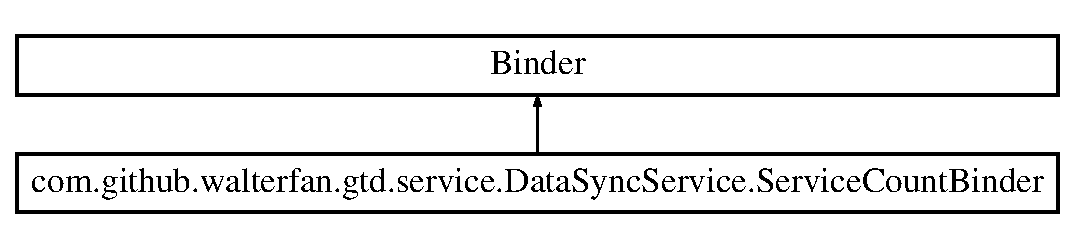
\includegraphics[height=2.000000cm]{classcom_1_1github_1_1walterfan_1_1gtd_1_1service_1_1DataSyncService_1_1ServiceCountBinder}
\end{center}
\end{figure}
\subsection*{Public Member Functions}
\begin{DoxyCompactItemize}
\item 
\hypertarget{classcom_1_1github_1_1walterfan_1_1gtd_1_1service_1_1DataSyncService_1_1ServiceCountBinder_ae6e403b042ad5b1783f8f3c5ad08df2c}{int {\bfseries get\-Service\-Count} ()}\label{classcom_1_1github_1_1walterfan_1_1gtd_1_1service_1_1DataSyncService_1_1ServiceCountBinder_ae6e403b042ad5b1783f8f3c5ad08df2c}

\end{DoxyCompactItemize}


\subsection{Detailed Description}


Definition at line 20 of file Data\-Sync\-Service.\-java.



The documentation for this class was generated from the following file\-:\begin{DoxyCompactItemize}
\item 
/cygdrive/d/workspace/java/\-G\-T\-D/src/com/github/walterfan/gtd/service/Data\-Sync\-Service.\-java\end{DoxyCompactItemize}

\hypertarget{classcom_1_1github_1_1walterfan_1_1gtd_1_1test_1_1ShapeTest}{\section{com.\-github.\-walterfan.\-gtd.\-test.\-Shape\-Test Class Reference}
\label{classcom_1_1github_1_1walterfan_1_1gtd_1_1test_1_1ShapeTest}\index{com.\-github.\-walterfan.\-gtd.\-test.\-Shape\-Test@{com.\-github.\-walterfan.\-gtd.\-test.\-Shape\-Test}}
}
Inheritance diagram for com.\-github.\-walterfan.\-gtd.\-test.\-Shape\-Test\-:\begin{figure}[H]
\begin{center}
\leavevmode
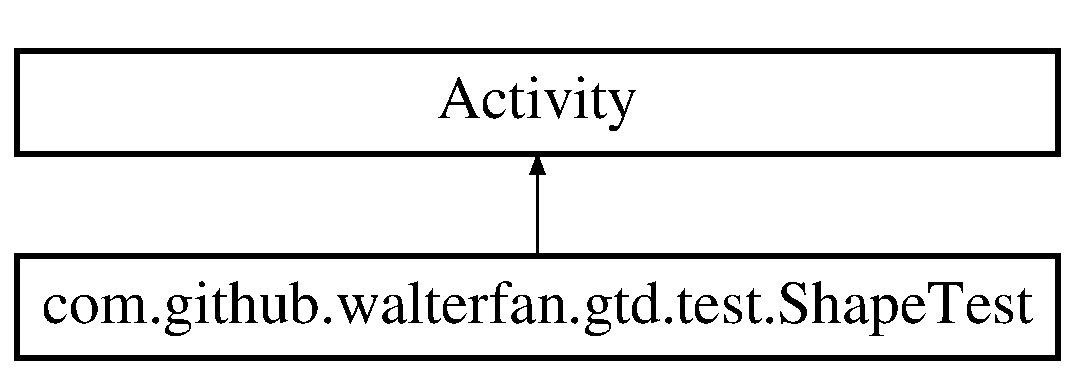
\includegraphics[height=2.000000cm]{classcom_1_1github_1_1walterfan_1_1gtd_1_1test_1_1ShapeTest}
\end{center}
\end{figure}
\subsection*{Classes}
\begin{DoxyCompactItemize}
\item 
class {\bfseries Render\-View}
\end{DoxyCompactItemize}
\subsection*{Protected Member Functions}
\begin{DoxyCompactItemize}
\item 
\hypertarget{classcom_1_1github_1_1walterfan_1_1gtd_1_1test_1_1ShapeTest_ae8f083098155dab718e3f9328e10d6dd}{void {\bfseries on\-Create} (Bundle saved\-Instance\-State)}\label{classcom_1_1github_1_1walterfan_1_1gtd_1_1test_1_1ShapeTest_ae8f083098155dab718e3f9328e10d6dd}

\end{DoxyCompactItemize}


\subsection{Detailed Description}


Definition at line 14 of file Shape\-Test.\-java.



The documentation for this class was generated from the following file\-:\begin{DoxyCompactItemize}
\item 
/cygdrive/d/workspace/java/\-G\-T\-D/src/com/github/walterfan/gtd/test/Shape\-Test.\-java\end{DoxyCompactItemize}

\hypertarget{interfacecom_1_1github_1_1walterfan_1_1gtd_1_1game_1_1Sound}{\section{com.\-github.\-walterfan.\-gtd.\-game.\-Sound Interface Reference}
\label{interfacecom_1_1github_1_1walterfan_1_1gtd_1_1game_1_1Sound}\index{com.\-github.\-walterfan.\-gtd.\-game.\-Sound@{com.\-github.\-walterfan.\-gtd.\-game.\-Sound}}
}
\subsection*{Public Member Functions}
\begin{DoxyCompactItemize}
\item 
\hypertarget{interfacecom_1_1github_1_1walterfan_1_1gtd_1_1game_1_1Sound_ae49912767e70da1f99a0b72243accabf}{void {\bfseries play} (float bolume)}\label{interfacecom_1_1github_1_1walterfan_1_1gtd_1_1game_1_1Sound_ae49912767e70da1f99a0b72243accabf}

\item 
\hypertarget{interfacecom_1_1github_1_1walterfan_1_1gtd_1_1game_1_1Sound_a723e3eec2b0e35c7cfec2473be94a956}{void {\bfseries dispose} ()}\label{interfacecom_1_1github_1_1walterfan_1_1gtd_1_1game_1_1Sound_a723e3eec2b0e35c7cfec2473be94a956}

\end{DoxyCompactItemize}


\subsection{Detailed Description}


Definition at line 3 of file Sound.\-java.



The documentation for this interface was generated from the following file\-:\begin{DoxyCompactItemize}
\item 
/cygdrive/d/workspace/java/\-G\-T\-D/src/com/github/walterfan/gtd/game/Sound.\-java\end{DoxyCompactItemize}

\hypertarget{classcom_1_1github_1_1walterfan_1_1gtd_1_1test_1_1SoundPoolTest}{\section{com.\-github.\-walterfan.\-gtd.\-test.\-Sound\-Pool\-Test Class Reference}
\label{classcom_1_1github_1_1walterfan_1_1gtd_1_1test_1_1SoundPoolTest}\index{com.\-github.\-walterfan.\-gtd.\-test.\-Sound\-Pool\-Test@{com.\-github.\-walterfan.\-gtd.\-test.\-Sound\-Pool\-Test}}
}
Inheritance diagram for com.\-github.\-walterfan.\-gtd.\-test.\-Sound\-Pool\-Test\-:\begin{figure}[H]
\begin{center}
\leavevmode
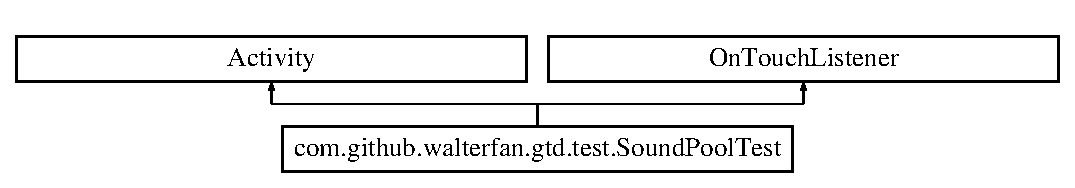
\includegraphics[height=2.000000cm]{classcom_1_1github_1_1walterfan_1_1gtd_1_1test_1_1SoundPoolTest}
\end{center}
\end{figure}
\subsection*{Public Member Functions}
\begin{DoxyCompactItemize}
\item 
\hypertarget{classcom_1_1github_1_1walterfan_1_1gtd_1_1test_1_1SoundPoolTest_ae1ca230363b4b7dbd96904a4fb1be056}{boolean {\bfseries on\-Touch} (View view, Motion\-Event event)}\label{classcom_1_1github_1_1walterfan_1_1gtd_1_1test_1_1SoundPoolTest_ae1ca230363b4b7dbd96904a4fb1be056}

\item 
\hypertarget{classcom_1_1github_1_1walterfan_1_1gtd_1_1test_1_1SoundPoolTest_a507ad52810297750faab436e9d46ca5e}{void {\bfseries on\-Create} (Bundle saved\-Instance\-State)}\label{classcom_1_1github_1_1walterfan_1_1gtd_1_1test_1_1SoundPoolTest_a507ad52810297750faab436e9d46ca5e}

\end{DoxyCompactItemize}


\subsection{Detailed Description}


Definition at line 17 of file Sound\-Pool\-Test.\-java.



The documentation for this class was generated from the following file\-:\begin{DoxyCompactItemize}
\item 
/cygdrive/d/workspace/java/\-G\-T\-D/src/com/github/walterfan/gtd/test/Sound\-Pool\-Test.\-java\end{DoxyCompactItemize}

\hypertarget{classcom_1_1github_1_1walterfan_1_1gtd_1_1model_1_1Task}{\section{com.\-github.\-walterfan.\-gtd.\-model.\-Task Class Reference}
\label{classcom_1_1github_1_1walterfan_1_1gtd_1_1model_1_1Task}\index{com.\-github.\-walterfan.\-gtd.\-model.\-Task@{com.\-github.\-walterfan.\-gtd.\-model.\-Task}}
}
Inheritance diagram for com.\-github.\-walterfan.\-gtd.\-model.\-Task\-:\begin{figure}[H]
\begin{center}
\leavevmode
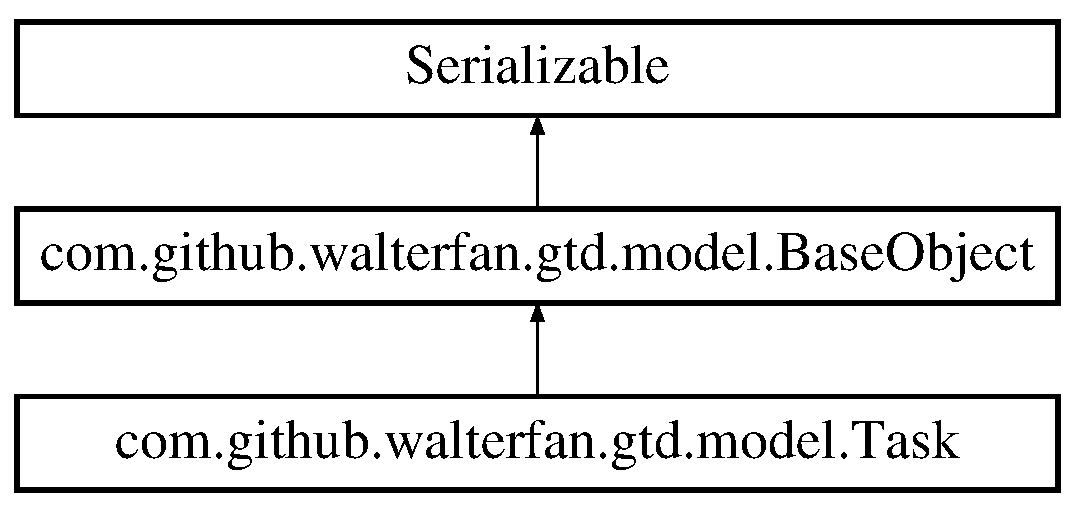
\includegraphics[height=3.000000cm]{classcom_1_1github_1_1walterfan_1_1gtd_1_1model_1_1Task}
\end{center}
\end{figure}
\subsection*{Classes}
\begin{DoxyCompactItemize}
\item 
enum \hyperlink{enumcom_1_1github_1_1walterfan_1_1gtd_1_1model_1_1Task_1_1Priority}{Priority}
\end{DoxyCompactItemize}
\subsection*{Public Member Functions}
\begin{DoxyCompactItemize}
\item 
\hypertarget{classcom_1_1github_1_1walterfan_1_1gtd_1_1model_1_1Task_a4b6cab9d8acb169572537ceaa0d869b7}{{\bfseries Task} (\hyperlink{classcom_1_1github_1_1walterfan_1_1gtd_1_1model_1_1Task}{Task} a\-Task)}\label{classcom_1_1github_1_1walterfan_1_1gtd_1_1model_1_1Task_a4b6cab9d8acb169572537ceaa0d869b7}

\item 
\hypertarget{classcom_1_1github_1_1walterfan_1_1gtd_1_1model_1_1Task_a269f4b8dd7d6a51d8a00dfac3e026d52}{int {\bfseries get\-Context\-I\-D} ()}\label{classcom_1_1github_1_1walterfan_1_1gtd_1_1model_1_1Task_a269f4b8dd7d6a51d8a00dfac3e026d52}

\item 
\hypertarget{classcom_1_1github_1_1walterfan_1_1gtd_1_1model_1_1Task_a829f8a641ab7541fe844e9c14210c188}{void {\bfseries set\-Context\-I\-D} (int context\-I\-D)}\label{classcom_1_1github_1_1walterfan_1_1gtd_1_1model_1_1Task_a829f8a641ab7541fe844e9c14210c188}

\item 
\hypertarget{classcom_1_1github_1_1walterfan_1_1gtd_1_1model_1_1Task_a88c097c5762c018bcbb746ea6f63d23c}{int {\bfseries get\-Task\-Type} ()}\label{classcom_1_1github_1_1walterfan_1_1gtd_1_1model_1_1Task_a88c097c5762c018bcbb746ea6f63d23c}

\item 
\hypertarget{classcom_1_1github_1_1walterfan_1_1gtd_1_1model_1_1Task_a2ed272f392a4e1f8aaecd8bb14305da2}{void {\bfseries set\-Task\-Type} (int task\-Type)}\label{classcom_1_1github_1_1walterfan_1_1gtd_1_1model_1_1Task_a2ed272f392a4e1f8aaecd8bb14305da2}

\item 
\hypertarget{classcom_1_1github_1_1walterfan_1_1gtd_1_1model_1_1Task_a9a841af59f68d6aa59f9dadce48d40cf}{int {\bfseries get\-Energy} ()}\label{classcom_1_1github_1_1walterfan_1_1gtd_1_1model_1_1Task_a9a841af59f68d6aa59f9dadce48d40cf}

\item 
\hypertarget{classcom_1_1github_1_1walterfan_1_1gtd_1_1model_1_1Task_aba16c99450ab1b0d40e1ffa515d89f50}{void {\bfseries set\-Energy} (int energy)}\label{classcom_1_1github_1_1walterfan_1_1gtd_1_1model_1_1Task_aba16c99450ab1b0d40e1ffa515d89f50}

\item 
\hypertarget{classcom_1_1github_1_1walterfan_1_1gtd_1_1model_1_1Task_acdd3b40ff831557c5bd79e87a60694ec}{int {\bfseries get\-Task\-I\-D} ()}\label{classcom_1_1github_1_1walterfan_1_1gtd_1_1model_1_1Task_acdd3b40ff831557c5bd79e87a60694ec}

\item 
\hypertarget{classcom_1_1github_1_1walterfan_1_1gtd_1_1model_1_1Task_aff1a1e754dac0cb5a60506c3895a9238}{void {\bfseries set\-Task\-I\-D} (int task\-I\-D)}\label{classcom_1_1github_1_1walterfan_1_1gtd_1_1model_1_1Task_aff1a1e754dac0cb5a60506c3895a9238}

\item 
\hypertarget{classcom_1_1github_1_1walterfan_1_1gtd_1_1model_1_1Task_acc51d6f12a414f148fbc19a0dc4ab265}{String {\bfseries get\-Task\-Name} ()}\label{classcom_1_1github_1_1walterfan_1_1gtd_1_1model_1_1Task_acc51d6f12a414f148fbc19a0dc4ab265}

\item 
\hypertarget{classcom_1_1github_1_1walterfan_1_1gtd_1_1model_1_1Task_a8107bb1c739d04307cae40643c545cb1}{void {\bfseries set\-Task\-Name} (String task\-Name)}\label{classcom_1_1github_1_1walterfan_1_1gtd_1_1model_1_1Task_a8107bb1c739d04307cae40643c545cb1}

\item 
\hypertarget{classcom_1_1github_1_1walterfan_1_1gtd_1_1model_1_1Task_af9328edbf78657f35345bafb4fad503c}{int {\bfseries get\-Priority} ()}\label{classcom_1_1github_1_1walterfan_1_1gtd_1_1model_1_1Task_af9328edbf78657f35345bafb4fad503c}

\item 
\hypertarget{classcom_1_1github_1_1walterfan_1_1gtd_1_1model_1_1Task_a581457c0f5f18355b9e71c2726b24a12}{void {\bfseries set\-Priority} (int priority)}\label{classcom_1_1github_1_1walterfan_1_1gtd_1_1model_1_1Task_a581457c0f5f18355b9e71c2726b24a12}

\item 
\hypertarget{classcom_1_1github_1_1walterfan_1_1gtd_1_1model_1_1Task_a0d3da594853ebed1edc9c5cbe62c3630}{Timestamp {\bfseries get\-Deadline} ()}\label{classcom_1_1github_1_1walterfan_1_1gtd_1_1model_1_1Task_a0d3da594853ebed1edc9c5cbe62c3630}

\item 
\hypertarget{classcom_1_1github_1_1walterfan_1_1gtd_1_1model_1_1Task_a015b223995adffbf0beffc420091b697}{void {\bfseries set\-Deadline} (Timestamp deadline)}\label{classcom_1_1github_1_1walterfan_1_1gtd_1_1model_1_1Task_a015b223995adffbf0beffc420091b697}

\item 
\hypertarget{classcom_1_1github_1_1walterfan_1_1gtd_1_1model_1_1Task_addc38f1a93a762601f1f059ff4a236a0}{int {\bfseries get\-Duration} ()}\label{classcom_1_1github_1_1walterfan_1_1gtd_1_1model_1_1Task_addc38f1a93a762601f1f059ff4a236a0}

\item 
\hypertarget{classcom_1_1github_1_1walterfan_1_1gtd_1_1model_1_1Task_a9e7cae68e10d30b4185d479078297c50}{void {\bfseries set\-Duration} (int duration)}\label{classcom_1_1github_1_1walterfan_1_1gtd_1_1model_1_1Task_a9e7cae68e10d30b4185d479078297c50}

\item 
\hypertarget{classcom_1_1github_1_1walterfan_1_1gtd_1_1model_1_1Task_aa2cfd3718dcb5177551545deb67be23f}{String {\bfseries get\-Description} ()}\label{classcom_1_1github_1_1walterfan_1_1gtd_1_1model_1_1Task_aa2cfd3718dcb5177551545deb67be23f}

\item 
\hypertarget{classcom_1_1github_1_1walterfan_1_1gtd_1_1model_1_1Task_a79056917cb772d7d3a20cfa70fb2cf07}{void {\bfseries set\-Description} (String description)}\label{classcom_1_1github_1_1walterfan_1_1gtd_1_1model_1_1Task_a79056917cb772d7d3a20cfa70fb2cf07}

\item 
Timestamp \hyperlink{classcom_1_1github_1_1walterfan_1_1gtd_1_1model_1_1Task_a54fe391f305709f61aeace1d597d4383}{get\-Create\-Time} ()
\item 
void \hyperlink{classcom_1_1github_1_1walterfan_1_1gtd_1_1model_1_1Task_a2b316bb20e25c3ec065fc9e4f7059c23}{set\-Create\-Time} (Timestamp create\-Time)
\item 
Timestamp \hyperlink{classcom_1_1github_1_1walterfan_1_1gtd_1_1model_1_1Task_a9a3fb9c8f8b044f8fdc155a7c437995f}{get\-Begin\-Time} ()
\item 
void \hyperlink{classcom_1_1github_1_1walterfan_1_1gtd_1_1model_1_1Task_a1776b1841bbef0b6b88b714704fe89e3}{set\-Begin\-Time} (Timestamp begin\-Time)
\item 
Timestamp \hyperlink{classcom_1_1github_1_1walterfan_1_1gtd_1_1model_1_1Task_ac9a8851fb16d0ceeca479095a0bd984f}{get\-End\-Time} ()
\item 
void \hyperlink{classcom_1_1github_1_1walterfan_1_1gtd_1_1model_1_1Task_a754690b4dca6d8e1ad5e04dc83cad754}{set\-End\-Time} (Timestamp end\-Time)
\item 
int \hyperlink{classcom_1_1github_1_1walterfan_1_1gtd_1_1model_1_1Task_aac748862b11c8ec34537dd375fbed121}{get\-User\-I\-D} ()
\item 
void \hyperlink{classcom_1_1github_1_1walterfan_1_1gtd_1_1model_1_1Task_a8e01883c4b75badddb9473d43e998552}{set\-User\-I\-D} (int user\-I\-D)
\item 
int \hyperlink{classcom_1_1github_1_1walterfan_1_1gtd_1_1model_1_1Task_a1d15293987c115254a1d5711fe681e39}{get\-Category\-I\-D} ()
\item 
void \hyperlink{classcom_1_1github_1_1walterfan_1_1gtd_1_1model_1_1Task_a0f2ccbf29bdeda41d8907567940cfec0}{set\-Category\-I\-D} (int category\-I\-D)
\item 
int \hyperlink{classcom_1_1github_1_1walterfan_1_1gtd_1_1model_1_1Task_a6334be40340ec191f334c9557fa134fc}{get\-Repeat\-I\-D} ()
\item 
void \hyperlink{classcom_1_1github_1_1walterfan_1_1gtd_1_1model_1_1Task_a7bfadd819620e6bfe35023f23e2da14b}{set\-Repeat\-I\-D} (int repeat\-I\-D)
\item 
int \hyperlink{classcom_1_1github_1_1walterfan_1_1gtd_1_1model_1_1Task_a6122723e306af4bdd9cf944e2a03553c}{get\-Remind\-I\-D} ()
\item 
void \hyperlink{classcom_1_1github_1_1walterfan_1_1gtd_1_1model_1_1Task_a8227d6ef7922ff0d82cbca5936d355d6}{set\-Remind\-I\-D} (int remind\-I\-D)
\end{DoxyCompactItemize}
\subsection*{Static Public Member Functions}
\begin{DoxyCompactItemize}
\item 
\hypertarget{classcom_1_1github_1_1walterfan_1_1gtd_1_1model_1_1Task_aea09089803ff3d52da80906309b8f058}{static Map$<$ Integer, String $>$ {\bfseries get\-Task\-Types} ()}\label{classcom_1_1github_1_1walterfan_1_1gtd_1_1model_1_1Task_aea09089803ff3d52da80906309b8f058}

\end{DoxyCompactItemize}
\subsection*{Static Public Attributes}
\begin{DoxyCompactItemize}
\item 
\hypertarget{classcom_1_1github_1_1walterfan_1_1gtd_1_1model_1_1Task_a27ceac7a0950538c2c40e367dbcb9019}{static final int {\bfseries T\-A\-S\-K\-T\-Y\-P\-E\-\_\-\-U\-N\-D\-E\-F\-I\-N\-E\-D} = 0}\label{classcom_1_1github_1_1walterfan_1_1gtd_1_1model_1_1Task_a27ceac7a0950538c2c40e367dbcb9019}

\item 
\hypertarget{classcom_1_1github_1_1walterfan_1_1gtd_1_1model_1_1Task_a94dd1b8e23c2e9997a8c1ac39d95073d}{static final int {\bfseries T\-A\-S\-K\-T\-Y\-P\-E\-\_\-\-N\-E\-X\-T\-A\-C\-T\-I\-O\-N} = 1}\label{classcom_1_1github_1_1walterfan_1_1gtd_1_1model_1_1Task_a94dd1b8e23c2e9997a8c1ac39d95073d}

\item 
\hypertarget{classcom_1_1github_1_1walterfan_1_1gtd_1_1model_1_1Task_a868e1a5eb17d14c5ad02a7a5f52c8fe6}{static final int {\bfseries T\-A\-S\-K\-T\-Y\-P\-E\-\_\-\-O\-N\-S\-C\-H\-E\-D\-U\-L\-E} = 2}\label{classcom_1_1github_1_1walterfan_1_1gtd_1_1model_1_1Task_a868e1a5eb17d14c5ad02a7a5f52c8fe6}

\item 
\hypertarget{classcom_1_1github_1_1walterfan_1_1gtd_1_1model_1_1Task_a985cdc8b9d1c834cbba93f76aea6184b}{static final int {\bfseries T\-A\-S\-K\-T\-Y\-P\-E\-\_\-\-W\-A\-I\-T\-O\-T\-H\-E\-R\-S} = 3}\label{classcom_1_1github_1_1walterfan_1_1gtd_1_1model_1_1Task_a985cdc8b9d1c834cbba93f76aea6184b}

\end{DoxyCompactItemize}
\subsection*{Protected Attributes}
\begin{DoxyCompactItemize}
\item 
\hypertarget{classcom_1_1github_1_1walterfan_1_1gtd_1_1model_1_1Task_a953bf99b63360fae63af565e554fed54}{int {\bfseries repeat\-I\-D} = 0}\label{classcom_1_1github_1_1walterfan_1_1gtd_1_1model_1_1Task_a953bf99b63360fae63af565e554fed54}

\end{DoxyCompactItemize}
\subsection*{Additional Inherited Members}


\subsection{Detailed Description}


Definition at line 7 of file Task.\-java.



\subsection{Member Function Documentation}
\hypertarget{classcom_1_1github_1_1walterfan_1_1gtd_1_1model_1_1Task_a9a3fb9c8f8b044f8fdc155a7c437995f}{\index{com\-::github\-::walterfan\-::gtd\-::model\-::\-Task@{com\-::github\-::walterfan\-::gtd\-::model\-::\-Task}!get\-Begin\-Time@{get\-Begin\-Time}}
\index{get\-Begin\-Time@{get\-Begin\-Time}!com::github::walterfan::gtd::model::Task@{com\-::github\-::walterfan\-::gtd\-::model\-::\-Task}}
\subsubsection[{get\-Begin\-Time}]{\setlength{\rightskip}{0pt plus 5cm}Timestamp com.\-github.\-walterfan.\-gtd.\-model.\-Task.\-get\-Begin\-Time (
\begin{DoxyParamCaption}
{}
\end{DoxyParamCaption}
)\hspace{0.3cm}{\ttfamily [inline]}}}\label{classcom_1_1github_1_1walterfan_1_1gtd_1_1model_1_1Task_a9a3fb9c8f8b044f8fdc155a7c437995f}
\begin{DoxyReturn}{Returns}
the begin\-Time 
\end{DoxyReturn}


Definition at line 163 of file Task.\-java.


\begin{DoxyCode}
163                                     \{
164         \textcolor{keywordflow}{return} beginTime;
165     \}
\end{DoxyCode}
\hypertarget{classcom_1_1github_1_1walterfan_1_1gtd_1_1model_1_1Task_a1d15293987c115254a1d5711fe681e39}{\index{com\-::github\-::walterfan\-::gtd\-::model\-::\-Task@{com\-::github\-::walterfan\-::gtd\-::model\-::\-Task}!get\-Category\-I\-D@{get\-Category\-I\-D}}
\index{get\-Category\-I\-D@{get\-Category\-I\-D}!com::github::walterfan::gtd::model::Task@{com\-::github\-::walterfan\-::gtd\-::model\-::\-Task}}
\subsubsection[{get\-Category\-I\-D}]{\setlength{\rightskip}{0pt plus 5cm}int com.\-github.\-walterfan.\-gtd.\-model.\-Task.\-get\-Category\-I\-D (
\begin{DoxyParamCaption}
{}
\end{DoxyParamCaption}
)\hspace{0.3cm}{\ttfamily [inline]}}}\label{classcom_1_1github_1_1walterfan_1_1gtd_1_1model_1_1Task_a1d15293987c115254a1d5711fe681e39}
\begin{DoxyReturn}{Returns}
the category\-I\-D 
\end{DoxyReturn}


Definition at line 206 of file Task.\-java.


\begin{DoxyCode}
206                                \{
207         \textcolor{keywordflow}{return} categoryID;
208     \}
\end{DoxyCode}
\hypertarget{classcom_1_1github_1_1walterfan_1_1gtd_1_1model_1_1Task_a54fe391f305709f61aeace1d597d4383}{\index{com\-::github\-::walterfan\-::gtd\-::model\-::\-Task@{com\-::github\-::walterfan\-::gtd\-::model\-::\-Task}!get\-Create\-Time@{get\-Create\-Time}}
\index{get\-Create\-Time@{get\-Create\-Time}!com::github::walterfan::gtd::model::Task@{com\-::github\-::walterfan\-::gtd\-::model\-::\-Task}}
\subsubsection[{get\-Create\-Time}]{\setlength{\rightskip}{0pt plus 5cm}Timestamp com.\-github.\-walterfan.\-gtd.\-model.\-Task.\-get\-Create\-Time (
\begin{DoxyParamCaption}
{}
\end{DoxyParamCaption}
)\hspace{0.3cm}{\ttfamily [inline]}}}\label{classcom_1_1github_1_1walterfan_1_1gtd_1_1model_1_1Task_a54fe391f305709f61aeace1d597d4383}
\begin{DoxyReturn}{Returns}
the create\-Time 
\end{DoxyReturn}


Definition at line 149 of file Task.\-java.


\begin{DoxyCode}
149                                      \{
150         \textcolor{keywordflow}{return} createTime;
151     \}
\end{DoxyCode}
\hypertarget{classcom_1_1github_1_1walterfan_1_1gtd_1_1model_1_1Task_ac9a8851fb16d0ceeca479095a0bd984f}{\index{com\-::github\-::walterfan\-::gtd\-::model\-::\-Task@{com\-::github\-::walterfan\-::gtd\-::model\-::\-Task}!get\-End\-Time@{get\-End\-Time}}
\index{get\-End\-Time@{get\-End\-Time}!com::github::walterfan::gtd::model::Task@{com\-::github\-::walterfan\-::gtd\-::model\-::\-Task}}
\subsubsection[{get\-End\-Time}]{\setlength{\rightskip}{0pt plus 5cm}Timestamp com.\-github.\-walterfan.\-gtd.\-model.\-Task.\-get\-End\-Time (
\begin{DoxyParamCaption}
{}
\end{DoxyParamCaption}
)\hspace{0.3cm}{\ttfamily [inline]}}}\label{classcom_1_1github_1_1walterfan_1_1gtd_1_1model_1_1Task_ac9a8851fb16d0ceeca479095a0bd984f}
\begin{DoxyReturn}{Returns}
the end\-Time 
\end{DoxyReturn}


Definition at line 177 of file Task.\-java.


\begin{DoxyCode}
177                                   \{
178         \textcolor{keywordflow}{return} endTime;
179     \}
\end{DoxyCode}
\hypertarget{classcom_1_1github_1_1walterfan_1_1gtd_1_1model_1_1Task_a6122723e306af4bdd9cf944e2a03553c}{\index{com\-::github\-::walterfan\-::gtd\-::model\-::\-Task@{com\-::github\-::walterfan\-::gtd\-::model\-::\-Task}!get\-Remind\-I\-D@{get\-Remind\-I\-D}}
\index{get\-Remind\-I\-D@{get\-Remind\-I\-D}!com::github::walterfan::gtd::model::Task@{com\-::github\-::walterfan\-::gtd\-::model\-::\-Task}}
\subsubsection[{get\-Remind\-I\-D}]{\setlength{\rightskip}{0pt plus 5cm}int com.\-github.\-walterfan.\-gtd.\-model.\-Task.\-get\-Remind\-I\-D (
\begin{DoxyParamCaption}
{}
\end{DoxyParamCaption}
)\hspace{0.3cm}{\ttfamily [inline]}}}\label{classcom_1_1github_1_1walterfan_1_1gtd_1_1model_1_1Task_a6122723e306af4bdd9cf944e2a03553c}
\begin{DoxyReturn}{Returns}
the remind\-I\-D 
\end{DoxyReturn}


Definition at line 246 of file Task.\-java.


\begin{DoxyCode}
246                              \{
247         \textcolor{keywordflow}{return} remindID;
248     \}
\end{DoxyCode}
\hypertarget{classcom_1_1github_1_1walterfan_1_1gtd_1_1model_1_1Task_a6334be40340ec191f334c9557fa134fc}{\index{com\-::github\-::walterfan\-::gtd\-::model\-::\-Task@{com\-::github\-::walterfan\-::gtd\-::model\-::\-Task}!get\-Repeat\-I\-D@{get\-Repeat\-I\-D}}
\index{get\-Repeat\-I\-D@{get\-Repeat\-I\-D}!com::github::walterfan::gtd::model::Task@{com\-::github\-::walterfan\-::gtd\-::model\-::\-Task}}
\subsubsection[{get\-Repeat\-I\-D}]{\setlength{\rightskip}{0pt plus 5cm}int com.\-github.\-walterfan.\-gtd.\-model.\-Task.\-get\-Repeat\-I\-D (
\begin{DoxyParamCaption}
{}
\end{DoxyParamCaption}
)\hspace{0.3cm}{\ttfamily [inline]}}}\label{classcom_1_1github_1_1walterfan_1_1gtd_1_1model_1_1Task_a6334be40340ec191f334c9557fa134fc}
\begin{DoxyReturn}{Returns}
the repeat\-I\-D 
\end{DoxyReturn}


Definition at line 230 of file Task.\-java.


\begin{DoxyCode}
230                              \{
231         \textcolor{keywordflow}{return} repeatID;
232     \}
\end{DoxyCode}
\hypertarget{classcom_1_1github_1_1walterfan_1_1gtd_1_1model_1_1Task_aac748862b11c8ec34537dd375fbed121}{\index{com\-::github\-::walterfan\-::gtd\-::model\-::\-Task@{com\-::github\-::walterfan\-::gtd\-::model\-::\-Task}!get\-User\-I\-D@{get\-User\-I\-D}}
\index{get\-User\-I\-D@{get\-User\-I\-D}!com::github::walterfan::gtd::model::Task@{com\-::github\-::walterfan\-::gtd\-::model\-::\-Task}}
\subsubsection[{get\-User\-I\-D}]{\setlength{\rightskip}{0pt plus 5cm}int com.\-github.\-walterfan.\-gtd.\-model.\-Task.\-get\-User\-I\-D (
\begin{DoxyParamCaption}
{}
\end{DoxyParamCaption}
)\hspace{0.3cm}{\ttfamily [inline]}}}\label{classcom_1_1github_1_1walterfan_1_1gtd_1_1model_1_1Task_aac748862b11c8ec34537dd375fbed121}
\begin{DoxyReturn}{Returns}
the user\-I\-D 
\end{DoxyReturn}


Definition at line 192 of file Task.\-java.


\begin{DoxyCode}
192                            \{
193         \textcolor{keywordflow}{return} userID;
194     \}
\end{DoxyCode}
\hypertarget{classcom_1_1github_1_1walterfan_1_1gtd_1_1model_1_1Task_a1776b1841bbef0b6b88b714704fe89e3}{\index{com\-::github\-::walterfan\-::gtd\-::model\-::\-Task@{com\-::github\-::walterfan\-::gtd\-::model\-::\-Task}!set\-Begin\-Time@{set\-Begin\-Time}}
\index{set\-Begin\-Time@{set\-Begin\-Time}!com::github::walterfan::gtd::model::Task@{com\-::github\-::walterfan\-::gtd\-::model\-::\-Task}}
\subsubsection[{set\-Begin\-Time}]{\setlength{\rightskip}{0pt plus 5cm}void com.\-github.\-walterfan.\-gtd.\-model.\-Task.\-set\-Begin\-Time (
\begin{DoxyParamCaption}
\item[{Timestamp}]{begin\-Time}
\end{DoxyParamCaption}
)\hspace{0.3cm}{\ttfamily [inline]}}}\label{classcom_1_1github_1_1walterfan_1_1gtd_1_1model_1_1Task_a1776b1841bbef0b6b88b714704fe89e3}

\begin{DoxyParams}{Parameters}
{\em begin\-Time} & the begin\-Time to set \\
\hline
\end{DoxyParams}


Definition at line 170 of file Task.\-java.


\begin{DoxyCode}
170                                                   \{
171         this.beginTime = beginTime;
172     \}
\end{DoxyCode}
\hypertarget{classcom_1_1github_1_1walterfan_1_1gtd_1_1model_1_1Task_a0f2ccbf29bdeda41d8907567940cfec0}{\index{com\-::github\-::walterfan\-::gtd\-::model\-::\-Task@{com\-::github\-::walterfan\-::gtd\-::model\-::\-Task}!set\-Category\-I\-D@{set\-Category\-I\-D}}
\index{set\-Category\-I\-D@{set\-Category\-I\-D}!com::github::walterfan::gtd::model::Task@{com\-::github\-::walterfan\-::gtd\-::model\-::\-Task}}
\subsubsection[{set\-Category\-I\-D}]{\setlength{\rightskip}{0pt plus 5cm}void com.\-github.\-walterfan.\-gtd.\-model.\-Task.\-set\-Category\-I\-D (
\begin{DoxyParamCaption}
\item[{int}]{category\-I\-D}
\end{DoxyParamCaption}
)\hspace{0.3cm}{\ttfamily [inline]}}}\label{classcom_1_1github_1_1walterfan_1_1gtd_1_1model_1_1Task_a0f2ccbf29bdeda41d8907567940cfec0}

\begin{DoxyParams}{Parameters}
{\em category\-I\-D} & the category\-I\-D to set \\
\hline
\end{DoxyParams}


Definition at line 213 of file Task.\-java.


\begin{DoxyCode}
213                                               \{
214         this.categoryID = categoryID;
215     \}
\end{DoxyCode}
\hypertarget{classcom_1_1github_1_1walterfan_1_1gtd_1_1model_1_1Task_a2b316bb20e25c3ec065fc9e4f7059c23}{\index{com\-::github\-::walterfan\-::gtd\-::model\-::\-Task@{com\-::github\-::walterfan\-::gtd\-::model\-::\-Task}!set\-Create\-Time@{set\-Create\-Time}}
\index{set\-Create\-Time@{set\-Create\-Time}!com::github::walterfan::gtd::model::Task@{com\-::github\-::walterfan\-::gtd\-::model\-::\-Task}}
\subsubsection[{set\-Create\-Time}]{\setlength{\rightskip}{0pt plus 5cm}void com.\-github.\-walterfan.\-gtd.\-model.\-Task.\-set\-Create\-Time (
\begin{DoxyParamCaption}
\item[{Timestamp}]{create\-Time}
\end{DoxyParamCaption}
)\hspace{0.3cm}{\ttfamily [inline]}}}\label{classcom_1_1github_1_1walterfan_1_1gtd_1_1model_1_1Task_a2b316bb20e25c3ec065fc9e4f7059c23}

\begin{DoxyParams}{Parameters}
{\em create\-Time} & the create\-Time to set \\
\hline
\end{DoxyParams}


Definition at line 156 of file Task.\-java.


\begin{DoxyCode}
156                                                     \{
157         this.createTime = createTime;
158     \}
\end{DoxyCode}
\hypertarget{classcom_1_1github_1_1walterfan_1_1gtd_1_1model_1_1Task_a754690b4dca6d8e1ad5e04dc83cad754}{\index{com\-::github\-::walterfan\-::gtd\-::model\-::\-Task@{com\-::github\-::walterfan\-::gtd\-::model\-::\-Task}!set\-End\-Time@{set\-End\-Time}}
\index{set\-End\-Time@{set\-End\-Time}!com::github::walterfan::gtd::model::Task@{com\-::github\-::walterfan\-::gtd\-::model\-::\-Task}}
\subsubsection[{set\-End\-Time}]{\setlength{\rightskip}{0pt plus 5cm}void com.\-github.\-walterfan.\-gtd.\-model.\-Task.\-set\-End\-Time (
\begin{DoxyParamCaption}
\item[{Timestamp}]{end\-Time}
\end{DoxyParamCaption}
)\hspace{0.3cm}{\ttfamily [inline]}}}\label{classcom_1_1github_1_1walterfan_1_1gtd_1_1model_1_1Task_a754690b4dca6d8e1ad5e04dc83cad754}

\begin{DoxyParams}{Parameters}
{\em end\-Time} & the end\-Time to set \\
\hline
\end{DoxyParams}


Definition at line 184 of file Task.\-java.


\begin{DoxyCode}
184                                               \{
185         this.endTime = endTime;
186     \}
\end{DoxyCode}
\hypertarget{classcom_1_1github_1_1walterfan_1_1gtd_1_1model_1_1Task_a8227d6ef7922ff0d82cbca5936d355d6}{\index{com\-::github\-::walterfan\-::gtd\-::model\-::\-Task@{com\-::github\-::walterfan\-::gtd\-::model\-::\-Task}!set\-Remind\-I\-D@{set\-Remind\-I\-D}}
\index{set\-Remind\-I\-D@{set\-Remind\-I\-D}!com::github::walterfan::gtd::model::Task@{com\-::github\-::walterfan\-::gtd\-::model\-::\-Task}}
\subsubsection[{set\-Remind\-I\-D}]{\setlength{\rightskip}{0pt plus 5cm}void com.\-github.\-walterfan.\-gtd.\-model.\-Task.\-set\-Remind\-I\-D (
\begin{DoxyParamCaption}
\item[{int}]{remind\-I\-D}
\end{DoxyParamCaption}
)\hspace{0.3cm}{\ttfamily [inline]}}}\label{classcom_1_1github_1_1walterfan_1_1gtd_1_1model_1_1Task_a8227d6ef7922ff0d82cbca5936d355d6}

\begin{DoxyParams}{Parameters}
{\em remind\-I\-D} & the remind\-I\-D to set \\
\hline
\end{DoxyParams}


Definition at line 255 of file Task.\-java.


\begin{DoxyCode}
255                                           \{
256         this.remindID = remindID;
257     \}
\end{DoxyCode}
\hypertarget{classcom_1_1github_1_1walterfan_1_1gtd_1_1model_1_1Task_a7bfadd819620e6bfe35023f23e2da14b}{\index{com\-::github\-::walterfan\-::gtd\-::model\-::\-Task@{com\-::github\-::walterfan\-::gtd\-::model\-::\-Task}!set\-Repeat\-I\-D@{set\-Repeat\-I\-D}}
\index{set\-Repeat\-I\-D@{set\-Repeat\-I\-D}!com::github::walterfan::gtd::model::Task@{com\-::github\-::walterfan\-::gtd\-::model\-::\-Task}}
\subsubsection[{set\-Repeat\-I\-D}]{\setlength{\rightskip}{0pt plus 5cm}void com.\-github.\-walterfan.\-gtd.\-model.\-Task.\-set\-Repeat\-I\-D (
\begin{DoxyParamCaption}
\item[{int}]{repeat\-I\-D}
\end{DoxyParamCaption}
)\hspace{0.3cm}{\ttfamily [inline]}}}\label{classcom_1_1github_1_1walterfan_1_1gtd_1_1model_1_1Task_a7bfadd819620e6bfe35023f23e2da14b}

\begin{DoxyParams}{Parameters}
{\em repeat\-I\-D} & the repeat\-I\-D to set \\
\hline
\end{DoxyParams}


Definition at line 237 of file Task.\-java.


\begin{DoxyCode}
237                                           \{
238         this.repeatID = repeatID;
239     \}
\end{DoxyCode}
\hypertarget{classcom_1_1github_1_1walterfan_1_1gtd_1_1model_1_1Task_a8e01883c4b75badddb9473d43e998552}{\index{com\-::github\-::walterfan\-::gtd\-::model\-::\-Task@{com\-::github\-::walterfan\-::gtd\-::model\-::\-Task}!set\-User\-I\-D@{set\-User\-I\-D}}
\index{set\-User\-I\-D@{set\-User\-I\-D}!com::github::walterfan::gtd::model::Task@{com\-::github\-::walterfan\-::gtd\-::model\-::\-Task}}
\subsubsection[{set\-User\-I\-D}]{\setlength{\rightskip}{0pt plus 5cm}void com.\-github.\-walterfan.\-gtd.\-model.\-Task.\-set\-User\-I\-D (
\begin{DoxyParamCaption}
\item[{int}]{user\-I\-D}
\end{DoxyParamCaption}
)\hspace{0.3cm}{\ttfamily [inline]}}}\label{classcom_1_1github_1_1walterfan_1_1gtd_1_1model_1_1Task_a8e01883c4b75badddb9473d43e998552}

\begin{DoxyParams}{Parameters}
{\em user\-I\-D} & the user\-I\-D to set \\
\hline
\end{DoxyParams}


Definition at line 199 of file Task.\-java.


\begin{DoxyCode}
199                                       \{
200         this.userID = userID;
201     \}
\end{DoxyCode}


The documentation for this class was generated from the following file\-:\begin{DoxyCompactItemize}
\item 
/cygdrive/d/workspace/java/\-G\-T\-D/src/com/github/walterfan/gtd/model/Task.\-java\end{DoxyCompactItemize}

\hypertarget{classcom_1_1github_1_1walterfan_1_1gtd_1_1task_1_1TaskBroadcastActivity}{\section{com.\-github.\-walterfan.\-gtd.\-task.\-Task\-Broadcast\-Activity Class Reference}
\label{classcom_1_1github_1_1walterfan_1_1gtd_1_1task_1_1TaskBroadcastActivity}\index{com.\-github.\-walterfan.\-gtd.\-task.\-Task\-Broadcast\-Activity@{com.\-github.\-walterfan.\-gtd.\-task.\-Task\-Broadcast\-Activity}}
}
Inheritance diagram for com.\-github.\-walterfan.\-gtd.\-task.\-Task\-Broadcast\-Activity\-:\begin{figure}[H]
\begin{center}
\leavevmode
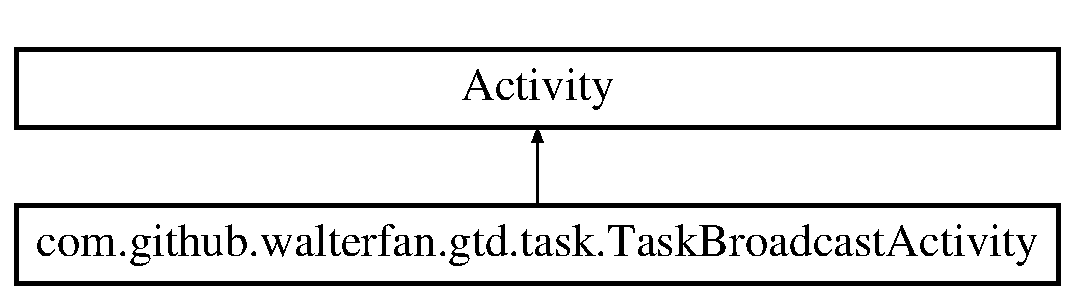
\includegraphics[height=2.000000cm]{classcom_1_1github_1_1walterfan_1_1gtd_1_1task_1_1TaskBroadcastActivity}
\end{center}
\end{figure}
\subsection*{Protected Member Functions}
\begin{DoxyCompactItemize}
\item 
\hypertarget{classcom_1_1github_1_1walterfan_1_1gtd_1_1task_1_1TaskBroadcastActivity_af1b8c2214d6c4fb6c2c371cb0a7a2453}{void {\bfseries on\-Create} (Bundle saved\-Instance\-State)}\label{classcom_1_1github_1_1walterfan_1_1gtd_1_1task_1_1TaskBroadcastActivity_af1b8c2214d6c4fb6c2c371cb0a7a2453}

\end{DoxyCompactItemize}


\subsection{Detailed Description}


Definition at line 13 of file Task\-Broadcast\-Activity.\-java.



The documentation for this class was generated from the following file\-:\begin{DoxyCompactItemize}
\item 
/cygdrive/d/workspace/java/\-G\-T\-D/src/com/github/walterfan/gtd/task/Task\-Broadcast\-Activity.\-java\end{DoxyCompactItemize}

\hypertarget{classcom_1_1github_1_1walterfan_1_1gtd_1_1task_1_1TaskBroadcastReceiver}{\section{com.\-github.\-walterfan.\-gtd.\-task.\-Task\-Broadcast\-Receiver Class Reference}
\label{classcom_1_1github_1_1walterfan_1_1gtd_1_1task_1_1TaskBroadcastReceiver}\index{com.\-github.\-walterfan.\-gtd.\-task.\-Task\-Broadcast\-Receiver@{com.\-github.\-walterfan.\-gtd.\-task.\-Task\-Broadcast\-Receiver}}
}
Inheritance diagram for com.\-github.\-walterfan.\-gtd.\-task.\-Task\-Broadcast\-Receiver\-:\begin{figure}[H]
\begin{center}
\leavevmode
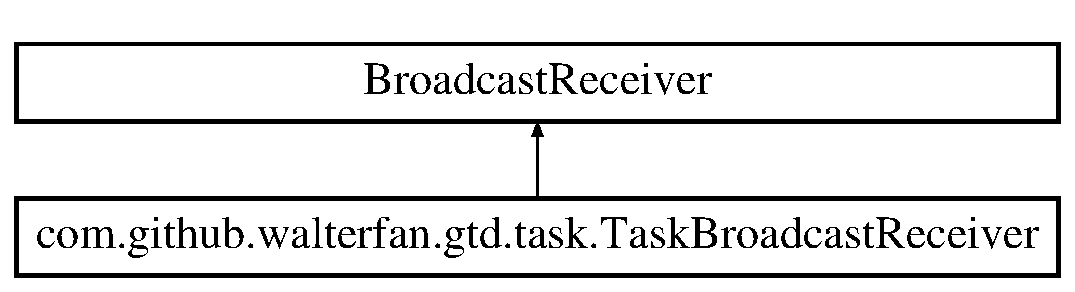
\includegraphics[height=2.000000cm]{classcom_1_1github_1_1walterfan_1_1gtd_1_1task_1_1TaskBroadcastReceiver}
\end{center}
\end{figure}
\subsection*{Public Member Functions}
\begin{DoxyCompactItemize}
\item 
\hypertarget{classcom_1_1github_1_1walterfan_1_1gtd_1_1task_1_1TaskBroadcastReceiver_a7e469a92165568aefe730aba4cab7bd4}{void {\bfseries on\-Receive} (Context context, Intent intent)}\label{classcom_1_1github_1_1walterfan_1_1gtd_1_1task_1_1TaskBroadcastReceiver_a7e469a92165568aefe730aba4cab7bd4}

\end{DoxyCompactItemize}


\subsection{Detailed Description}


Definition at line 7 of file Task\-Broadcast\-Receiver.\-java.



The documentation for this class was generated from the following file\-:\begin{DoxyCompactItemize}
\item 
/cygdrive/d/workspace/java/\-G\-T\-D/src/com/github/walterfan/gtd/task/Task\-Broadcast\-Receiver.\-java\end{DoxyCompactItemize}

\hypertarget{classcom_1_1github_1_1walterfan_1_1gtd_1_1ui_1_1TaskFragment}{\section{com.\-github.\-walterfan.\-gtd.\-ui.\-Task\-Fragment Class Reference}
\label{classcom_1_1github_1_1walterfan_1_1gtd_1_1ui_1_1TaskFragment}\index{com.\-github.\-walterfan.\-gtd.\-ui.\-Task\-Fragment@{com.\-github.\-walterfan.\-gtd.\-ui.\-Task\-Fragment}}
}
Inheritance diagram for com.\-github.\-walterfan.\-gtd.\-ui.\-Task\-Fragment\-:\begin{figure}[H]
\begin{center}
\leavevmode
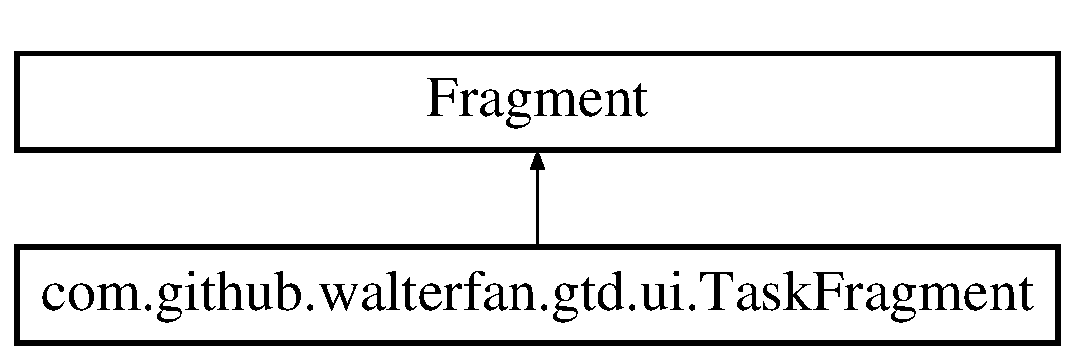
\includegraphics[height=2.000000cm]{classcom_1_1github_1_1walterfan_1_1gtd_1_1ui_1_1TaskFragment}
\end{center}
\end{figure}
\subsection*{Public Member Functions}
\begin{DoxyCompactItemize}
\item 
\hypertarget{classcom_1_1github_1_1walterfan_1_1gtd_1_1ui_1_1TaskFragment_ad9a7b86176e48b4d8b428725daa7cac6}{void {\bfseries on\-Create} (Bundle saved\-Instance\-State)}\label{classcom_1_1github_1_1walterfan_1_1gtd_1_1ui_1_1TaskFragment_ad9a7b86176e48b4d8b428725daa7cac6}

\item 
\hypertarget{classcom_1_1github_1_1walterfan_1_1gtd_1_1ui_1_1TaskFragment_a26c861ac1cde25cf11eddf621b4ebdae}{View {\bfseries on\-Create\-View} (Layout\-Inflater inflater, View\-Group container, Bundle saved\-Instance\-State)}\label{classcom_1_1github_1_1walterfan_1_1gtd_1_1ui_1_1TaskFragment_a26c861ac1cde25cf11eddf621b4ebdae}

\item 
\hypertarget{classcom_1_1github_1_1walterfan_1_1gtd_1_1ui_1_1TaskFragment_aca097f2af41861bdbd02ff23a76b0a84}{void {\bfseries on\-Pause} ()}\label{classcom_1_1github_1_1walterfan_1_1gtd_1_1ui_1_1TaskFragment_aca097f2af41861bdbd02ff23a76b0a84}

\item 
\hypertarget{classcom_1_1github_1_1walterfan_1_1gtd_1_1ui_1_1TaskFragment_a476771bb79bc3eb107934f1a4edbdc54}{void {\bfseries on\-Resume} ()}\label{classcom_1_1github_1_1walterfan_1_1gtd_1_1ui_1_1TaskFragment_a476771bb79bc3eb107934f1a4edbdc54}

\item 
\hypertarget{classcom_1_1github_1_1walterfan_1_1gtd_1_1ui_1_1TaskFragment_acc4ad151ef1e083bb1eaa4246e8da027}{void {\bfseries on\-Stop} ()}\label{classcom_1_1github_1_1walterfan_1_1gtd_1_1ui_1_1TaskFragment_acc4ad151ef1e083bb1eaa4246e8da027}

\end{DoxyCompactItemize}


\subsection{Detailed Description}


Definition at line 12 of file Task\-Fragment.\-java.



The documentation for this class was generated from the following file\-:\begin{DoxyCompactItemize}
\item 
/cygdrive/d/workspace/java/\-G\-T\-D/src/com/github/walterfan/gtd/ui/Task\-Fragment.\-java\end{DoxyCompactItemize}

\hypertarget{classcom_1_1github_1_1walterfan_1_1gtd_1_1ui_1_1TaskListViewAdapter}{\section{com.\-github.\-walterfan.\-gtd.\-ui.\-Task\-List\-View\-Adapter Class Reference}
\label{classcom_1_1github_1_1walterfan_1_1gtd_1_1ui_1_1TaskListViewAdapter}\index{com.\-github.\-walterfan.\-gtd.\-ui.\-Task\-List\-View\-Adapter@{com.\-github.\-walterfan.\-gtd.\-ui.\-Task\-List\-View\-Adapter}}
}
Inheritance diagram for com.\-github.\-walterfan.\-gtd.\-ui.\-Task\-List\-View\-Adapter\-:\begin{figure}[H]
\begin{center}
\leavevmode
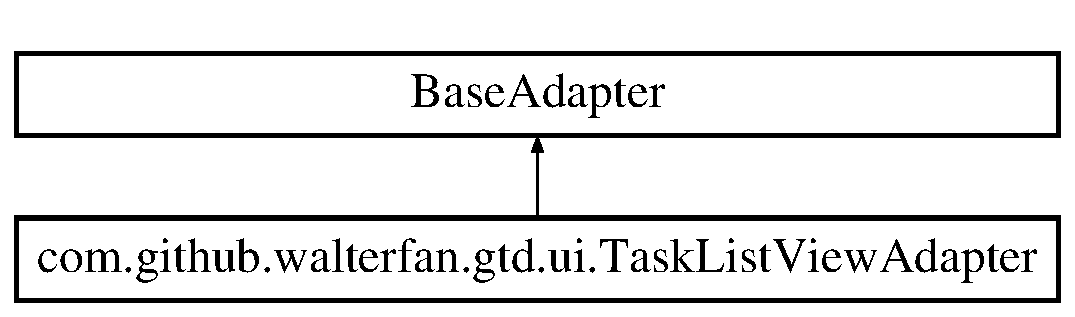
\includegraphics[height=2.000000cm]{classcom_1_1github_1_1walterfan_1_1gtd_1_1ui_1_1TaskListViewAdapter}
\end{center}
\end{figure}
\subsection*{Classes}
\begin{DoxyCompactItemize}
\item 
class {\bfseries View\-Holder}
\end{DoxyCompactItemize}
\subsection*{Public Member Functions}
\begin{DoxyCompactItemize}
\item 
\hypertarget{classcom_1_1github_1_1walterfan_1_1gtd_1_1ui_1_1TaskListViewAdapter_a16ce4f34c31ab4479a998b111e1d070b}{{\bfseries Task\-List\-View\-Adapter} (Context context, List$<$?extends Map$<$ String,?$>$$>$ data, int resource, String\mbox{[}$\,$\mbox{]} from, int\mbox{[}$\,$\mbox{]} to)}\label{classcom_1_1github_1_1walterfan_1_1gtd_1_1ui_1_1TaskListViewAdapter_a16ce4f34c31ab4479a998b111e1d070b}

\item 
\hypertarget{classcom_1_1github_1_1walterfan_1_1gtd_1_1ui_1_1TaskListViewAdapter_ae55097a4eba00793ba94dccdfb6924e5}{int {\bfseries get\-Count} ()}\label{classcom_1_1github_1_1walterfan_1_1gtd_1_1ui_1_1TaskListViewAdapter_ae55097a4eba00793ba94dccdfb6924e5}

\item 
\hypertarget{classcom_1_1github_1_1walterfan_1_1gtd_1_1ui_1_1TaskListViewAdapter_afa7348a72edd4f40b3aa3e240c4ebd23}{Object {\bfseries get\-Item} (int arg0)}\label{classcom_1_1github_1_1walterfan_1_1gtd_1_1ui_1_1TaskListViewAdapter_afa7348a72edd4f40b3aa3e240c4ebd23}

\item 
\hypertarget{classcom_1_1github_1_1walterfan_1_1gtd_1_1ui_1_1TaskListViewAdapter_a2289872d7e3292eaca44bc0fd00b8e78}{long {\bfseries get\-Item\-Id} (int arg0)}\label{classcom_1_1github_1_1walterfan_1_1gtd_1_1ui_1_1TaskListViewAdapter_a2289872d7e3292eaca44bc0fd00b8e78}

\item 
\hypertarget{classcom_1_1github_1_1walterfan_1_1gtd_1_1ui_1_1TaskListViewAdapter_ad3551650560e65d4b10baccb16af70ef}{View {\bfseries get\-View} (int position, View convert\-View, View\-Group parent)}\label{classcom_1_1github_1_1walterfan_1_1gtd_1_1ui_1_1TaskListViewAdapter_ad3551650560e65d4b10baccb16af70ef}

\end{DoxyCompactItemize}


\subsection{Detailed Description}


Definition at line 19 of file Task\-List\-View\-Adapter.\-java.



The documentation for this class was generated from the following file\-:\begin{DoxyCompactItemize}
\item 
/cygdrive/d/workspace/java/\-G\-T\-D/src/com/github/walterfan/gtd/ui/Task\-List\-View\-Adapter.\-java\end{DoxyCompactItemize}

\hypertarget{classcom_1_1github_1_1walterfan_1_1gtd_1_1ui_1_1TasksActivity}{\section{com.\-github.\-walterfan.\-gtd.\-ui.\-Tasks\-Activity Class Reference}
\label{classcom_1_1github_1_1walterfan_1_1gtd_1_1ui_1_1TasksActivity}\index{com.\-github.\-walterfan.\-gtd.\-ui.\-Tasks\-Activity@{com.\-github.\-walterfan.\-gtd.\-ui.\-Tasks\-Activity}}
}
Inheritance diagram for com.\-github.\-walterfan.\-gtd.\-ui.\-Tasks\-Activity\-:\begin{figure}[H]
\begin{center}
\leavevmode
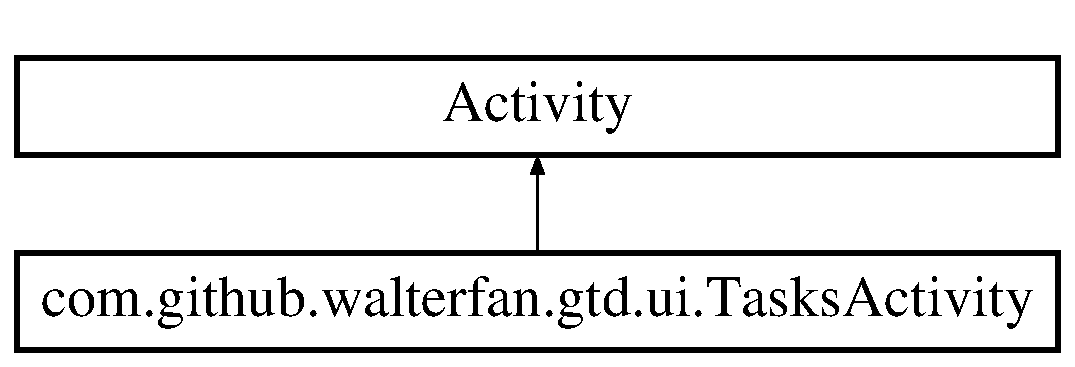
\includegraphics[height=2.000000cm]{classcom_1_1github_1_1walterfan_1_1gtd_1_1ui_1_1TasksActivity}
\end{center}
\end{figure}
\subsection*{Protected Member Functions}
\begin{DoxyCompactItemize}
\item 
\hypertarget{classcom_1_1github_1_1walterfan_1_1gtd_1_1ui_1_1TasksActivity_ab39743aa529abfc555671b7e5b9649ff}{void {\bfseries on\-Create} (Bundle saved\-Instance\-State)}\label{classcom_1_1github_1_1walterfan_1_1gtd_1_1ui_1_1TasksActivity_ab39743aa529abfc555671b7e5b9649ff}

\end{DoxyCompactItemize}


\subsection{Detailed Description}


Definition at line 18 of file Tasks\-Activity.\-java.



The documentation for this class was generated from the following file\-:\begin{DoxyCompactItemize}
\item 
/cygdrive/d/workspace/java/\-G\-T\-D/src/com/github/walterfan/gtd/ui/Tasks\-Activity.\-java\end{DoxyCompactItemize}

\hypertarget{classcom_1_1github_1_1walterfan_1_1gtd_1_1task_1_1TaskTimer}{\section{com.\-github.\-walterfan.\-gtd.\-task.\-Task\-Timer Class Reference}
\label{classcom_1_1github_1_1walterfan_1_1gtd_1_1task_1_1TaskTimer}\index{com.\-github.\-walterfan.\-gtd.\-task.\-Task\-Timer@{com.\-github.\-walterfan.\-gtd.\-task.\-Task\-Timer}}
}
\subsection*{Public Member Functions}
\begin{DoxyCompactItemize}
\item 
\hypertarget{classcom_1_1github_1_1walterfan_1_1gtd_1_1task_1_1TaskTimer_aaef721eae0f9573d9be02ca8a837b18c}{void {\bfseries start\-Count\-Down} ()}\label{classcom_1_1github_1_1walterfan_1_1gtd_1_1task_1_1TaskTimer_aaef721eae0f9573d9be02ca8a837b18c}

\item 
\hypertarget{classcom_1_1github_1_1walterfan_1_1gtd_1_1task_1_1TaskTimer_a624a14c9d1f28ac2cd058f36d2b0ccac}{void {\bfseries stop\-Count\-Down} ()}\label{classcom_1_1github_1_1walterfan_1_1gtd_1_1task_1_1TaskTimer_a624a14c9d1f28ac2cd058f36d2b0ccac}

\end{DoxyCompactItemize}


\subsection{Detailed Description}


Definition at line 8 of file Task\-Timer.\-java.



The documentation for this class was generated from the following file\-:\begin{DoxyCompactItemize}
\item 
/cygdrive/d/workspace/java/\-G\-T\-D/src/com/github/walterfan/gtd/task/Task\-Timer.\-java\end{DoxyCompactItemize}

\hypertarget{classcom_1_1github_1_1walterfan_1_1gtd_1_1task_1_1TaskViewManager}{\section{com.\-github.\-walterfan.\-gtd.\-task.\-Task\-View\-Manager Class Reference}
\label{classcom_1_1github_1_1walterfan_1_1gtd_1_1task_1_1TaskViewManager}\index{com.\-github.\-walterfan.\-gtd.\-task.\-Task\-View\-Manager@{com.\-github.\-walterfan.\-gtd.\-task.\-Task\-View\-Manager}}
}
\subsection*{Public Member Functions}
\begin{DoxyCompactItemize}
\item 
\hypertarget{classcom_1_1github_1_1walterfan_1_1gtd_1_1task_1_1TaskViewManager_a817ebc057b16d9aad7772ad6081bc303}{String {\bfseries get\-From\-Asset} (Activity activity, String file\-Name)}\label{classcom_1_1github_1_1walterfan_1_1gtd_1_1task_1_1TaskViewManager_a817ebc057b16d9aad7772ad6081bc303}

\item 
\hypertarget{classcom_1_1github_1_1walterfan_1_1gtd_1_1task_1_1TaskViewManager_adb4e7a3473a2ca7d5f160570acc96617}{void {\bfseries list\-Tasks} ()}\label{classcom_1_1github_1_1walterfan_1_1gtd_1_1task_1_1TaskViewManager_adb4e7a3473a2ca7d5f160570acc96617}

\end{DoxyCompactItemize}


\subsection{Detailed Description}


Definition at line 9 of file Task\-View\-Manager.\-java.



The documentation for this class was generated from the following file\-:\begin{DoxyCompactItemize}
\item 
/cygdrive/d/workspace/java/\-G\-T\-D/src/com/github/walterfan/gtd/task/Task\-View\-Manager.\-java\end{DoxyCompactItemize}

\hypertarget{classcom_1_1github_1_1walterfan_1_1gtd_1_1test_1_1TestActivity}{\section{com.\-github.\-walterfan.\-gtd.\-test.\-Test\-Activity Class Reference}
\label{classcom_1_1github_1_1walterfan_1_1gtd_1_1test_1_1TestActivity}\index{com.\-github.\-walterfan.\-gtd.\-test.\-Test\-Activity@{com.\-github.\-walterfan.\-gtd.\-test.\-Test\-Activity}}
}
Inheritance diagram for com.\-github.\-walterfan.\-gtd.\-test.\-Test\-Activity\-:\begin{figure}[H]
\begin{center}
\leavevmode
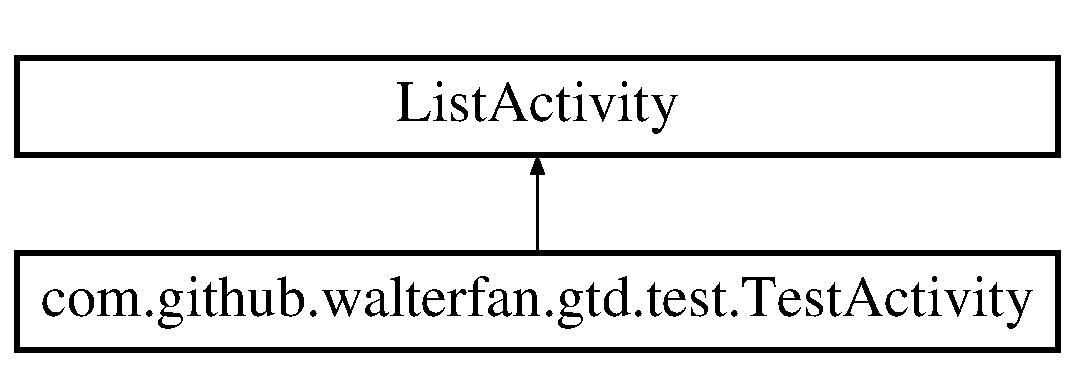
\includegraphics[height=2.000000cm]{classcom_1_1github_1_1walterfan_1_1gtd_1_1test_1_1TestActivity}
\end{center}
\end{figure}
\subsection*{Protected Member Functions}
\begin{DoxyCompactItemize}
\item 
\hypertarget{classcom_1_1github_1_1walterfan_1_1gtd_1_1test_1_1TestActivity_a9ae50fcdb8df9d0e5381593a52b46e9a}{void {\bfseries on\-Create} (Bundle saved\-Instance\-State)}\label{classcom_1_1github_1_1walterfan_1_1gtd_1_1test_1_1TestActivity_a9ae50fcdb8df9d0e5381593a52b46e9a}

\item 
\hypertarget{classcom_1_1github_1_1walterfan_1_1gtd_1_1test_1_1TestActivity_a12c48a0db11e934eb1452888ad3cb2df}{void {\bfseries on\-List\-Item\-Click} (List\-View l, View v, int position, long id)}\label{classcom_1_1github_1_1walterfan_1_1gtd_1_1test_1_1TestActivity_a12c48a0db11e934eb1452888ad3cb2df}

\end{DoxyCompactItemize}


\subsection{Detailed Description}


Definition at line 14 of file Test\-Activity.\-java.



The documentation for this class was generated from the following file\-:\begin{DoxyCompactItemize}
\item 
/cygdrive/d/workspace/java/\-G\-T\-D/src/com/github/walterfan/gtd/test/Test\-Activity.\-java\end{DoxyCompactItemize}

\hypertarget{classcom_1_1github_1_1walterfan_1_1gtd_1_1parcel_1_1User}{\section{com.\-github.\-walterfan.\-gtd.\-parcel.\-User Class Reference}
\label{classcom_1_1github_1_1walterfan_1_1gtd_1_1parcel_1_1User}\index{com.\-github.\-walterfan.\-gtd.\-parcel.\-User@{com.\-github.\-walterfan.\-gtd.\-parcel.\-User}}
}
Inheritance diagram for com.\-github.\-walterfan.\-gtd.\-parcel.\-User\-:\begin{figure}[H]
\begin{center}
\leavevmode
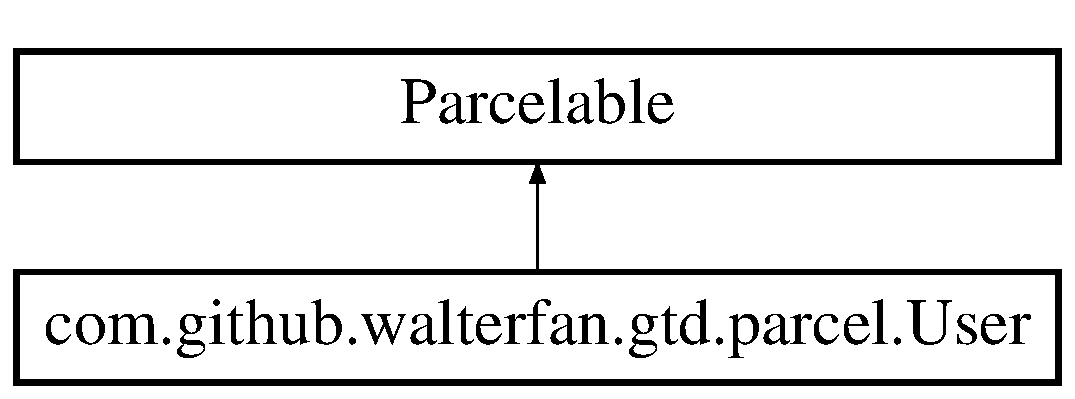
\includegraphics[height=2.000000cm]{classcom_1_1github_1_1walterfan_1_1gtd_1_1parcel_1_1User}
\end{center}
\end{figure}
\subsection*{Public Member Functions}
\begin{DoxyCompactItemize}
\item 
\hypertarget{classcom_1_1github_1_1walterfan_1_1gtd_1_1parcel_1_1User_a022a6d9b44e2bbddef063e959c5640fc}{int {\bfseries describe\-Contents} ()}\label{classcom_1_1github_1_1walterfan_1_1gtd_1_1parcel_1_1User_a022a6d9b44e2bbddef063e959c5640fc}

\item 
\hypertarget{classcom_1_1github_1_1walterfan_1_1gtd_1_1parcel_1_1User_aebc736bb2e6396cd49f94ed49e3f31d3}{void {\bfseries write\-To\-Parcel} (Parcel dest, int flags)}\label{classcom_1_1github_1_1walterfan_1_1gtd_1_1parcel_1_1User_aebc736bb2e6396cd49f94ed49e3f31d3}

\item 
\hypertarget{classcom_1_1github_1_1walterfan_1_1gtd_1_1parcel_1_1User_acdf229bb23ca6a0e747fc57a7a1b0551}{String {\bfseries get\-User\-Name} ()}\label{classcom_1_1github_1_1walterfan_1_1gtd_1_1parcel_1_1User_acdf229bb23ca6a0e747fc57a7a1b0551}

\item 
\hypertarget{classcom_1_1github_1_1walterfan_1_1gtd_1_1parcel_1_1User_af8a7dcbb792911d639d96a486310bd35}{void {\bfseries set\-User\-Name} (String user\-Name)}\label{classcom_1_1github_1_1walterfan_1_1gtd_1_1parcel_1_1User_af8a7dcbb792911d639d96a486310bd35}

\item 
\hypertarget{classcom_1_1github_1_1walterfan_1_1gtd_1_1parcel_1_1User_aded61ba54a3ab71b6b57606cf88546f6}{String {\bfseries get\-Password} ()}\label{classcom_1_1github_1_1walterfan_1_1gtd_1_1parcel_1_1User_aded61ba54a3ab71b6b57606cf88546f6}

\item 
\hypertarget{classcom_1_1github_1_1walterfan_1_1gtd_1_1parcel_1_1User_a49c6f07f2523d19b00159ad508e97947}{void {\bfseries set\-Password} (String password)}\label{classcom_1_1github_1_1walterfan_1_1gtd_1_1parcel_1_1User_a49c6f07f2523d19b00159ad508e97947}

\end{DoxyCompactItemize}
\subsection*{Static Public Attributes}
\begin{DoxyCompactItemize}
\item 
static final \\*
Parcelable.\-Creator$<$ \hyperlink{classcom_1_1github_1_1walterfan_1_1gtd_1_1parcel_1_1User}{User} $>$ {\bfseries C\-R\-E\-A\-T\-O\-R}
\end{DoxyCompactItemize}


\subsection{Detailed Description}


Definition at line 6 of file User.\-java.



\subsection{Member Data Documentation}
\hypertarget{classcom_1_1github_1_1walterfan_1_1gtd_1_1parcel_1_1User_a42f8199f5f8617c4026624a50ac743cc}{\index{com\-::github\-::walterfan\-::gtd\-::parcel\-::\-User@{com\-::github\-::walterfan\-::gtd\-::parcel\-::\-User}!C\-R\-E\-A\-T\-O\-R@{C\-R\-E\-A\-T\-O\-R}}
\index{C\-R\-E\-A\-T\-O\-R@{C\-R\-E\-A\-T\-O\-R}!com::github::walterfan::gtd::parcel::User@{com\-::github\-::walterfan\-::gtd\-::parcel\-::\-User}}
\subsubsection[{C\-R\-E\-A\-T\-O\-R}]{\setlength{\rightskip}{0pt plus 5cm}final Parcelable.\-Creator$<${\bf User}$>$ com.\-github.\-walterfan.\-gtd.\-parcel.\-User.\-C\-R\-E\-A\-T\-O\-R\hspace{0.3cm}{\ttfamily [static]}}}\label{classcom_1_1github_1_1walterfan_1_1gtd_1_1parcel_1_1User_a42f8199f5f8617c4026624a50ac743cc}
{\bfseries Initial value\-:}
\begin{DoxyCode}
= \textcolor{keyword}{new} Creator<User> () \{
        @Override
        \textcolor{keyword}{public} User createFromParcel(Parcel source) \{
            User user = \textcolor{keyword}{new} User();
            user.userName = source.readString();
            user.password = source.readString();
            \textcolor{keywordflow}{return} user;
        \}
        
        @Override
        \textcolor{keyword}{public} User[] newArray(\textcolor{keywordtype}{int} size) \{
            \textcolor{keywordflow}{return} \textcolor{keyword}{new} User[size];
        \}
    \}
\end{DoxyCode}


Definition at line 10 of file User.\-java.



The documentation for this class was generated from the following file\-:\begin{DoxyCompactItemize}
\item 
/cygdrive/d/workspace/java/\-G\-T\-D/src/com/github/walterfan/gtd/parcel/User.\-java\end{DoxyCompactItemize}

\hypertarget{classcom_1_1github_1_1walterfan_1_1gtd_1_1service_1_1UserService}{\section{com.\-github.\-walterfan.\-gtd.\-service.\-User\-Service Class Reference}
\label{classcom_1_1github_1_1walterfan_1_1gtd_1_1service_1_1UserService}\index{com.\-github.\-walterfan.\-gtd.\-service.\-User\-Service@{com.\-github.\-walterfan.\-gtd.\-service.\-User\-Service}}
}
Inheritance diagram for com.\-github.\-walterfan.\-gtd.\-service.\-User\-Service\-:\begin{figure}[H]
\begin{center}
\leavevmode
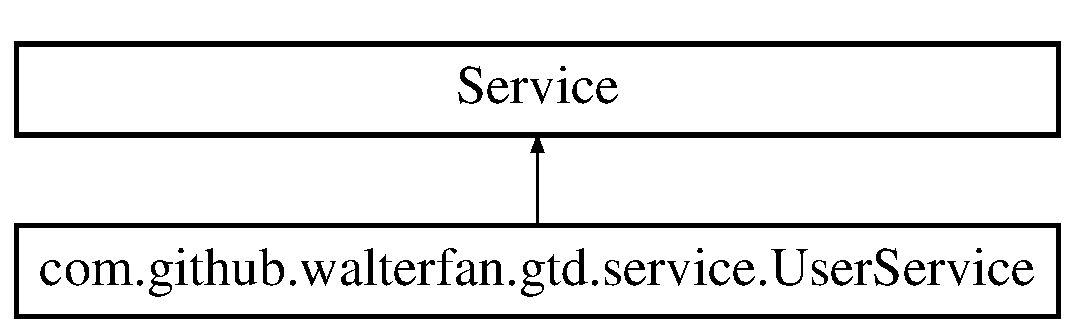
\includegraphics[height=2.000000cm]{classcom_1_1github_1_1walterfan_1_1gtd_1_1service_1_1UserService}
\end{center}
\end{figure}
\subsection*{Public Member Functions}
\begin{DoxyCompactItemize}
\item 
\hypertarget{classcom_1_1github_1_1walterfan_1_1gtd_1_1service_1_1UserService_a4d5b299bdc1ef04107330016f65954af}{I\-Binder {\bfseries on\-Bind} (Intent intent)}\label{classcom_1_1github_1_1walterfan_1_1gtd_1_1service_1_1UserService_a4d5b299bdc1ef04107330016f65954af}

\end{DoxyCompactItemize}


\subsection{Detailed Description}


Definition at line 7 of file User\-Service.\-java.



The documentation for this class was generated from the following file\-:\begin{DoxyCompactItemize}
\item 
/cygdrive/d/workspace/java/\-G\-T\-D/src/com/github/walterfan/gtd/service/User\-Service.\-java\end{DoxyCompactItemize}

%--- End generated contents ---

% Index
\newpage
\phantomsection
\addcontentsline{toc}{chapter}{Index}
\printindex

\end{document}
